\section{Evaluation}
\label{sec:evaluation}

To evaluate the performance of our proposed techniques, we conduct large-scale simulations over
two settings based on two different propagation models. In particular, we consider the log-distance-based
propagation model and the Longley--Rice model obtained from SPLAT!~\cite{splat}. We evaluate various 
algorithms, using multiple performance metrics as described below. 

\para{Performance Metrics.} We use the following metrics 1, 2, and 3 to evaluate the localization methods and use the 4th metric to evaluate the power estimation methods.
\begin{enumerate}
    \item Localization Error ($\lerr$)
    \item Miss rate ($\mr$)
    \item False Alarm rate ($\fr$)
    \item Power Error ($\perr$)
\end{enumerate}
Given a multi-transmitter localization solution, we first compute the $\lerr$ as
the minimum-cost matching in the bi-partite graph over the
ground truth and the solution's locations, where the cost of each edge in the graph is the Euclidean distance between the matched ground truth node location and the solution's node location.
We use a simple greedy algorithm to compute the min-cost matching.
%%%%
The unmatched nodes are regarded as false alarms or misses. 
We also put an upper threshold on the cost ($\lerr$) of an eligible match. 
E.g., if there are four intruders in reality, but the algorithm predicts six
intruders then it is said to incur zero misses and two false alarms, so the $\mr$ is zero and the $\fr$ is one-third. 
If the algorithm predicts three intruders then it incurs one miss and zero false alarms, so the $\mr$ is one-fourth and the $\fr$ is zero.
In the plots, we stack the miss rate and false alarm rate to reflect the overall performance.


\para{Algorithms Compared.} 
We implement\footnote{Source code at: \url{https://github.com/caitaozhan/deeplearning-localization}.} and compare six algorithms in two stages. In stage one, we compare three versions of our
techniques, viz., \our, \ouryolo, and \ourpeak.  Recall that \our, \ouryolo, and \ourpeak 
use \imgimg in the first step, and \yolocust, original YOLOv3, and \simpeak respectively in the second step. In the first stage of our evaluations, we will show that 
\our outperforms \ouryolo and \ourpeak in almost all performance metrics. 
Thus, in the second stage, we only compare \our with
schemes from three prior works, viz., \splot~\cite{mobicom17-splot}, \deeptx~\cite{icccn20-deeptxfinder},
and \map~\cite{ipsn20-mtl} and show that \our outperforms the prior works.

\para{Training and Testing Dataset.}
We consider an area
%\footnote{To deal with areas of larger than 1 square kilometers, a tiling method similar to the one in \cite{icccn20-deeptxfinder} can be used. Tiling is not the focus of this work.} 
of $1km \times 1km$, and use grid cells (pixels) of 
$10 m \times 10 m$, so the grid is $100\times100$. 
The transmitters may be deployed
anywhere within a cell (i.e., their location is in the continuous
domain), while the sensors are deployed at the centers of the grid cells (i.e. their location is in the discrete domain).
%%%%%%%
For each instance (training or test sample), the said number of sensors and transmitters are deployed in the field randomly. 
For each of the two settings (propagation models described below), we create a 100,000 sample training dataset to train our models and create another 20,000 sample testing dataset to evaluate the trained model. 
%\red{Each dataset consists of samples with varying  number of transmitter, 
%varying sensor density, and varying transmitter power (0 to 5 dBm). 
%Even for the same sensor density, training  and testing samples may have sensors
%at different locations.}

We will evaluate the performance of various techniques for
varying number of transmitters/intruders and sensor
density. When we vary a specific parameter, the other parameter
is set to its \emph{default} value; the number of transmitters varies from 1 to 10 and the default value is 5; the sensor density varies from 1\% to 10\% and the default value is 6\% (600  sensors in a $100\times100$ grid).
The two default numbers 5 and 6\% are chosen because they are in the middle of their ranges.
When not mentioned, the default values are used.
The transmitter power varies from 0 to 5 dBm and is randomly picked.
To minimize overfitting, the training dataset and testing dataset have sensors placed at completely different locations.
%%%%%%%%%%%%%%%%%%%%%%%%%%%%%%%%%%%

We train the \our model using the 100,000 sample dataset. To train the \deeptx~\cite{icccn20-deeptxfinder}, we partition the 100,000 sample training dataset into ten datasets based on the number of transmitters in the samples which varies from 1 to 10. 
These ten datasets are used to train the ten ``localization" CNN models in \deeptx, and the full dataset of 100,000 samples is used to train the \deeptx model that determines the number of transmitters. 
%%%%%%%%%
For the \map scheme~\cite{ipsn20-mtl}, we assume the availability of all required probability distributions. We note that using a simple cost model (number of samples need to be gathered), 
the overall training cost for \map is an order of magnitude higher than \our and \deeptx. 
Lastly, \splot~\cite{mobicom17-splot} does not require any training.




%%%%%%%%%%%%%%

\para{Two Propagation Models and Settings}.
The sensor readings (i.e. the dataset) are simulated based on a propagation model~\cite{yuning2023}. 
% Note that the propagation model is only used to simulate/generate samples, and the techniques developed themselves do not assume any propagation model. 
To demonstrate the generality of our techniques, we consider two propagation models as described below. 

\softpara{Log-Distance Propagation Model and Setting.}
Log-Distance propagation model is a generic model that extends Friis Free space model 
which is used to predict the path loss for a wide range of environments. 
As per this model, the path loss (in dB) between 
two points $x$ and $y$ at a distance $d$ is given by: $PL_d = 10\alpha\log{d} + \mathcal{X},$
where $\alpha$ (we use 3.5) is the path-loss exponent and $\mathcal{X}$ represents the shadowing effect that can be represented by a zero-mean Gaussian distribution with a certain (we use 1) standard deviation. 
Power received (in dBm) at point $y$ due to a transmitter at point $x$ with a 
transmit power of $P_x$ is thus: $P_{x} - PL_d$.
Power received at point $y$ due to multiple sources is assumed to be just an 
aggregate  of the powers (in linear) received from each of the sources.

% In this subsection, we evaluate our techniques on a data set generated from a more realistic propagation model, the Longley-Rice ~\cite{chamberlin82} Irregular Terrain With Obstruction Model (ITWOM). 
% We conduct one set of experiments based on this data set. We compare \our with \deeptx, \map, and \splot, and show \our is better.

\softpara{SPLAT! Model and Setting.}
This is a complex model of wireless propagation based on many parameters including locations, terrain data, obstructions, soil conditions, etc.
We use \splat~\cite{splat} to generate path-loss values. \splat is an open-source software implementing the Longley-Rice ~\cite{chamberlin82} Irregular Terrain With Obstruction Model (ITWOM) model.
%%%%%%%%%%%%%%%%%%%%
We consider a random area in Long Island, New York of $1km \times 1km$ large and use the 600 MHz band to generate path losses.
% As the height of an entity is an important factor in determining the
% path loss, we place the transmitters (PU or SU) at a height of 30m and the 
% receivers (PURs and SSs) at 15m above the ground level.


%%%%%%%% compare ours $$$$$$$$$$$$$

\begin{figure}[ht]
	\centering
	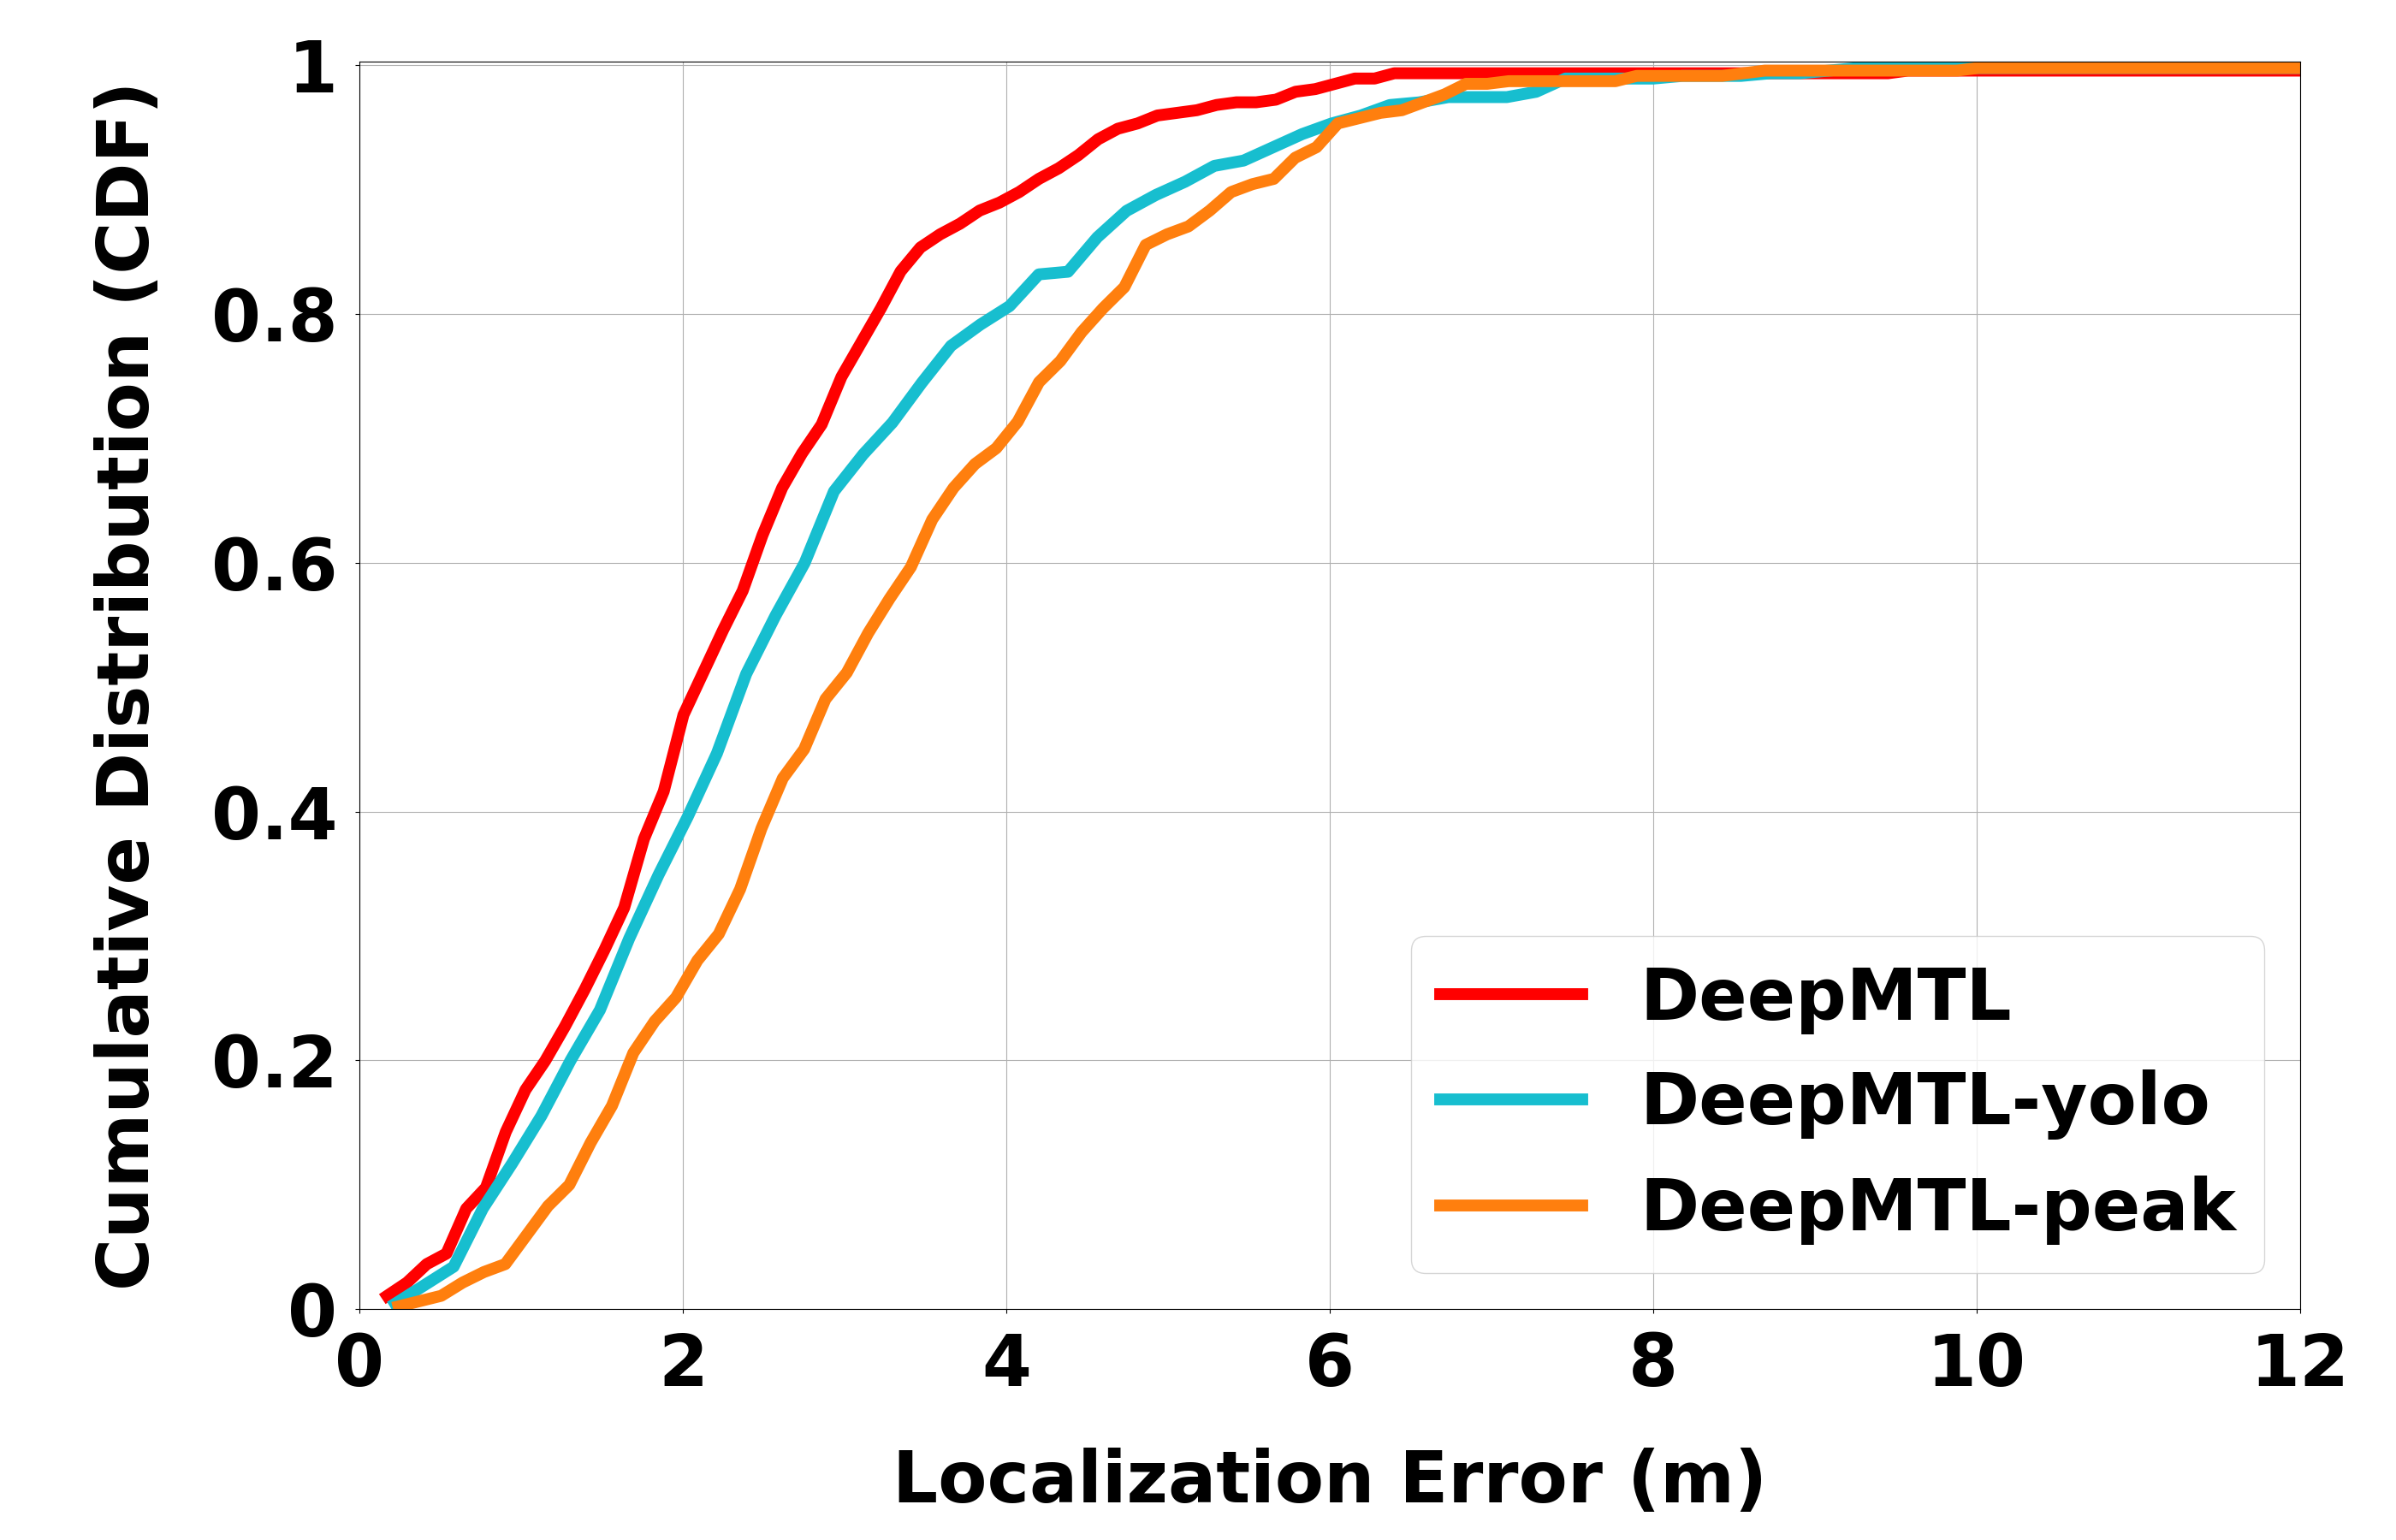
\includegraphics[width=0.6\textwidth]{chapters/wowmom-pmc/figures/ours_cdf.png}
	\caption{Cumulative probability of localization error of \our, \ouryolo and \ourpeak, for the special case of single transmitter localization with 6\% sensor density.}
	\label{fig:ours_cdf}
\end{figure}

\begin{figure}[ht]
	\centering
	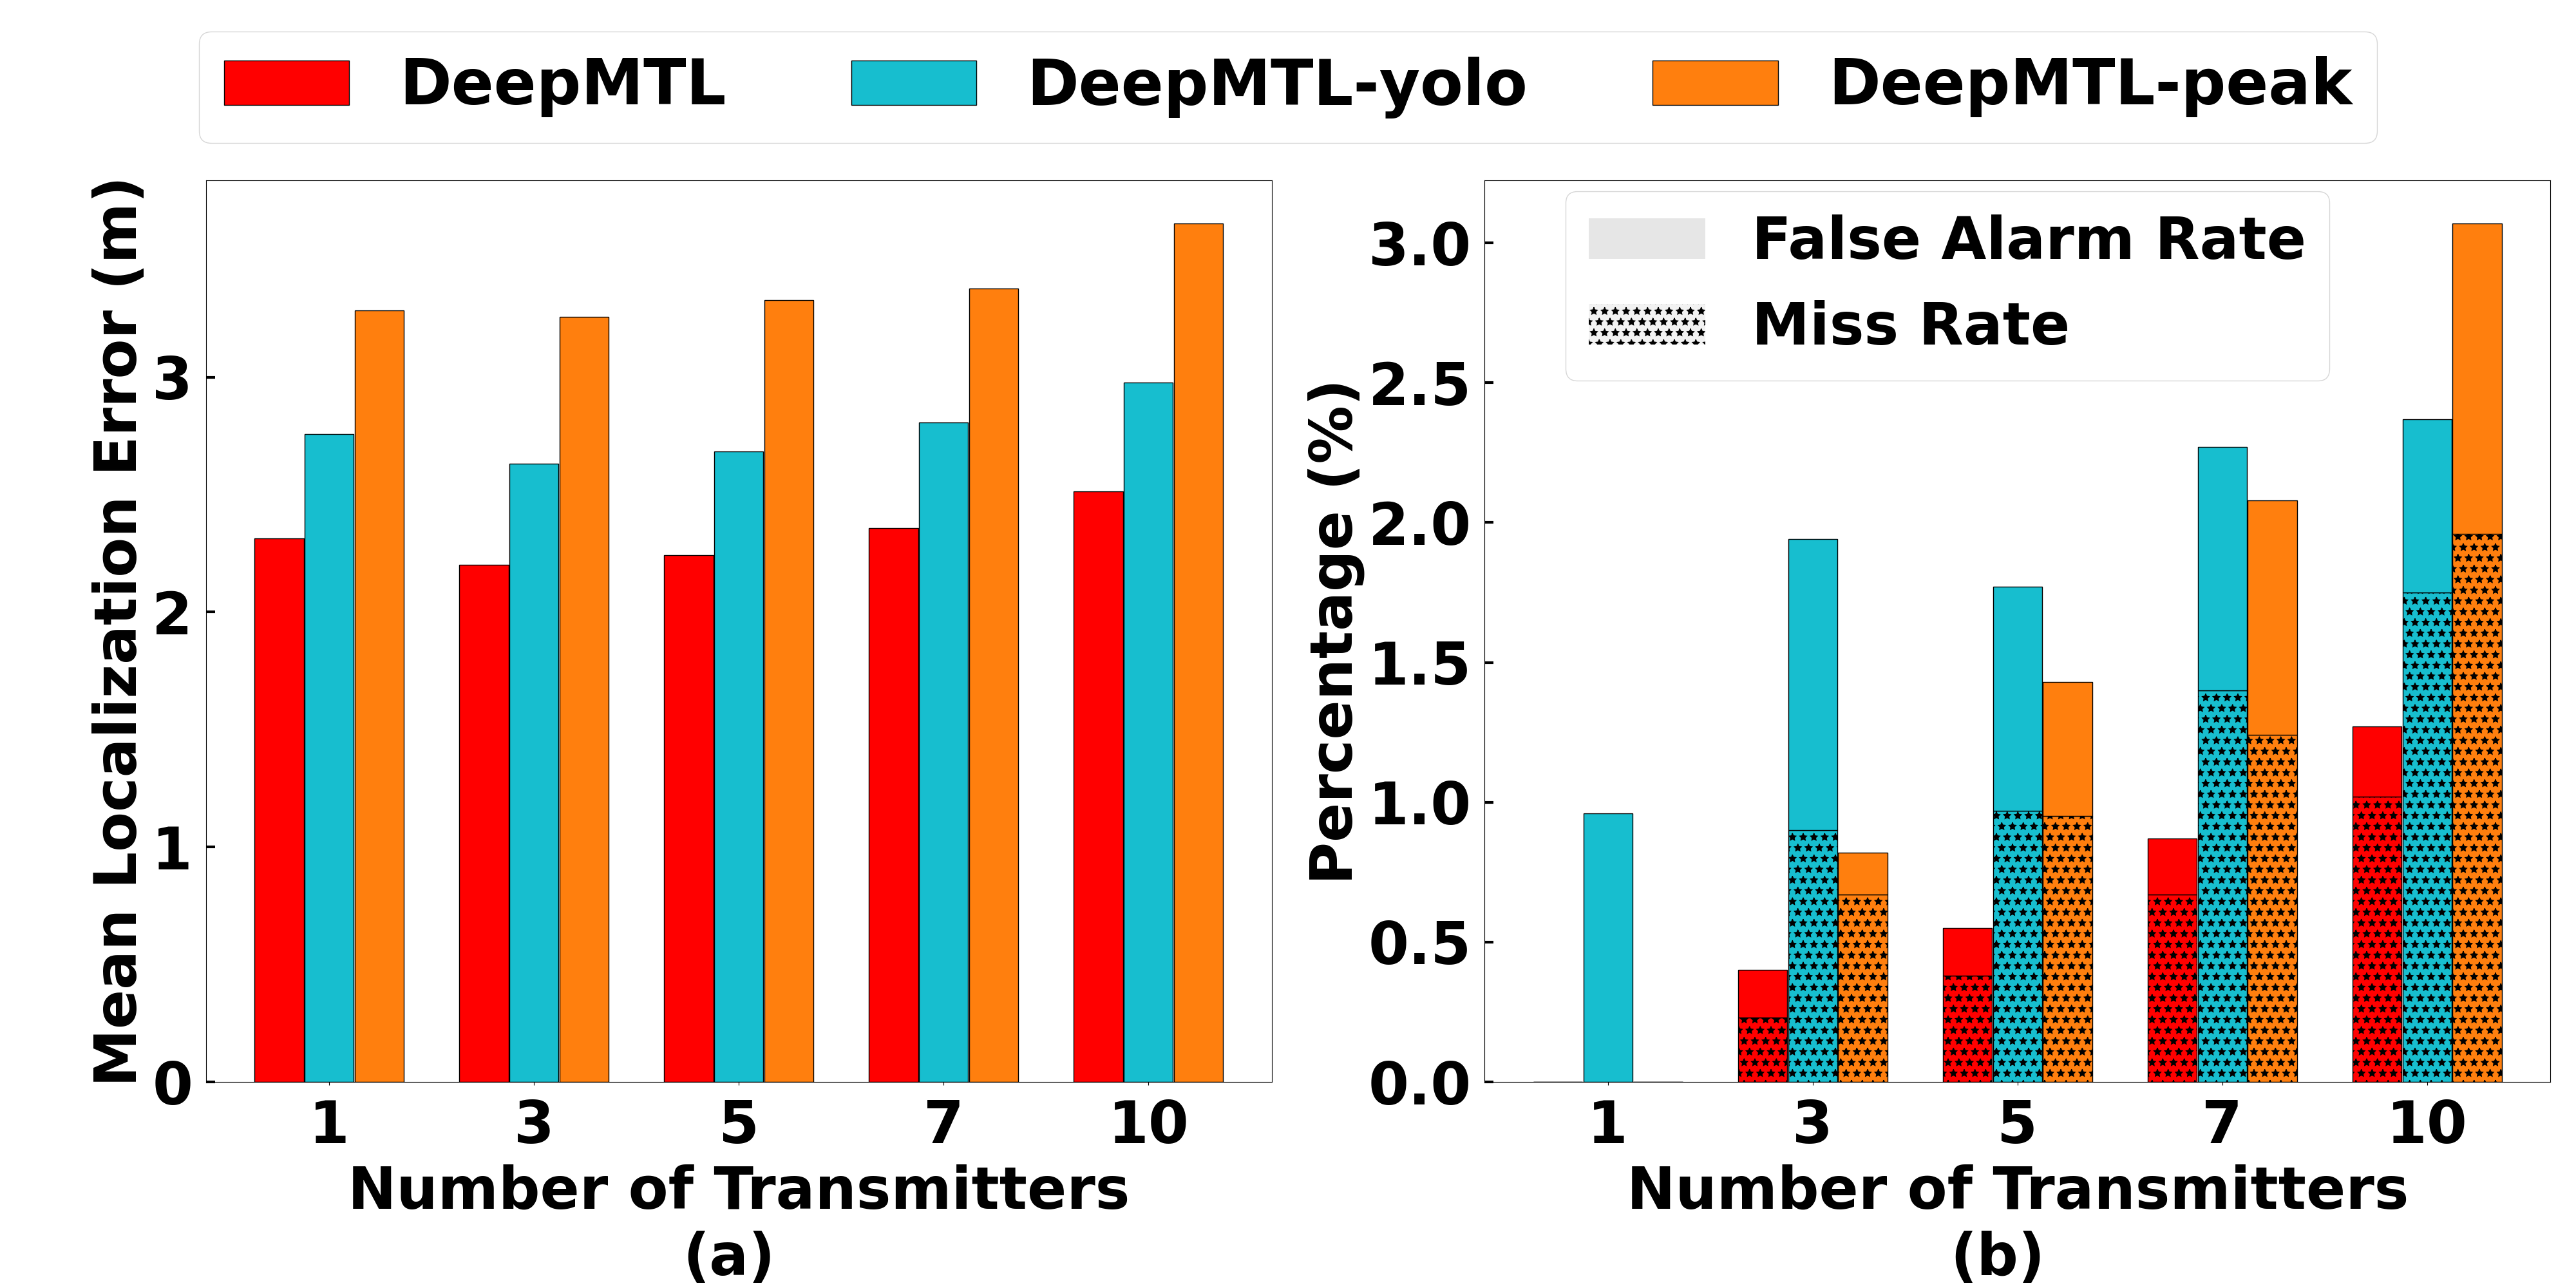
\includegraphics[width=0.75\textwidth]{chapters/wowmom-pmc/figures/ours_error_missfalse_vary_numintru.png}
	\caption{(a) Localization error and (b) miss and false alarm rates, of \our, \ouryolo and \ourpeak variants for varying number of transmitters in log-distance dataset (propagation) model.}
	\label{fig:ours_vary_numintru}
\end{figure}

\begin{figure}[ht]
	\centering
	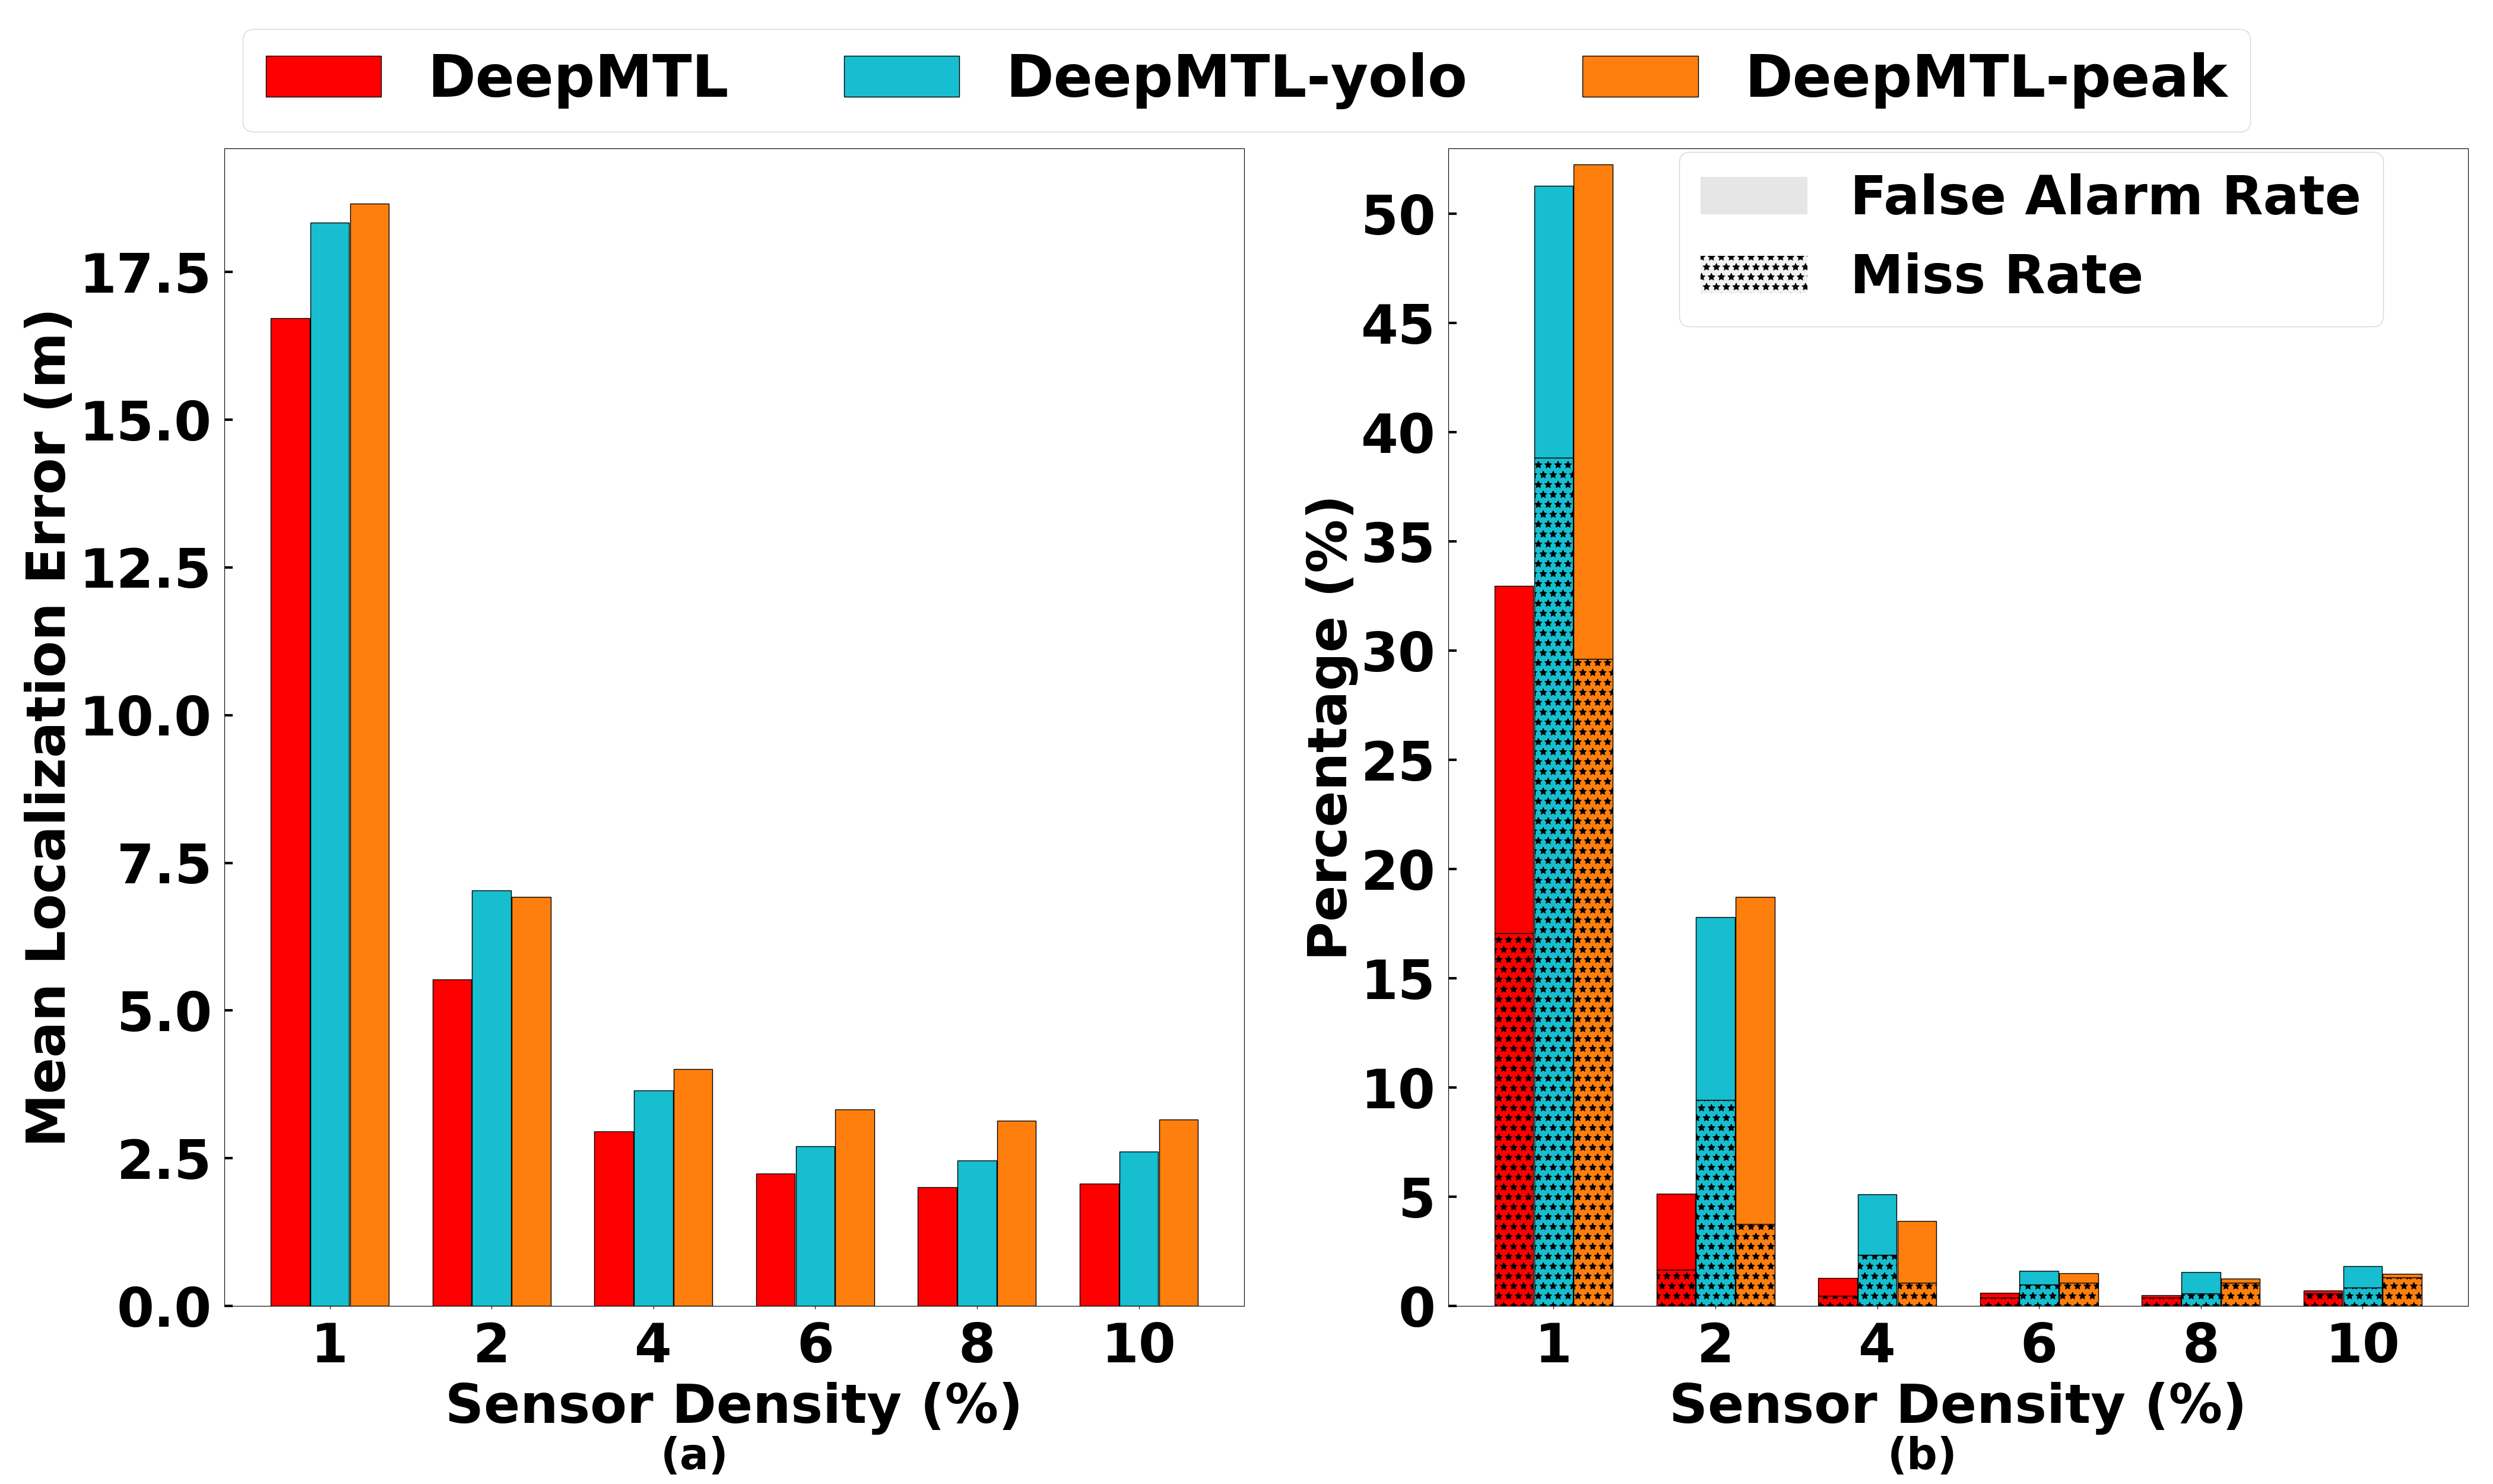
\includegraphics[width=0.75\textwidth]{chapters/wowmom-pmc/figures/ours_error_missfalse_vary_sendensity.png}
	\caption{(a) Localization error and (b) miss and false alarm rates, of \our, \ouryolo and \ourpeak variants for varying sensor density in log-distance dataset (propagation) model.}
	\label{fig:ours_vary_sendensity}
\end{figure}



\subsection{\our vs.\ \ouryolo vs.\ \ourpeak}

In this subsection, we compare the three variants of our technique, viz., \our, \ouryolo, and
\ourpeak. For simplicity, we only show plots for the log-distance propagation model setting in this 
subsection (we observed similar performance trends for the Longley-Rice propagation model too). 
%%%%%%%%%%%%%%%%%%%%%%%%%%%%%

\softpara{Performance Results.}
In Fig.~\ref{fig:ours_cdf}, we plot  the cumulative density function (CDF) of the localization
error, for the simple case of a single transmitter.
We observe that \our outperforms the other variants, as it yields a higher cumulative probability for a lower range of errors.
%%%%%%%%%%%%%%%%%%%
In addition, we evaluate the three variants for varying number of transmitters (Fig.~\ref{fig:ours_vary_numintru}) and sensor density (Fig.~\ref{fig:ours_vary_sendensity}), and evaluate the localization error as well as the false alarm and miss rates. 
%%%%%%%%%%%%%%%%
We observe that \our consistently outperforms the other two variants 
across all plots and performance metrics. As expected, the performance of all algorithms 
degrades with an increase in the number of transmitters (in terms of false alarms and miss rates) or with a decrease in sensor density. 
In general, the localization error of \our is around 15-30\% lower than the other variants.
Impressively, the total cardinality error (i.e., false alarms plus miss rates) is fewer than 1\% for the \our technique, when the sensor density is 6\% or above.

When the sensor density is as low as 1\%, the performance of all methods significantly decreases.
Because when the sensor density is 1\% or lower, the input image will be very sparse and contain only a few pixels.
\our's first part \imgimg has a receptive field of $17\times17$.
This area will contain an average of less than three sensors when the sensor density is 1\% ($17\times17\times0.01=2.89$).
This number is considered too low and note that 2.89 sensors are not enough for the trilateration localization method, which needs three sensors.
Our CNN models need to function well with enough pixels that contain useful information. 
So we suggest the sensor density to be at least 2\% to achieve reasonable results.

\begin{table}[ht]
	\centering
	\caption{Compare Localization Running Time (s) for 1 to 10 Number of Intruders}
	\vspace{-0.1in}
	\begin{tabular}{c c c c c c c}
		\hline\hline
		\small{Intru.} & \small{\ourpeak}  & \small{\ouryolo} & \small{\our} & \small{\map} & \small{\splot} & \small{\deeptx} \\
		\hline
		1 & 0.0013 & 0.0180 & 0.0180 & 8.78 & 1.53 & 0.0015 \\ 
		3 & 0.0014 & 0.0183 &  0.0186 & 15.1 & 1.79 & 0.0016 \\
		5 & 0.0016 & 0.0192 &  0.0189 & 19.3 & 2.06 & 0.0017\\
		7 & 0.0018 & 0.0196 &  0.0194 & 24.1 & 2.32 & 0.0019 \\
		10 & 0.0023 & 0.0205 & 0.0206 & 28.5 & 2.72 & 0.0022 \\
		\hline
	\end{tabular}
	\label{table:running-time}	
\end{table}


\softpara{Running Time Comparison.} For the running time comparison of the variants, see Table \ref{table:running-time}. 
Our hardware is an Intel i7-8700 CPU and an Nvidia RTX 2070 GPU. 
We observe that, as expected, \our and \ouryolo which use a sophisticated object-detection method do incur higher latency (around 20 milliseconds) than \ourpeak (around two milliseconds). As our key
performance criteria is accuracy and the run time of \our is still quite low, we choose \our for comparison with the prior works in ~\S\ref{subsec:vs_prior}. 


\softpara{Localizing Transmitters Close By.}
Localizing two or more transmitters close by is a hard part of the \mtl problem.
Fig.~\ref{fig:peaks}(c) and (d) gives an example of when an advanced object detection algorithm will work while a simple local maximal peak detection might not.
Fig.~\ref{fig:peaks}(c) and (d) shows \our can successfully localize two transmitters as close as three pixels apart.
When a pixel represents a $10m \times 10m$ area, then it is 30 meters apart.
If a pixel represents a smaller area, such as $1m \times 1m$, it has the potential to localize two transmitters as close as three meters apart.

\softpara{Two YOLO Thresholds.} YOLO has two important thresholds to tune that can affect the miss rate and false alarm rate. 
One is the confidence threshold (\conf) and the other is the non-maximum suppression threshold (\nms).
An object will be recognized as a peak only if its confidence level is larger than \conf.
If two recognized peaks' bounding boxes have a large overlap, and their intersection of union is higher than \nms, then the two peaks will be considered as one peak. 
The peak with a higher confidence level keeps while the other peak with a lower confidence level discards.
A higher \conf will bring a lower false alarm rate but a higher miss rate, and a higher \nms will bring a lower miss rate but a higher false alarm rate.
We pick \conf= 0.8 and \nms= 0.5 for \our as we observe these values bring a good balance between false alarm rate and miss rate.
In particular, a high \conf of 0.8  precludes ``fake peaks" at locations with no transmitters.
Also, a low \nms weakens \our's ability to localize two close by transmitters, while a high $nms$ yields
a high false alarm rate (by incorrectly interpreting a single transmitter as multiple close by transmitters); thus, we chose \nms of 0.5.


% \begin{figure}[h]
% 	\centering
% 	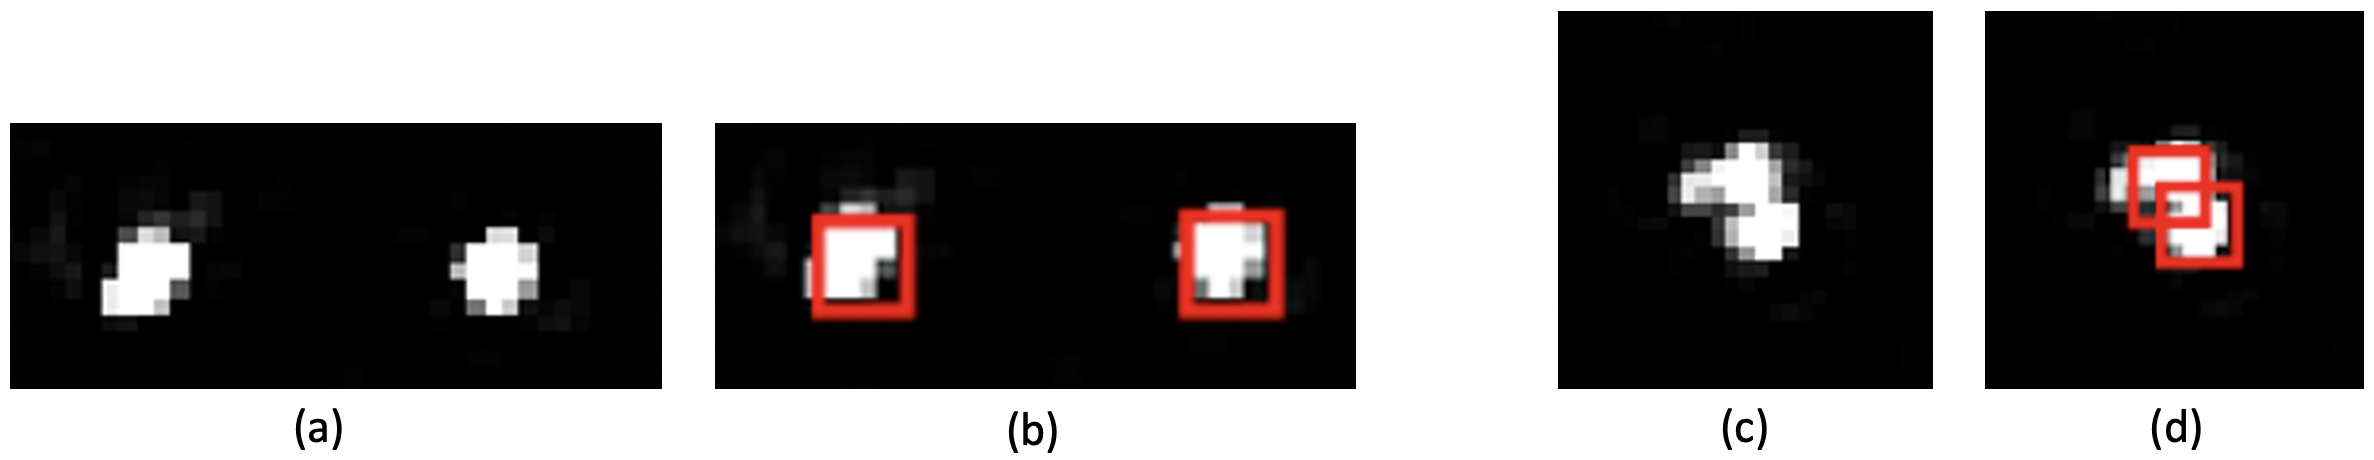
\includegraphics[width=0.3\textwidth]{chapters/wowmom-pmc/figures/peaks.png}
% 	\caption{A zoom-in of two close peaks in Fig. \ref{fig:overall} (b). A clearer understanding of the mechanisms the \imgimg and \yolocust.}
% 	\label{fig:peaks}
% \end{figure}


\subsection{\our vs.\ Prior Works}
\label{subsec:vs_prior}
%%%%%%% comparing 4 $$$$$$$$$$$$

\begin{figure}[t]
	\centering
	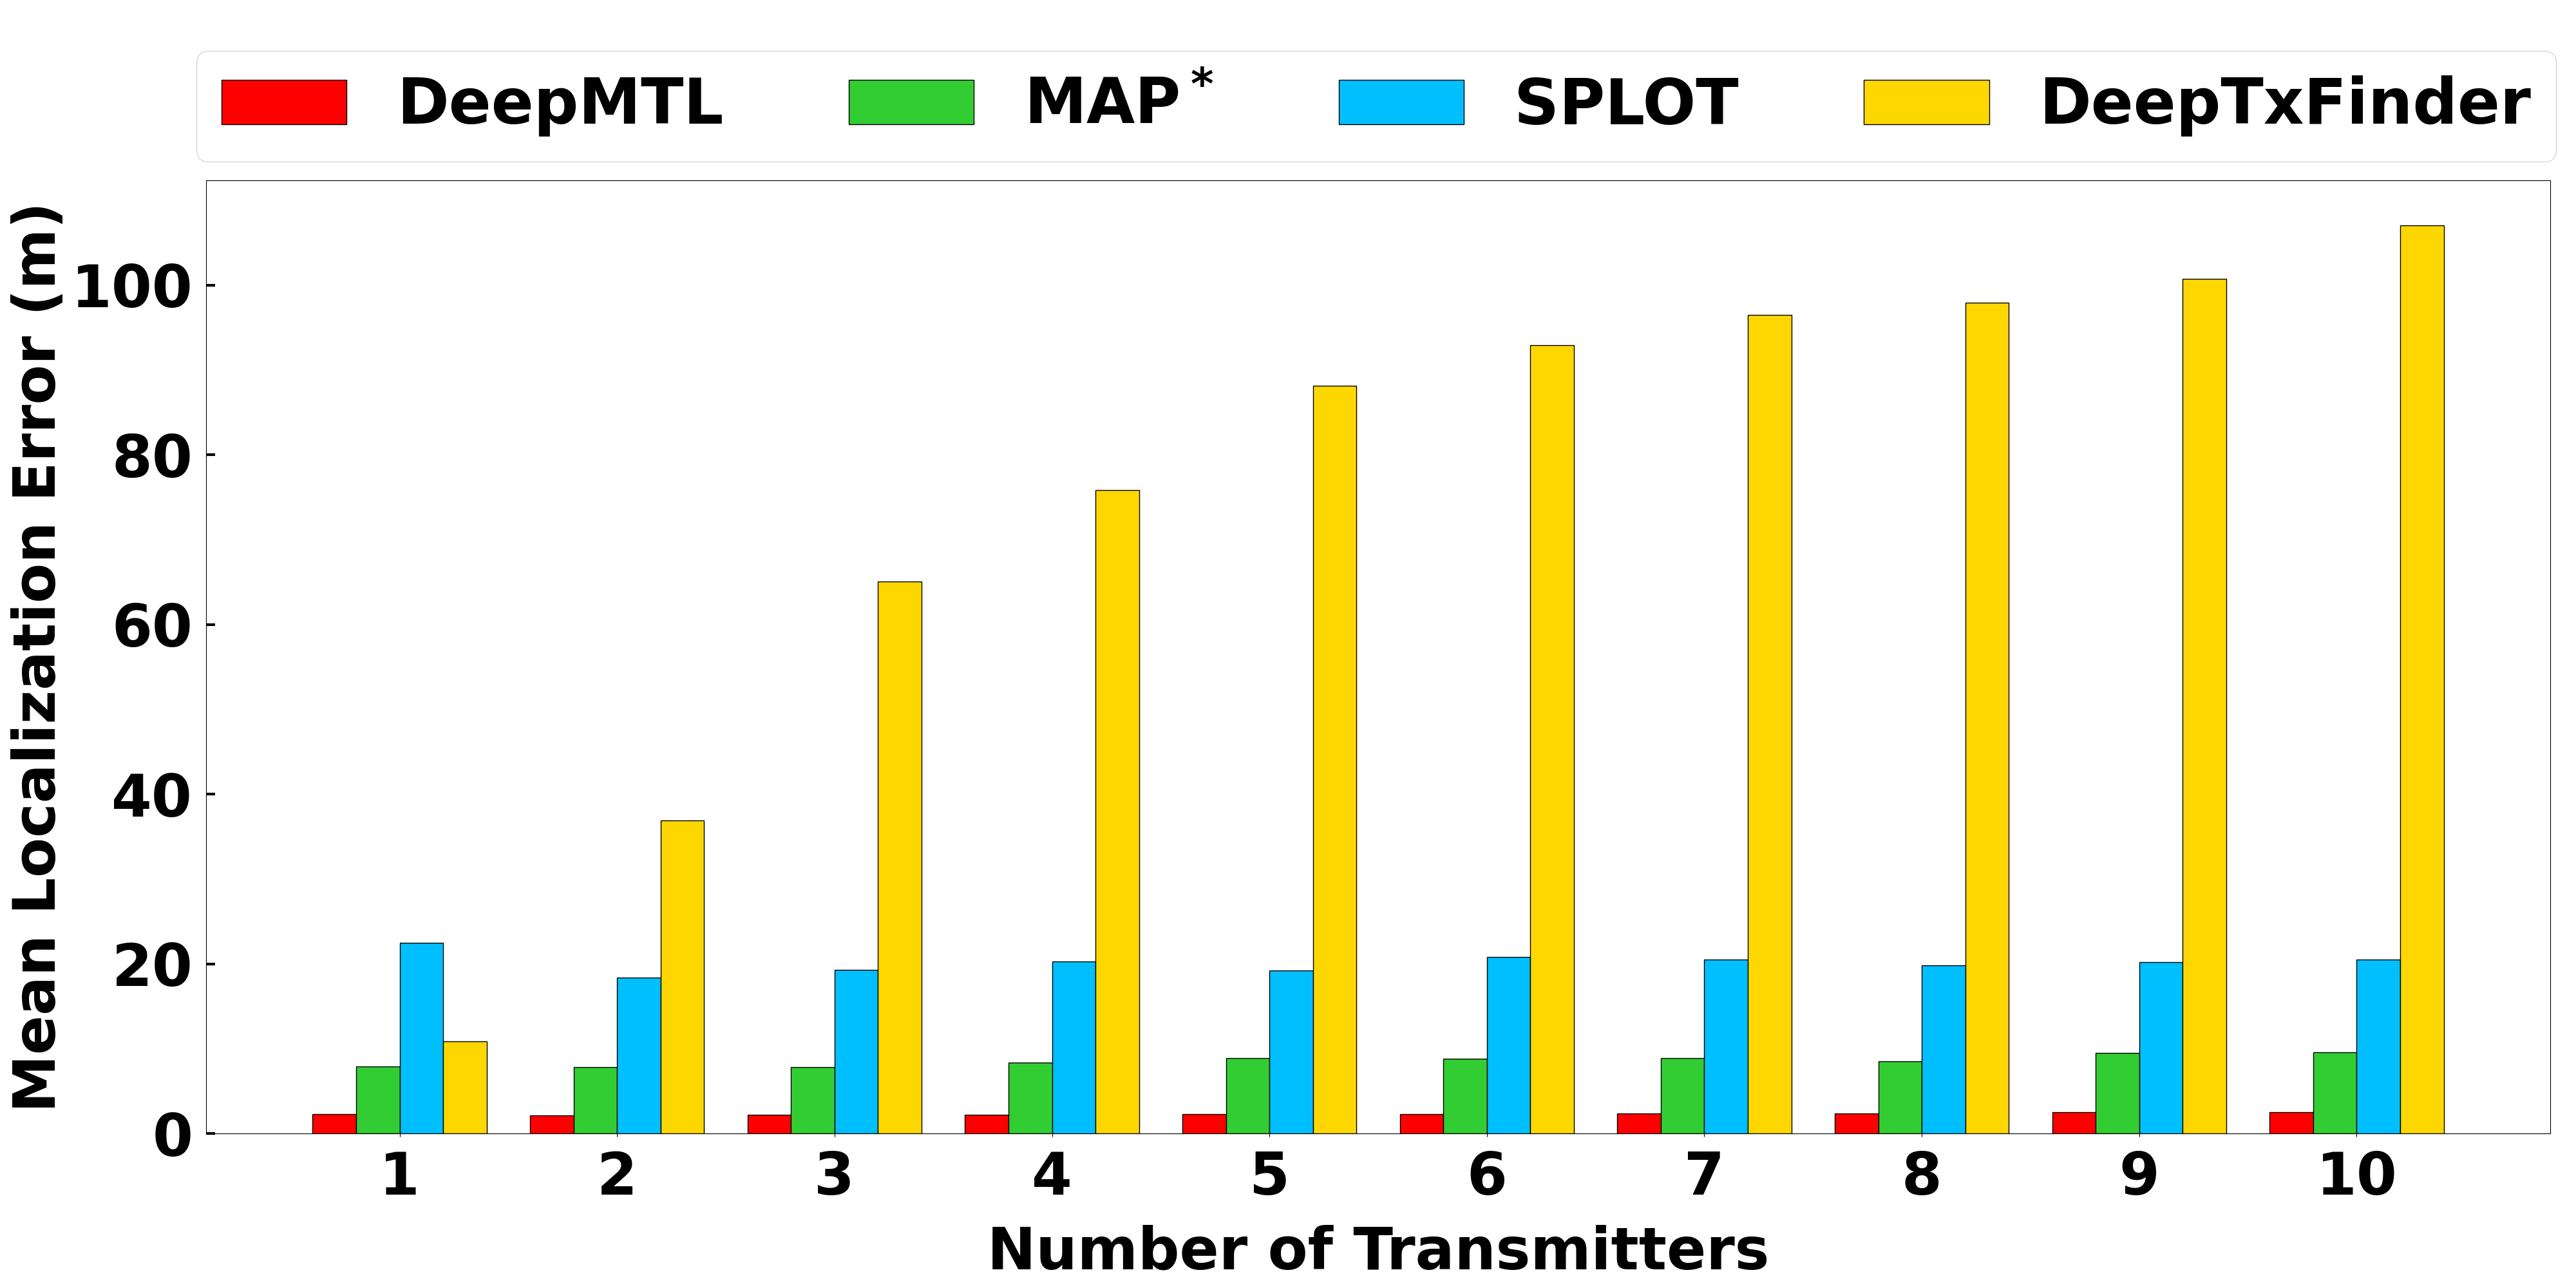
\includegraphics[width=0.75\textwidth]{chapters/wowmom-pmc/figures/log_distance-error_vary_numintru.png}
	\caption{Localization error of \our, \map, \splot, and \deeptx for varying number of transmitters in the log-distance dataset.}
	\label{fig:logdist-error-vary_numintru}
\end{figure}



\begin{figure}[t]
	\centering
	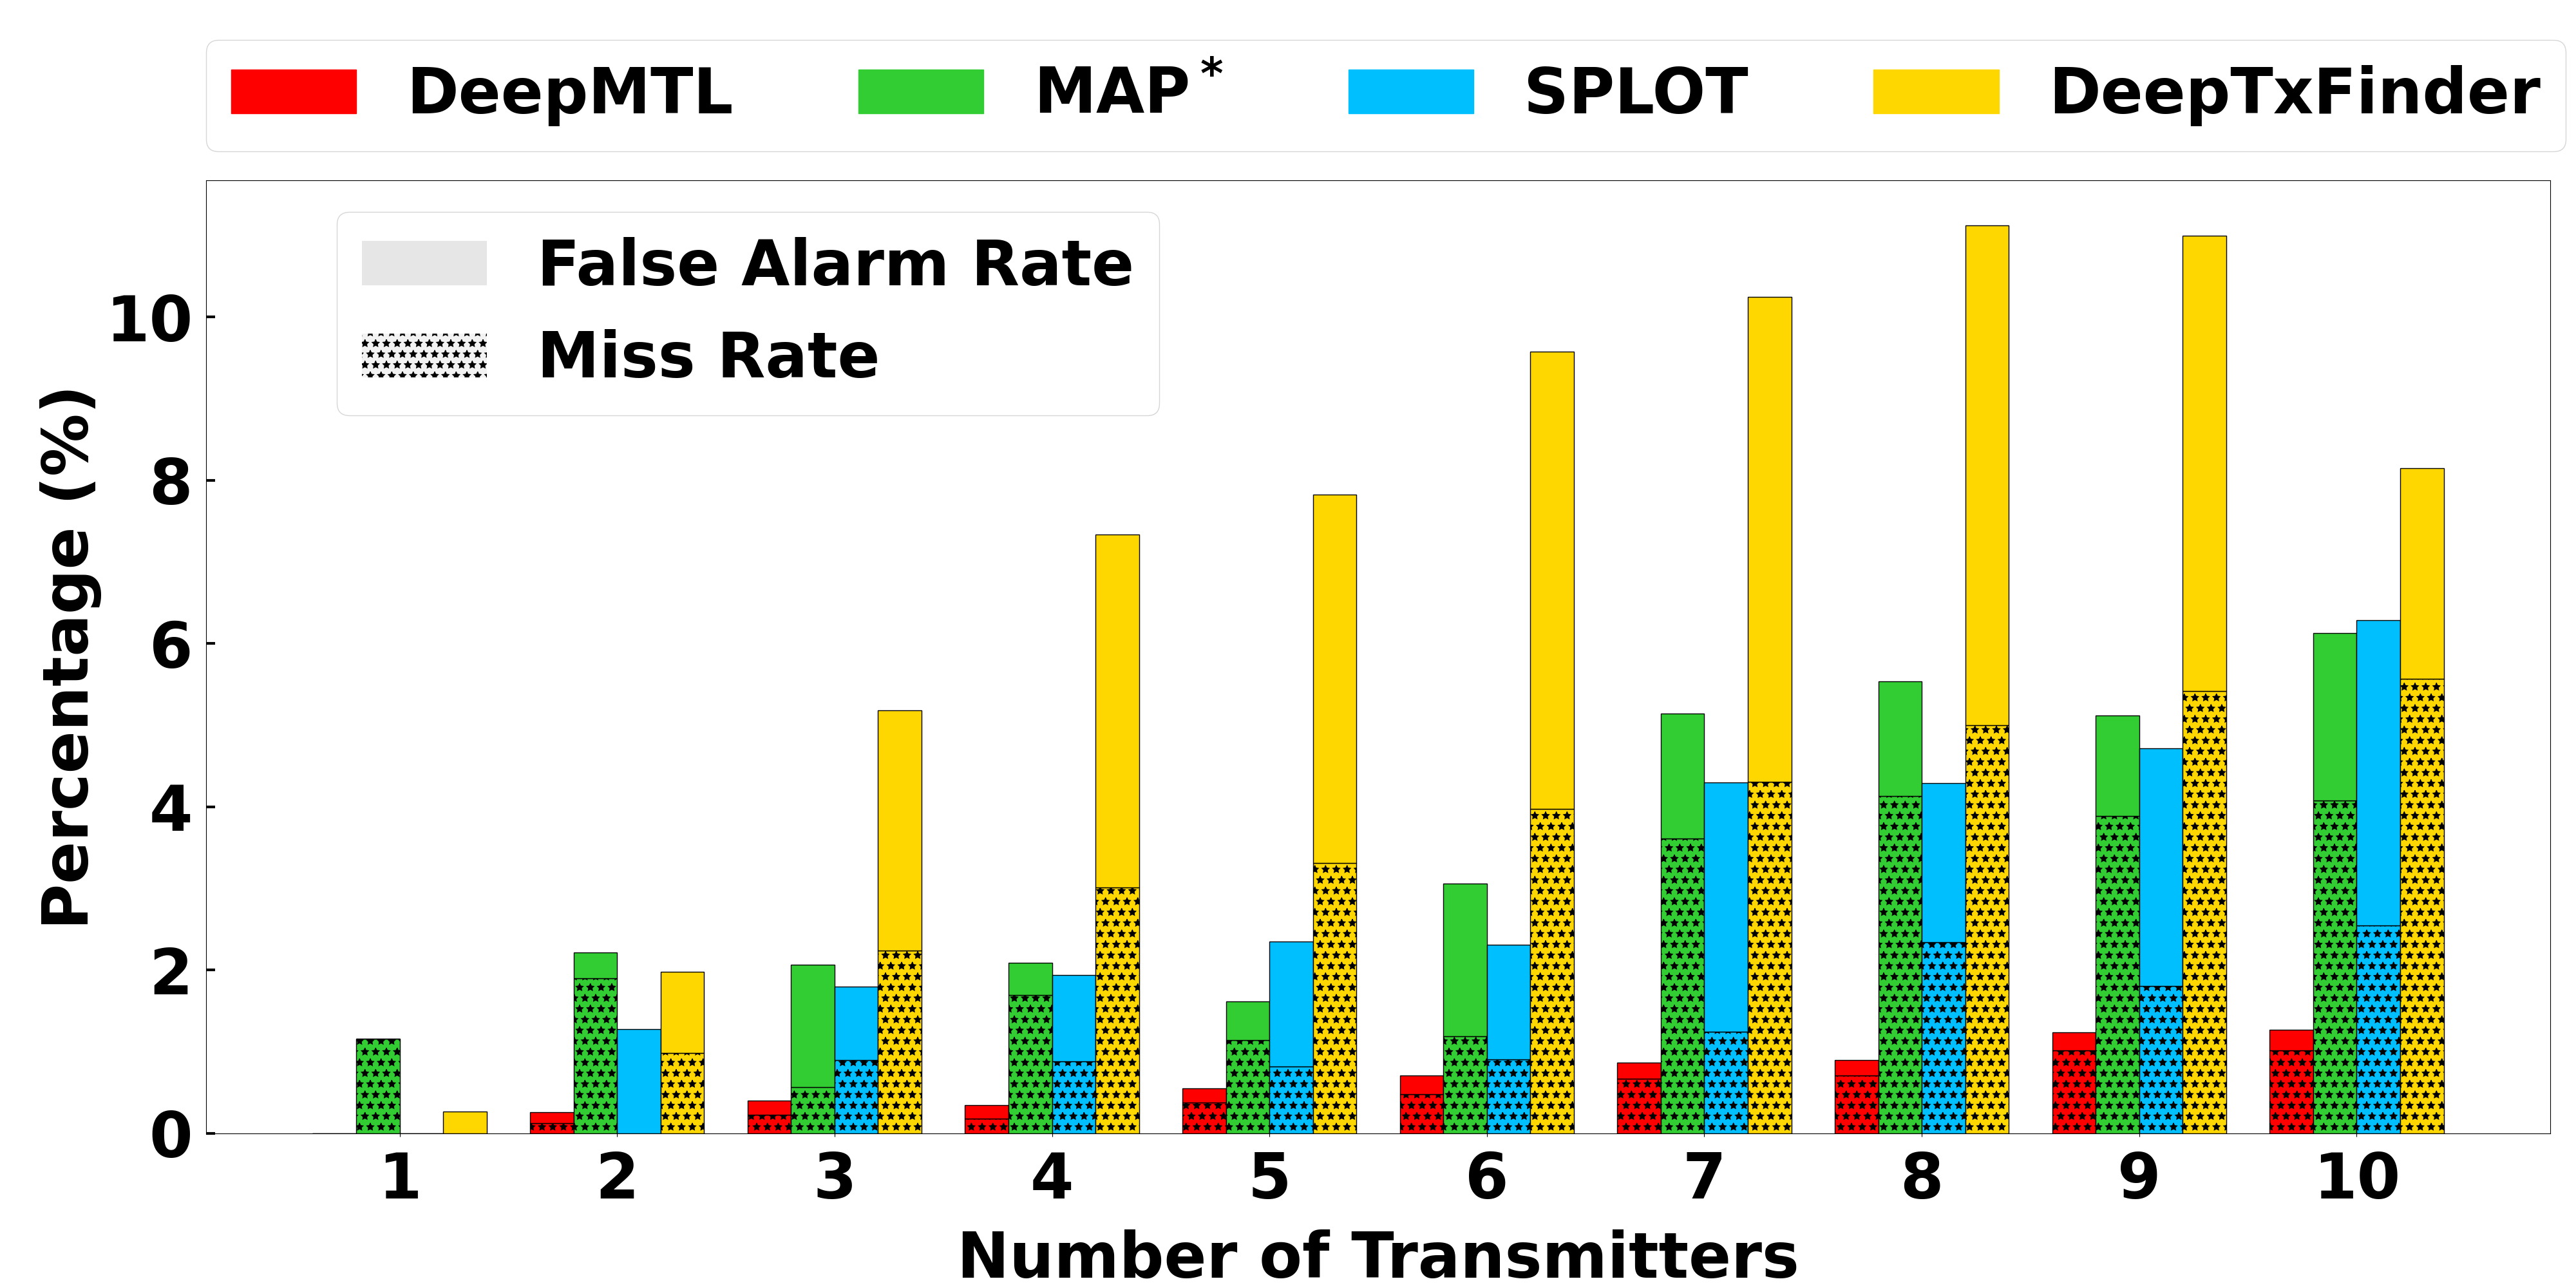
\includegraphics[width=0.75\textwidth]{chapters/wowmom-pmc/figures/log_distance-missfalse_vary_numintru.png}
	\caption{Miss and false alarm rates of \our, \map, \splot, and \deeptx for varying number of transmitters in the log-distance dataset.}
	\label{fig:logdist-missfalse-vary-numintru}
\end{figure}


\begin{figure}[t]
	\centering
	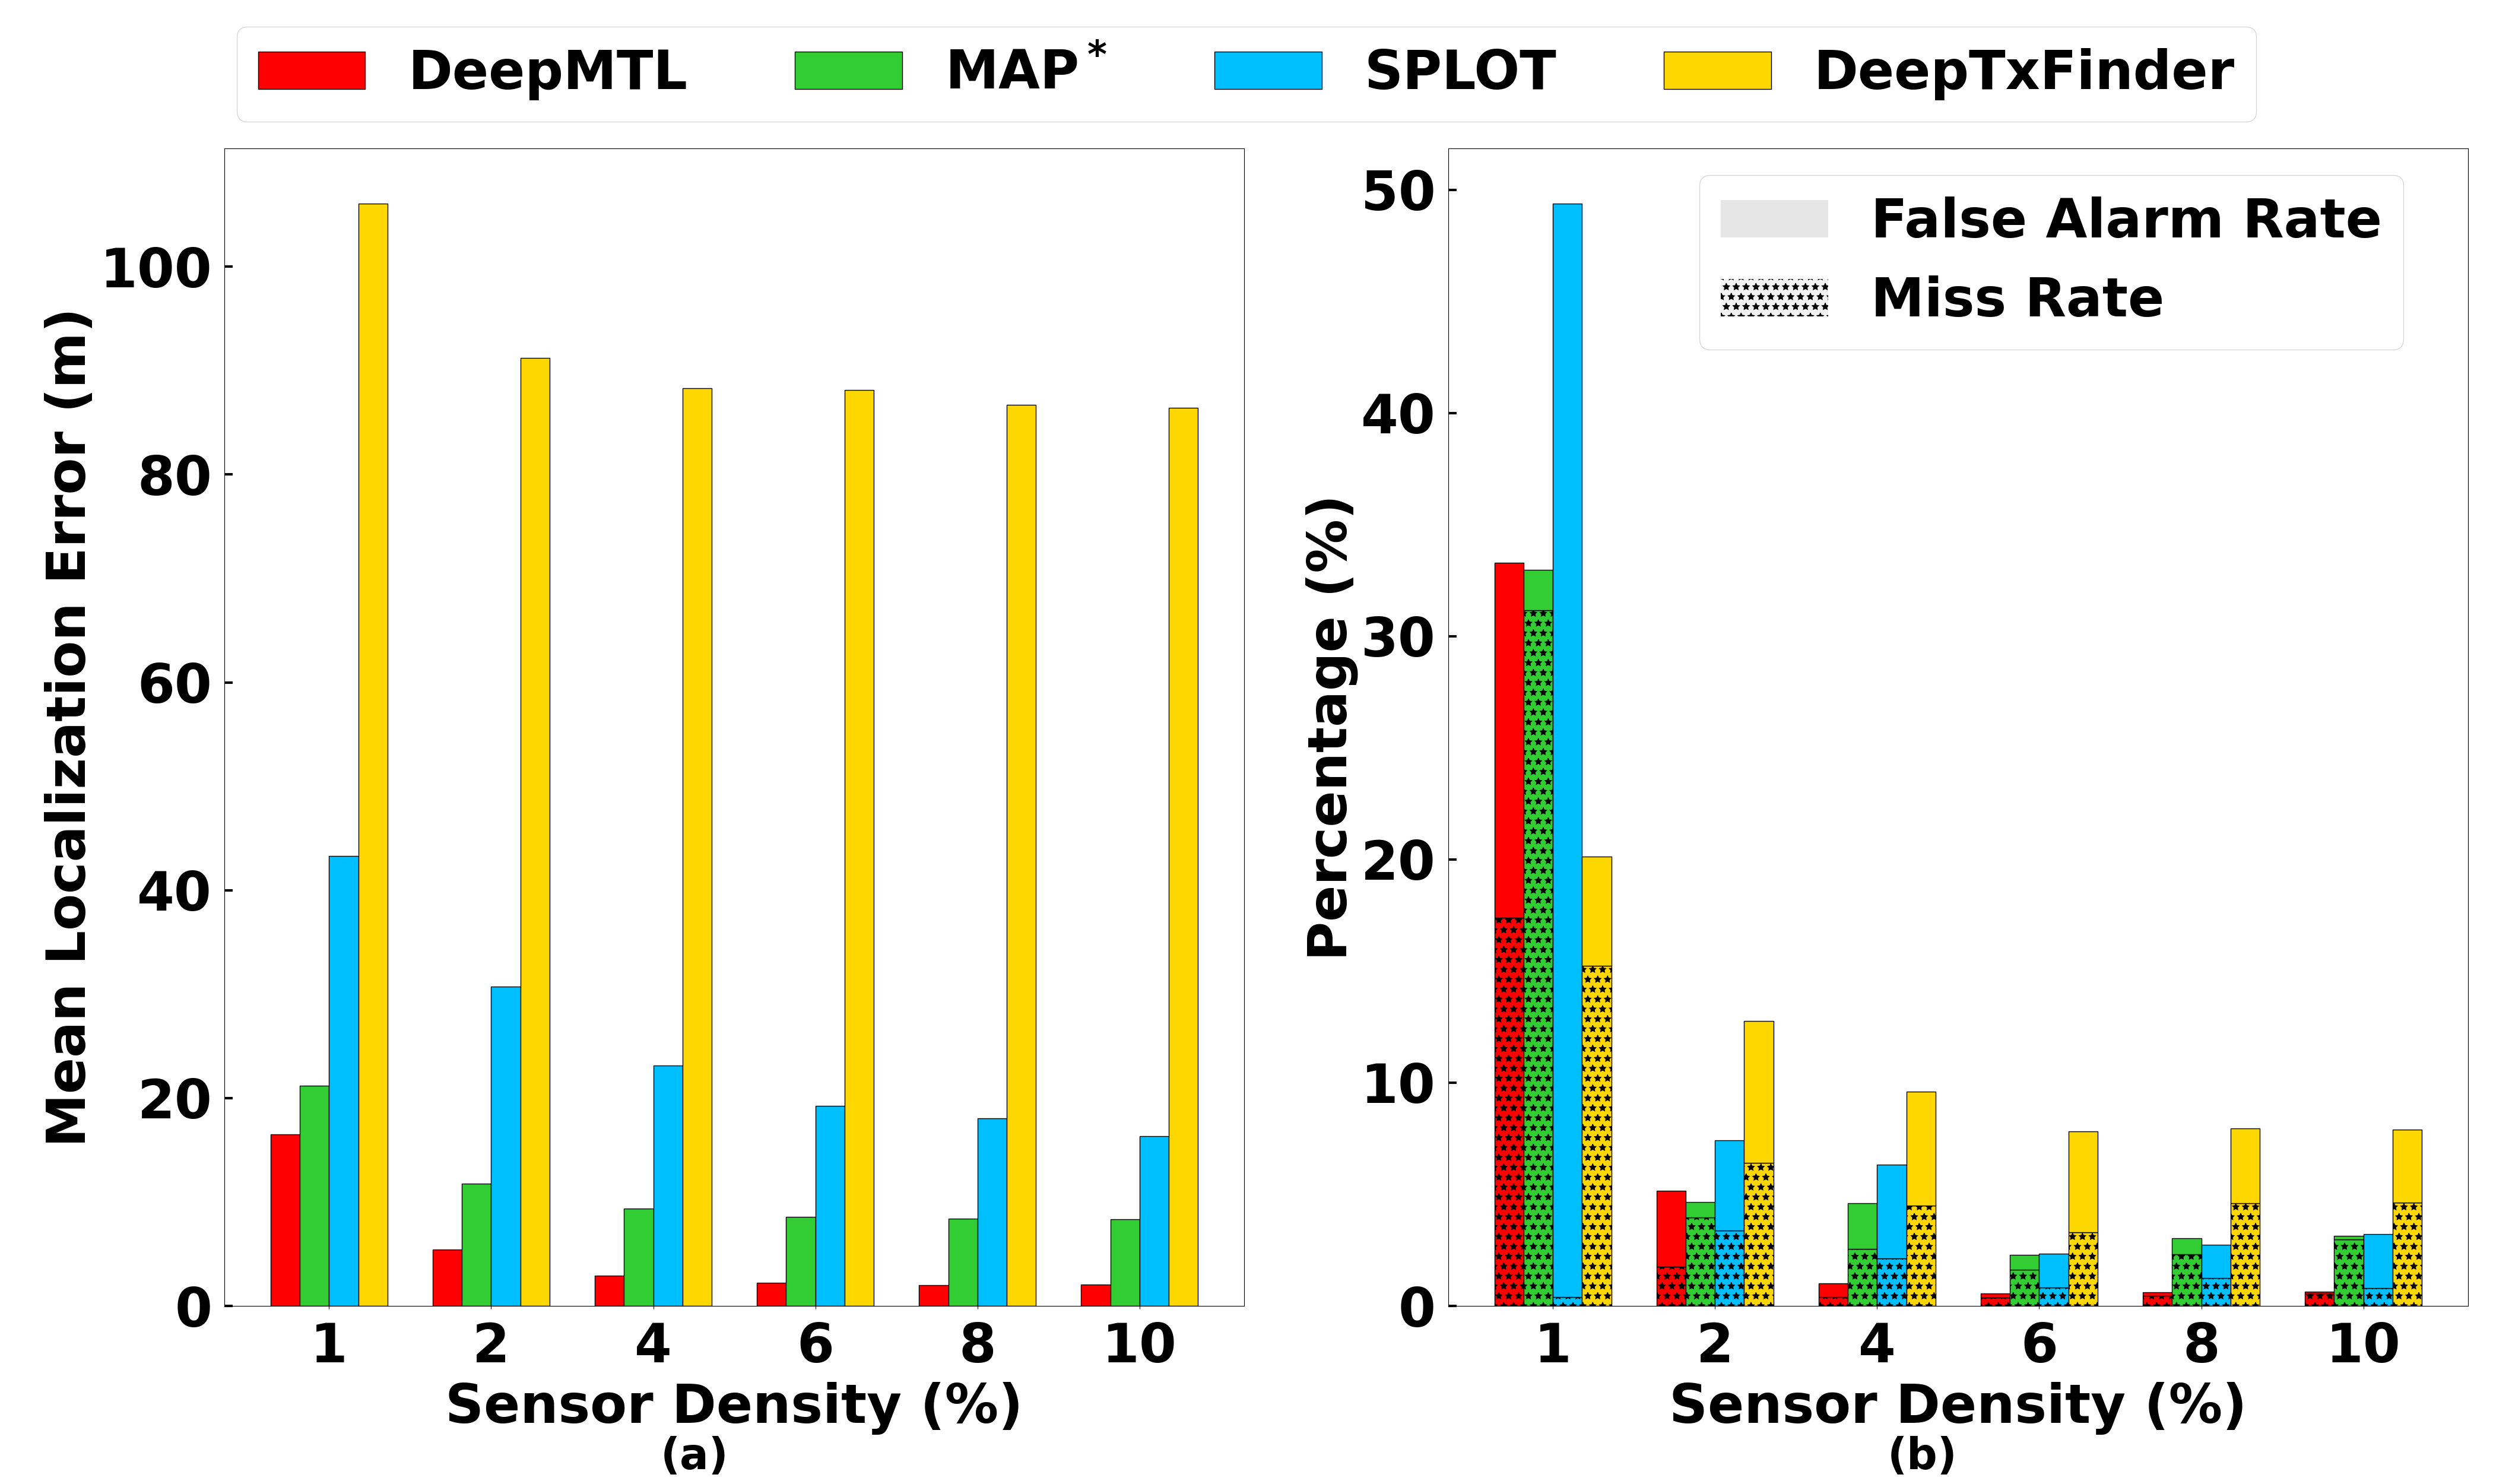
\includegraphics[width=0.75\textwidth]{chapters/wowmom-pmc/figures/log_distance-error_missfalse_vary_sendensity.png}
	\caption{(a) Localization error, and (b) miss and false alarm rates, of \our, \map, \splot, and \deeptx for varying sensor densities in the log-distance dataset.}
	\label{fig:logdist-error_missfalse-vary-sendensity}
\end{figure}





%%%%%%%%%%%%% splat %%%%%%%%%%%%%

\begin{figure}[ht]
	\centering
	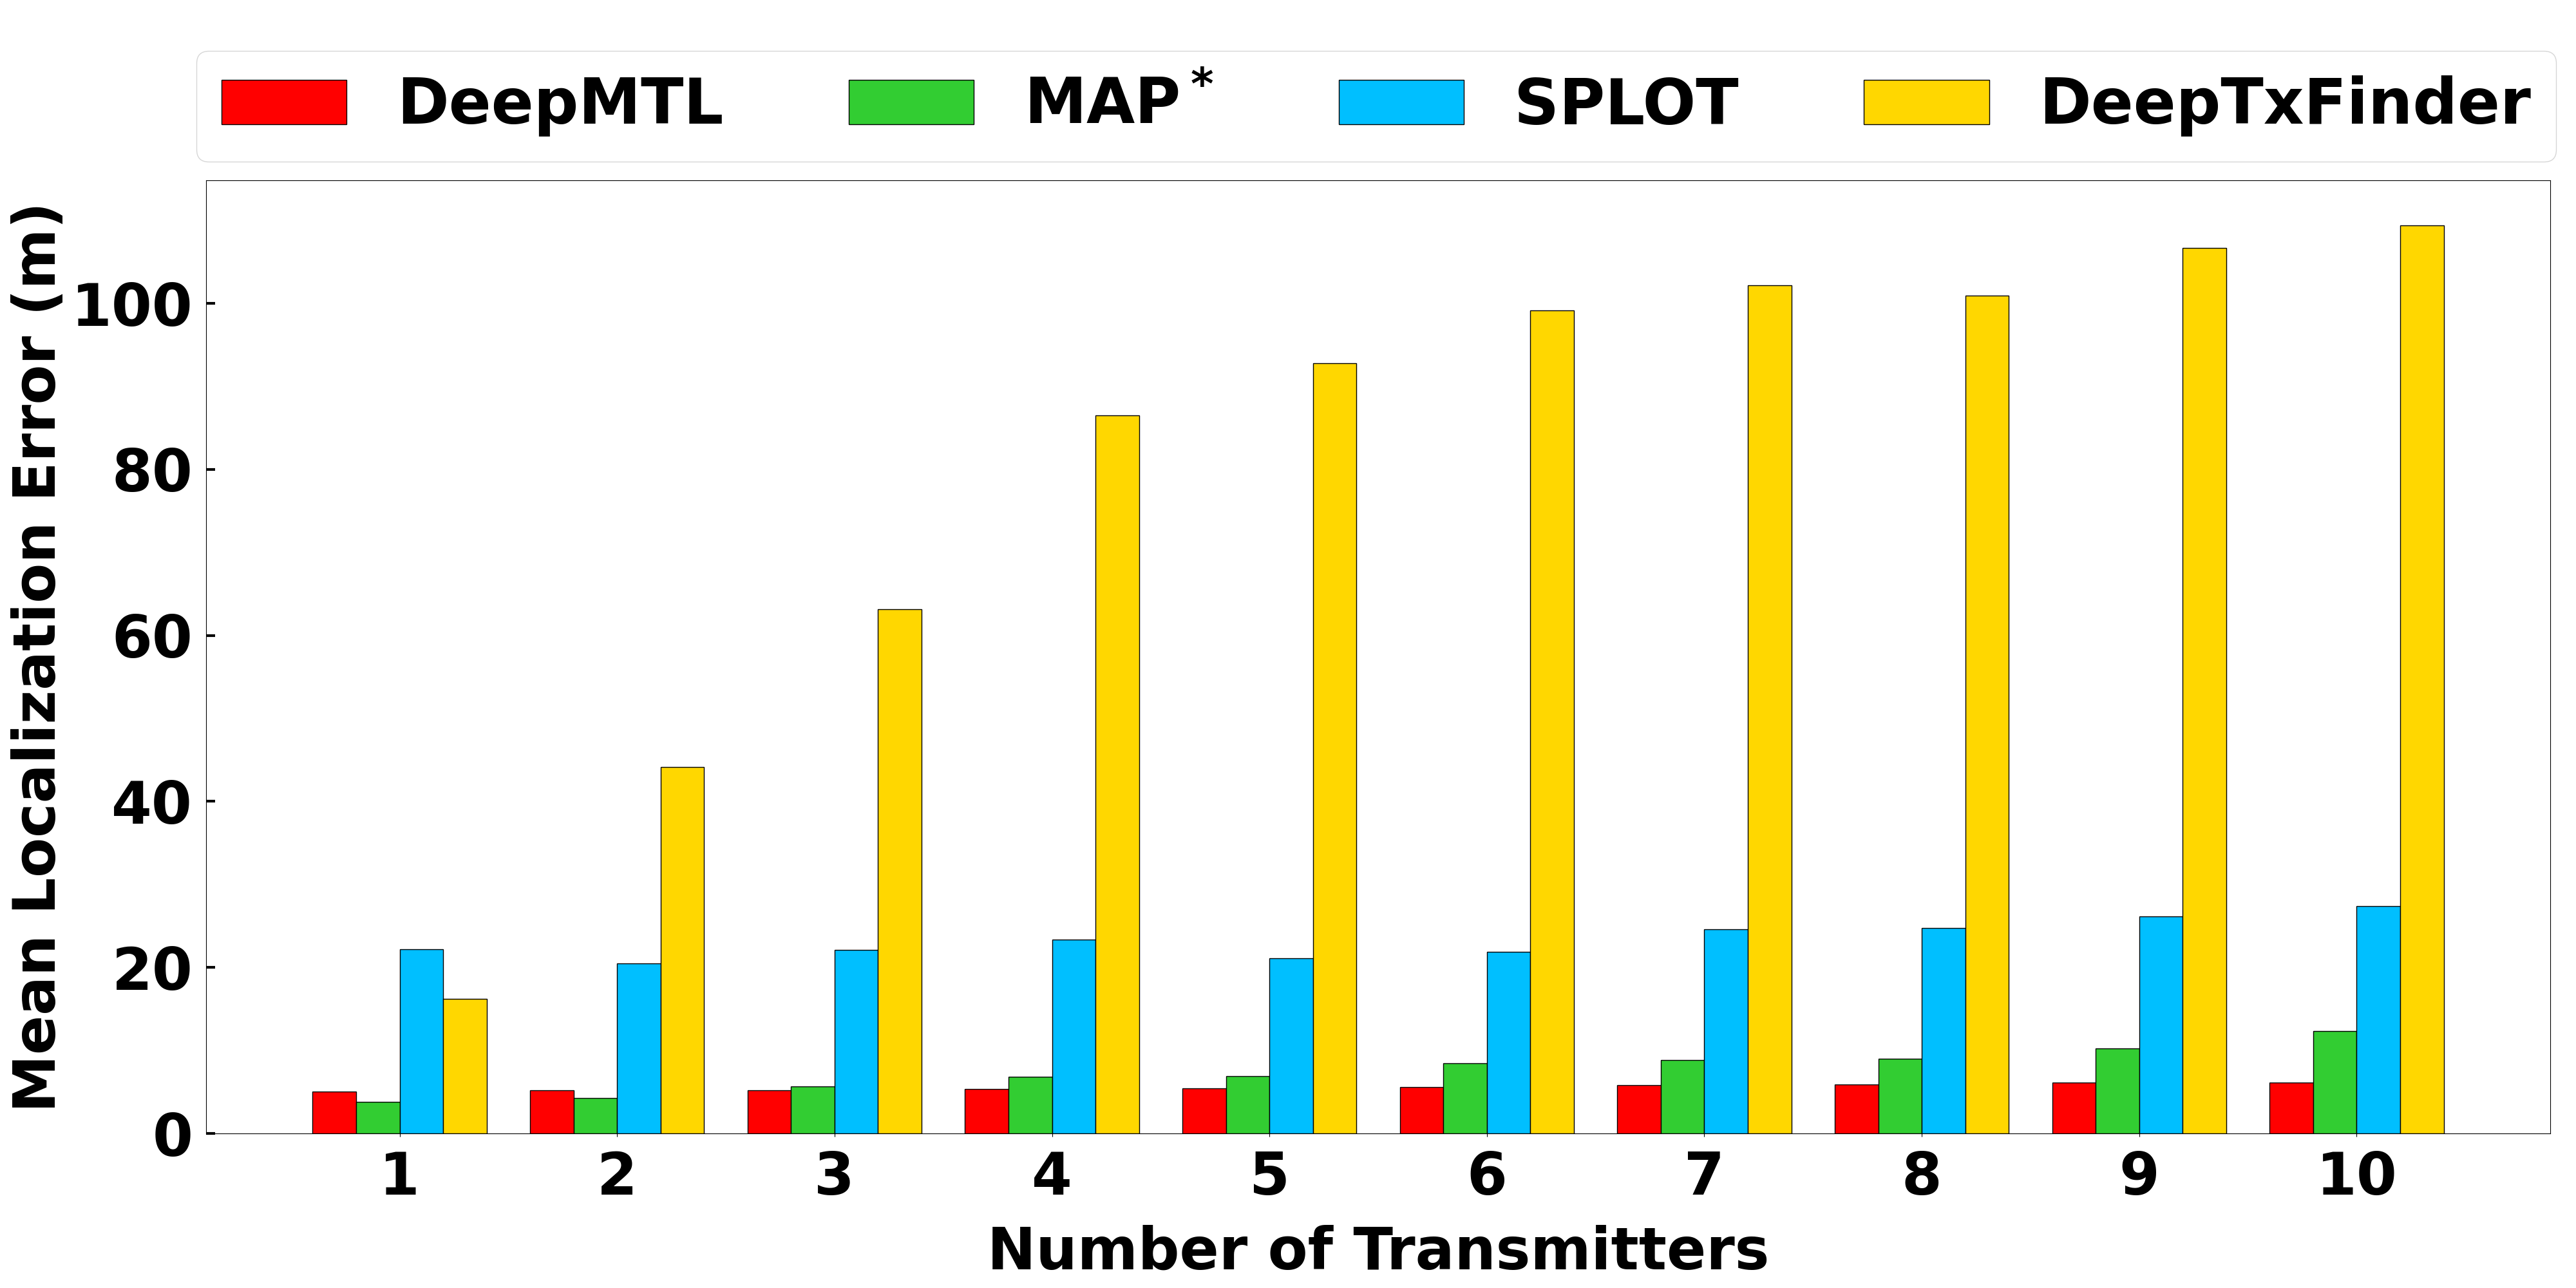
\includegraphics[width=0.75\textwidth]{chapters/wowmom-pmc/figures/splat-error_vary_numintru.png}
	\caption{Localization error of \our, \map, \deeptx and \splot for varying number of transmitters in the SPLAT! Dataset. }
	\label{fig:splat-error-vary_numintru}
\end{figure}

\begin{figure}[ht]
	\centering
	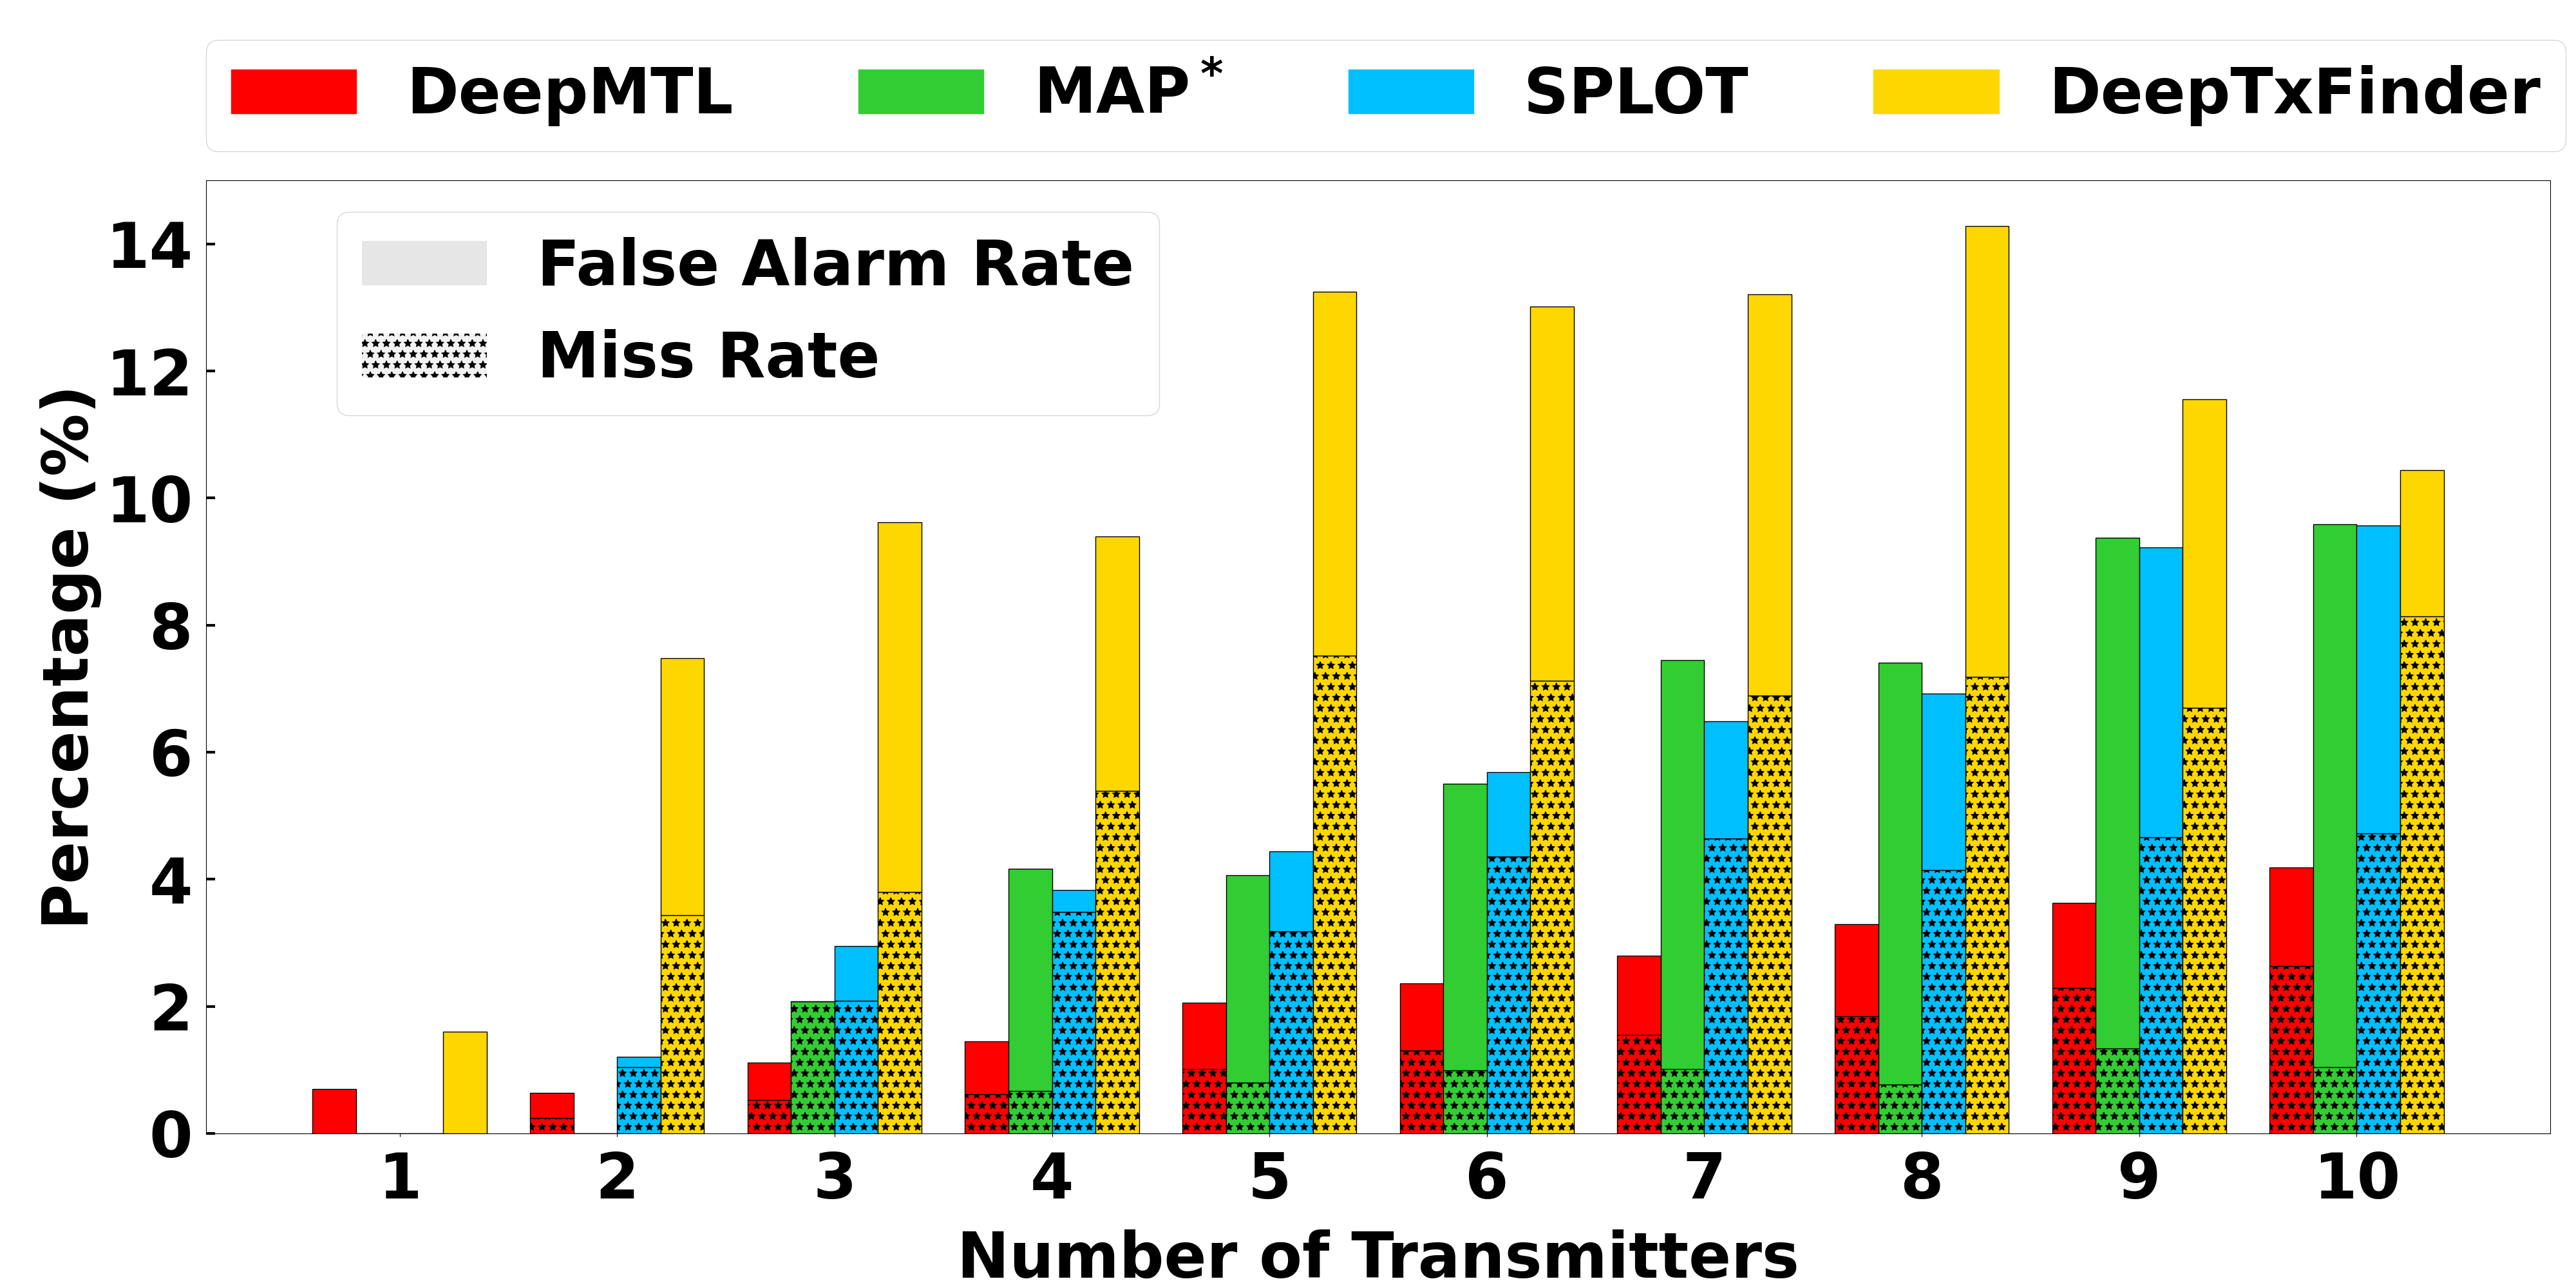
\includegraphics[width=0.75\textwidth]{chapters/wowmom-pmc/figures/splat-missfalse_vary_numintru.png}
	\caption{Miss and false alarm rates of \our, \map, \splot, and \deeptx for varying number of transmitters in the SPLAT! Dataset.}
	\label{fig:splat-missfalse-vary-numintru}
\end{figure}


\begin{figure}[ht]
	\centering
	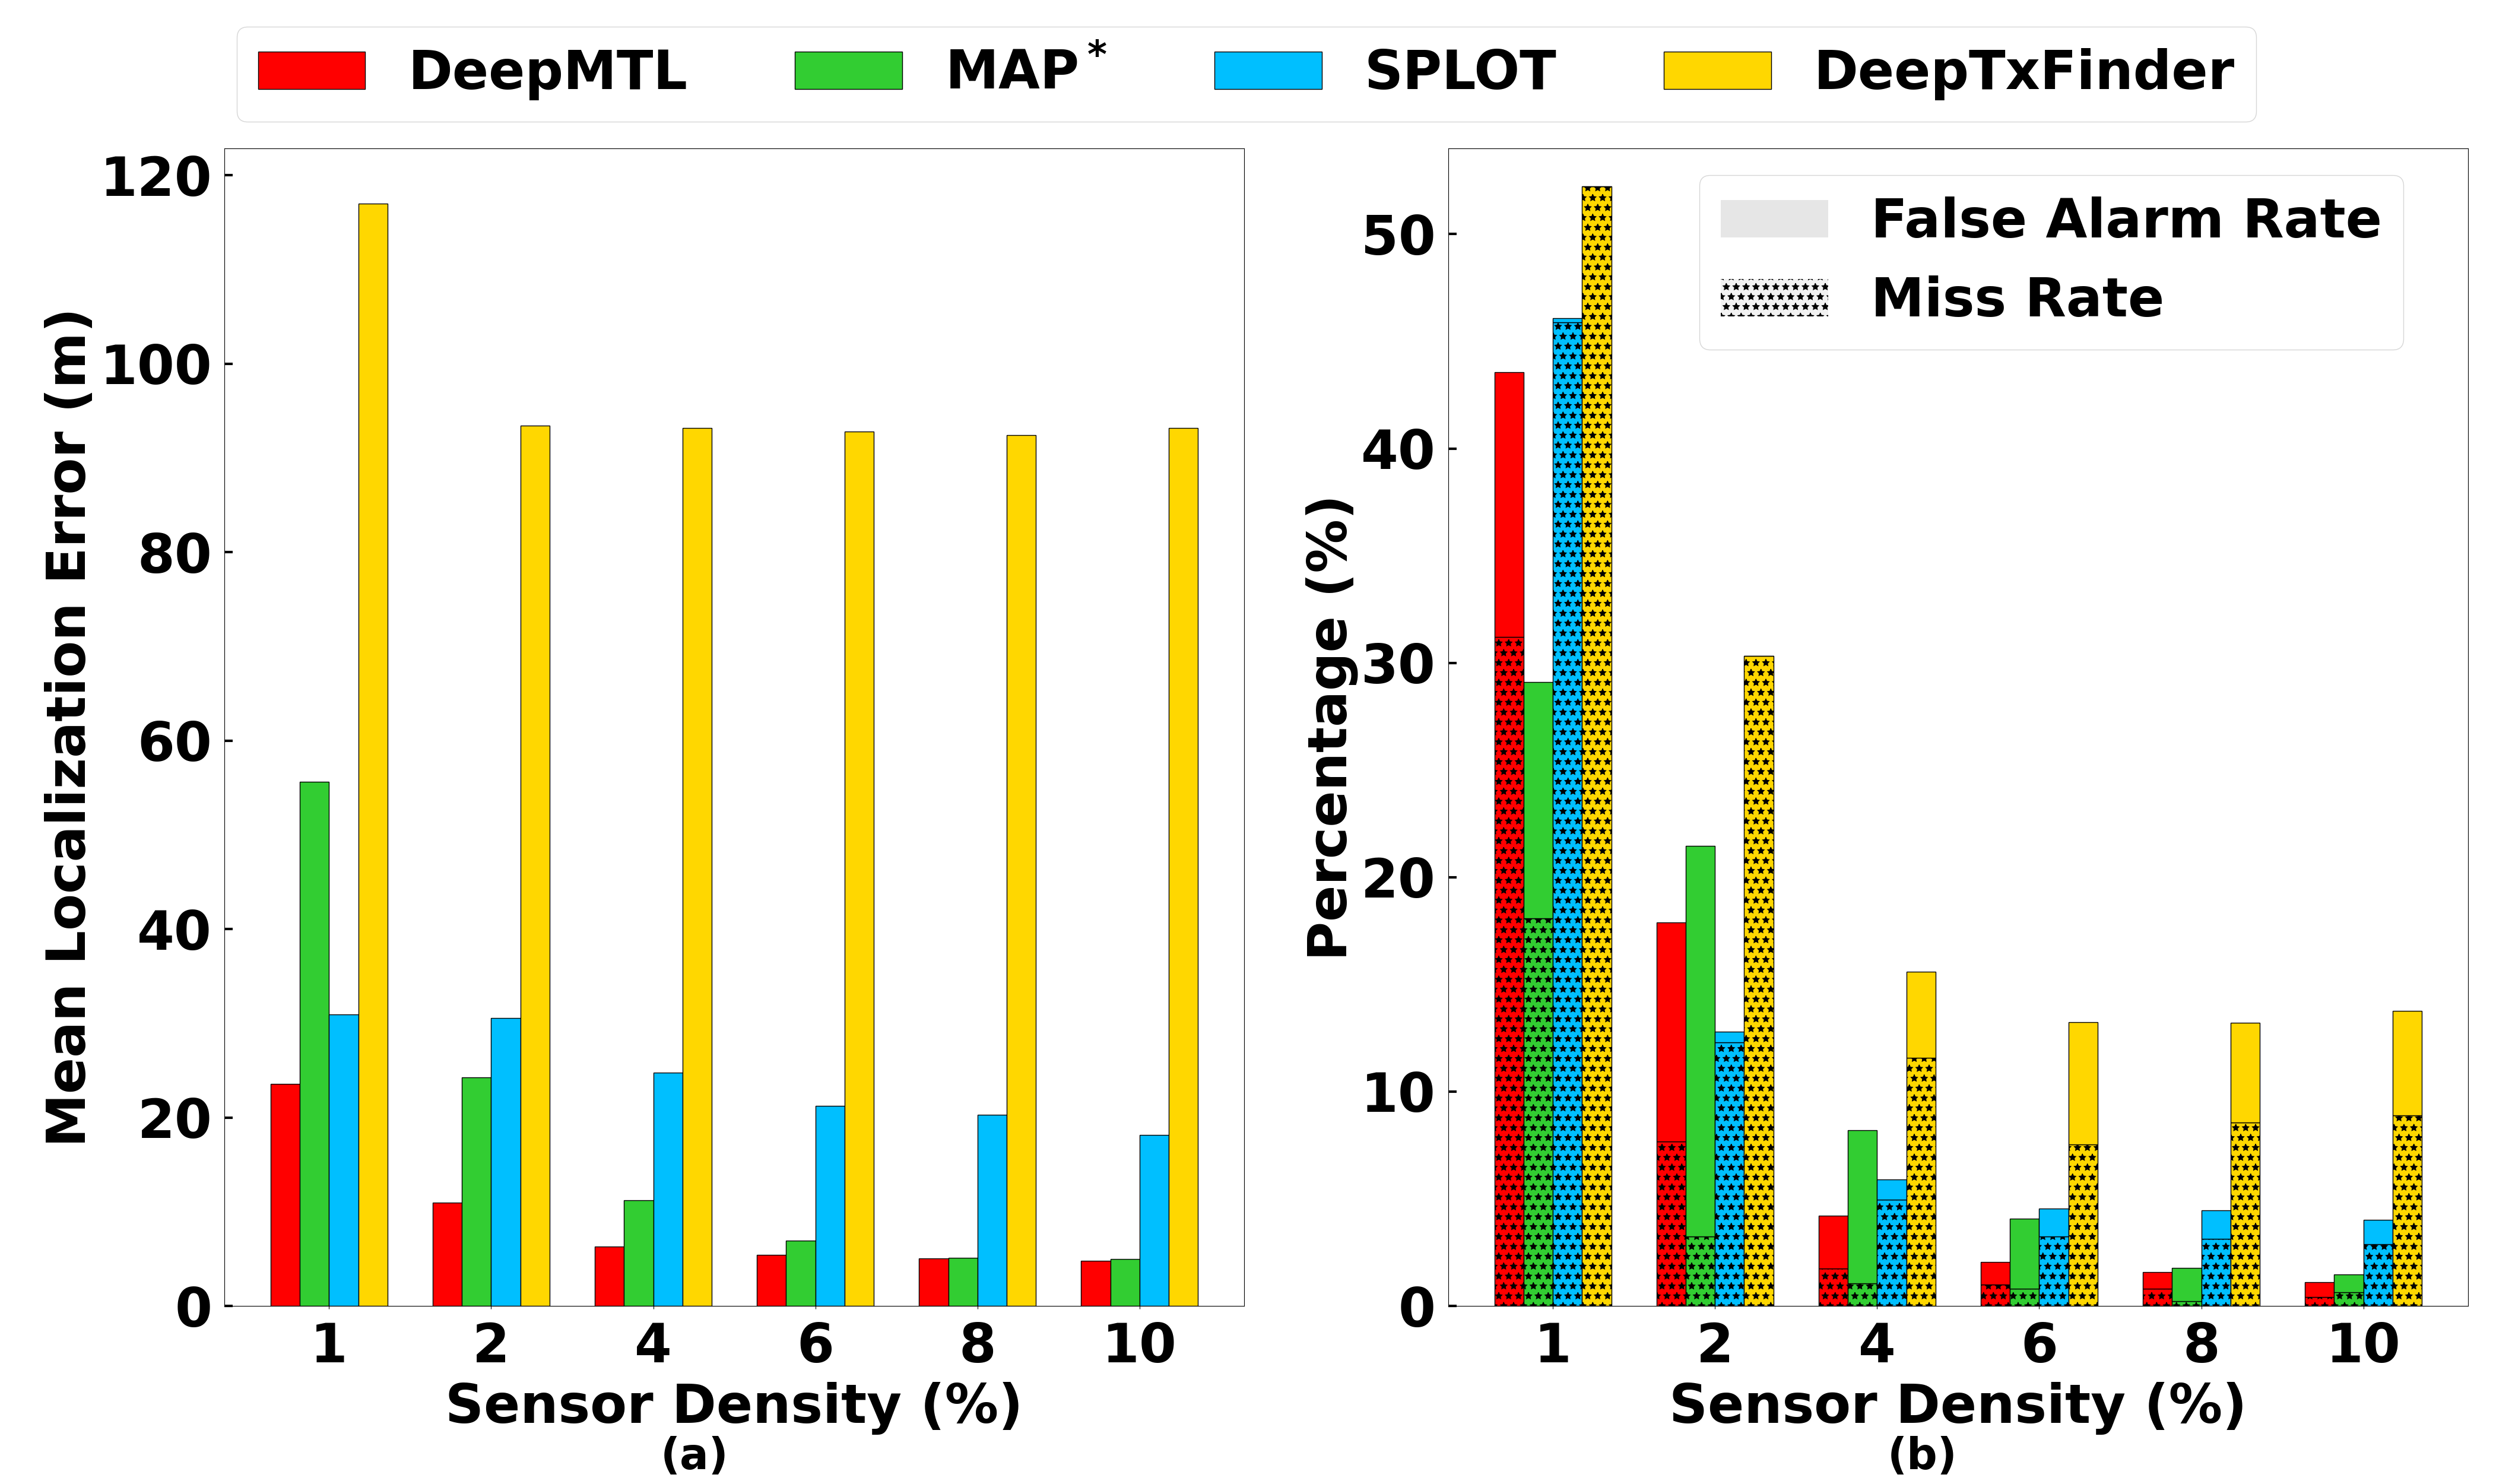
\includegraphics[width=0.75\textwidth]{chapters/wowmom-pmc/figures/splat-error_missfalse_vary_sendensity.png}
	\caption{(a) Localization error, and (b) miss and false alarm rates, of \our, \map, \splot, and \deeptx for varying sensor densities in the SPLAT! Dataset.}
	\label{fig:splat-error-vary-sendensity}
\end{figure}



In this subsection, we compare \our with \splot, \map, \deeptx in both log-distance (Fig.~\ref{fig:logdist-error-vary_numintru}, \ref{fig:logdist-missfalse-vary-numintru}, \ref{fig:logdist-error_missfalse-vary-sendensity}) and SPLAT (Fig.~\ref{fig:splat-error-vary_numintru}, \ref{fig:splat-missfalse-vary-numintru}, \ref{fig:splat-error-vary-sendensity}) propagation models and thus, datasets.
We observe similar performance trends for both datasets, i.e., 
\our significantly outperforms the other approaches by a large margin (in many cases, by more
than 50\% in localization errors, false alarms, and miss rates). For all techniques, as expected,
the performance is generally worse in the SPLAT dataset compared to the log-distance dataset.
%%%%%%%%%%%%%%%%

\softpara{Varying Number of Transmitters.}
Fig.~\ref{fig:logdist-error-vary_numintru} and Fig.~\ref{fig:splat-error-vary_numintru} show the localization error with varying number of transmitters, in the two datasets. We see that \our has a mean localization error of only 2 to 2.5 meters (roughly, one-fourth of the side length of a pixel/grid cell) in the log-distance dataset and about 5 to 6 meters in the SPLAT dataset. In comparison, the
localization errors of \map, \splot, \deeptx are two to three times, eight to nine times, and 
few tens of times respectively more than that of \our. 
%%%%%%%%%%%%%%%%%%%%%%%%%%%%%%%%%%%%%%%
Fig.~\ref{fig:logdist-missfalse-vary-numintru} and Fig.~\ref{fig:splat-missfalse-vary-numintru} show the miss and false alarm rates with varying number of transmitters in the two datasets.
We observe that \our's summation of miss and false alarm rate is only 1\% even at 
ten transmitters in the log-distance dataset, and about 4\% for the case of \splat dataset. 
In comparison, the summation of miss and false alarm rates for other schemes is at least 6\% and
10\% respectively for the two datasets, when there are ten transmitters.

\softpara{Varying Sensor Density.}
Fig.~\ref{fig:logdist-error_missfalse-vary-sendensity} and Fig.~\ref{fig:splat-error-vary-sendensity} plot the performance of various algorithms for varying sensor density in the two datasets. For very low sensor density of 1\%, all algorithms perform 
badly (in comparison with higher sensor densities), but \our still performs the best except that \map performs best at 1\% in terms of false alarm rate and miss rate.
For higher sensor densities, we observe a similar performance trend as above---i.e., \our easily outperforms the other schemes by a large margin.
For the SPLAT! dataset at the 6\% sensor density, the summation of false alarm rate and miss rate is 2\%, which is higher than the 1\% summation for the log-distance dataset.

\softpara{Running Times.}
The run time of \our (in tens of milliseconds) is orders of magnitude faster than \map and \splot (both in seconds). 
See Table \ref{table:running-time}. 
The \our run time is an order of magnitude slower than \deeptx (in a few milliseconds), due to the deep \yolocust taking up over 90\% of the run time.


\softpara{Summary and Analysis}. 
In summary, our approach significantly outperforms the other approaches in all the accuracy performance metrics, as well as in terms of latency. 
In particular, our approach also significantly outperforms the other CNN-based approach \deeptx. 
The main reason for \deeptx's inferior performance is its inability to accurately predict the number of TXs---which 
forms a fundamental component of their technique. In contrast, \our can circumvent explicit pre-prediction
of number of transmitters by using a well-developed object-detection technique which works well for multiple objects 
especially in our context of simple objects.
%%%%%%%%%


%\blue{We observe \deeptx is performing bad mainly because it cannot predict the number of the TX accurately. 
%The inaccuracy in predicting the number of TX will later affect predicting the location of TX negatively. 
%The advantage here for \our is that the \yolocust is able to take care of the multiple transmitters elegantly through advanced %computer vision techniques. 

%Note that we tried to enhance the CNN model that predicts the number of TX. 

%The overall performance increases but the improvement is not significant. The superiority of \our over \mtl and \splot is because of reframing the wireless localization problem to an image-based problem and resorting to computer vision techniques.}

%how that our approach outperforms the previous approaches 
%significantly (by 50\% or more) in accuracy performance metrics, and incurs an order of magnitude
%less latency compared to other prior works. 

%\begin{enumerate}
%    \item [8 PLOTS] Large scale simulations (100 by 100). Log-distance (?) and Splat. 100 to 1000 sensors (one model). 1 to 10 TXs. Power Range: p plus/minus 5 dB (maybe, plus/minus 10 dB later). PLOTS: Varying # of TXs, # of sensors, # of training images (10k, 20k, 50k, 75k, 100k).
%    \item [4 PLOTS] Testbed Data. IPSN 2020. 1 to 3 TXs. .....   
%    \item Algorithms: Ours (2), IPSN 20, SPLOT, DeepTxFinder.
%    \item Need to bring in training cost comparison across algorithms.
%\end{enumerate}

% \subsection{Large Scale Simulation Dataset}
% Here we simulate the training dataset through a propagation model.


% \subsection{Small Scale Trace Driven Dataset}
% Although simulation is a good metric to pick the best localization algorithm, the better setting is a miniature but realistic experiment using commercial devices.
% Here we use data collected from \cite{ipsn20-mtl} (outdoor). The reason we pick this dataset is it reflects a realistic application of share spectrum system and it gives us the power to change the TXs' configuration (location and power) as it basically provides path-loss values between any arbitrary pair of locations.
% This dataset was collected in area of $32m \times 32m$ with 100 grid cells (each of $3.2m \times 3.2m$).
% We vary number of intruders, deployed sensors, and the number of training samples just what we did for simulations.

% \softpara{Varying Number of Intruders.} We see a similar trend compared to simulations as Figure [] shows. We vary the number of intruders between ... and ...
% We can see that \yolo and \peak can outperform the other algorithms, overall.
% When the number of intruders increases, the performance of the algorithms ....
% As expected, false alarm and miss rate values show that ... has the worst performance while ... shows its strength.
% The performance of ..., among all, shows a consistent behavior meaning ... 


% \softpara{Varying Sensor Density.}
% Now, we try to understand the importance of deployed sensors density.
% We change, due tho small area of interest, from very low number ... to the number as high as ...
% Figure [] simply proves that the higher the number of sensors, the better results we can get for all algorithms.

% \softpara{Varying Training Cost.}
% Finally, we consider the effect of number of training samples on the efficiency of the described algorithms. See Figure [].
% Performance of all algorithms get better when the number of training samples increases. ... performs better when the training samples size is small but ... get much more benefit when this value is moderate.


\subsection{Transfer Learning}
\label{subsec:transfer_learning}

\begin{figure*}[t!]
    \centering
    \begin{subfigure}[t]{0.48\textwidth}
        \centering
        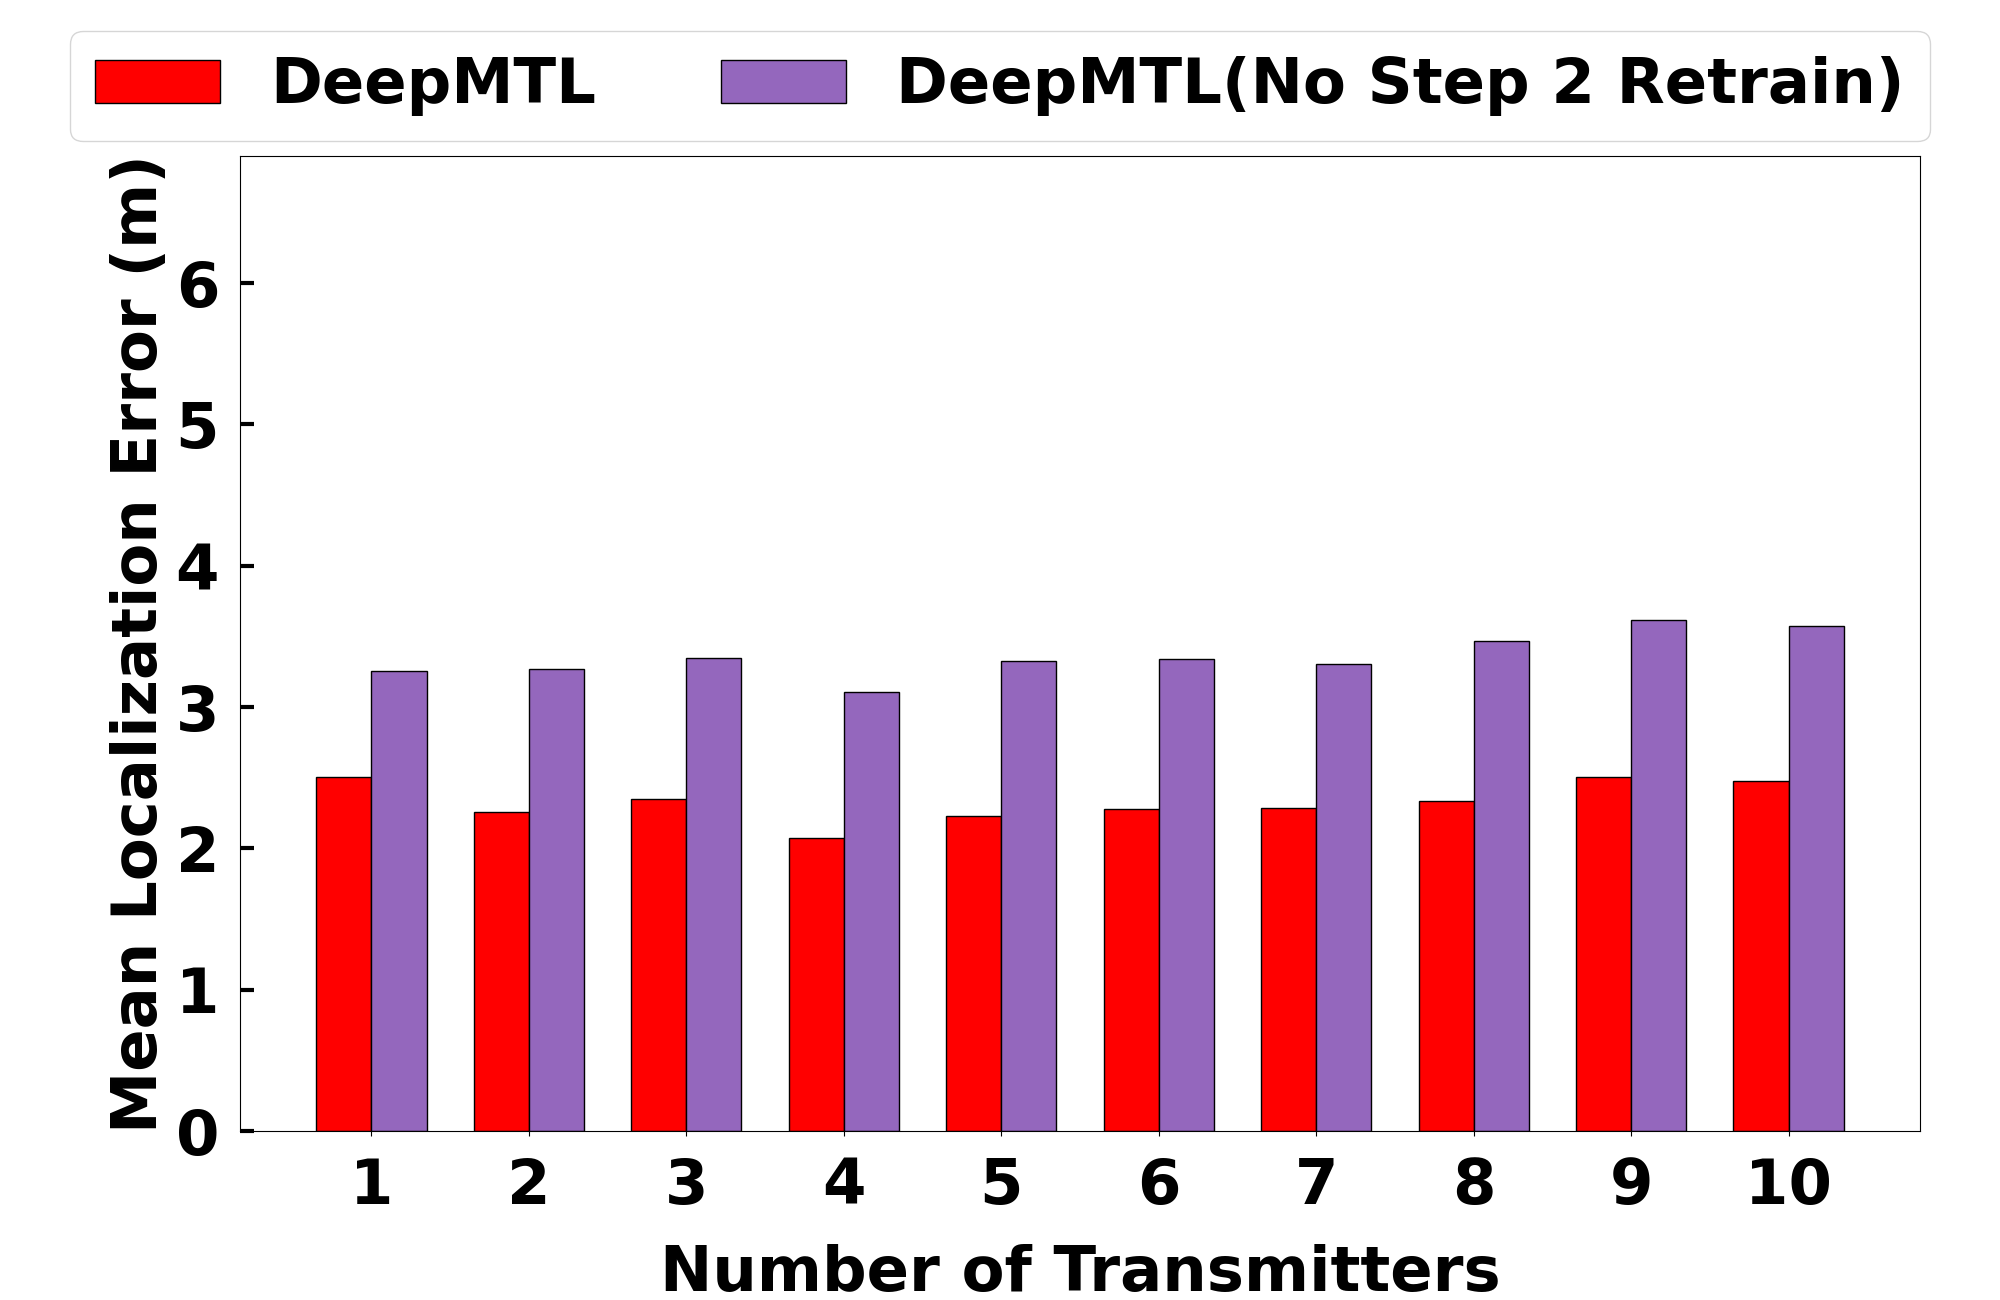
\includegraphics[width=\textwidth]{chapters/wowmom-pmc/figures/noretrain-logdistance-error-vary_numintru.png}
        \caption{First step trained in log-distance data, while the second step trained in SPLAT! data. Tested on the log-distance data.}
        \label{fig:notrain-logdist}
    \end{subfigure}%
    ~
    \begin{subfigure}[t]{0.48\textwidth}
        \centering
        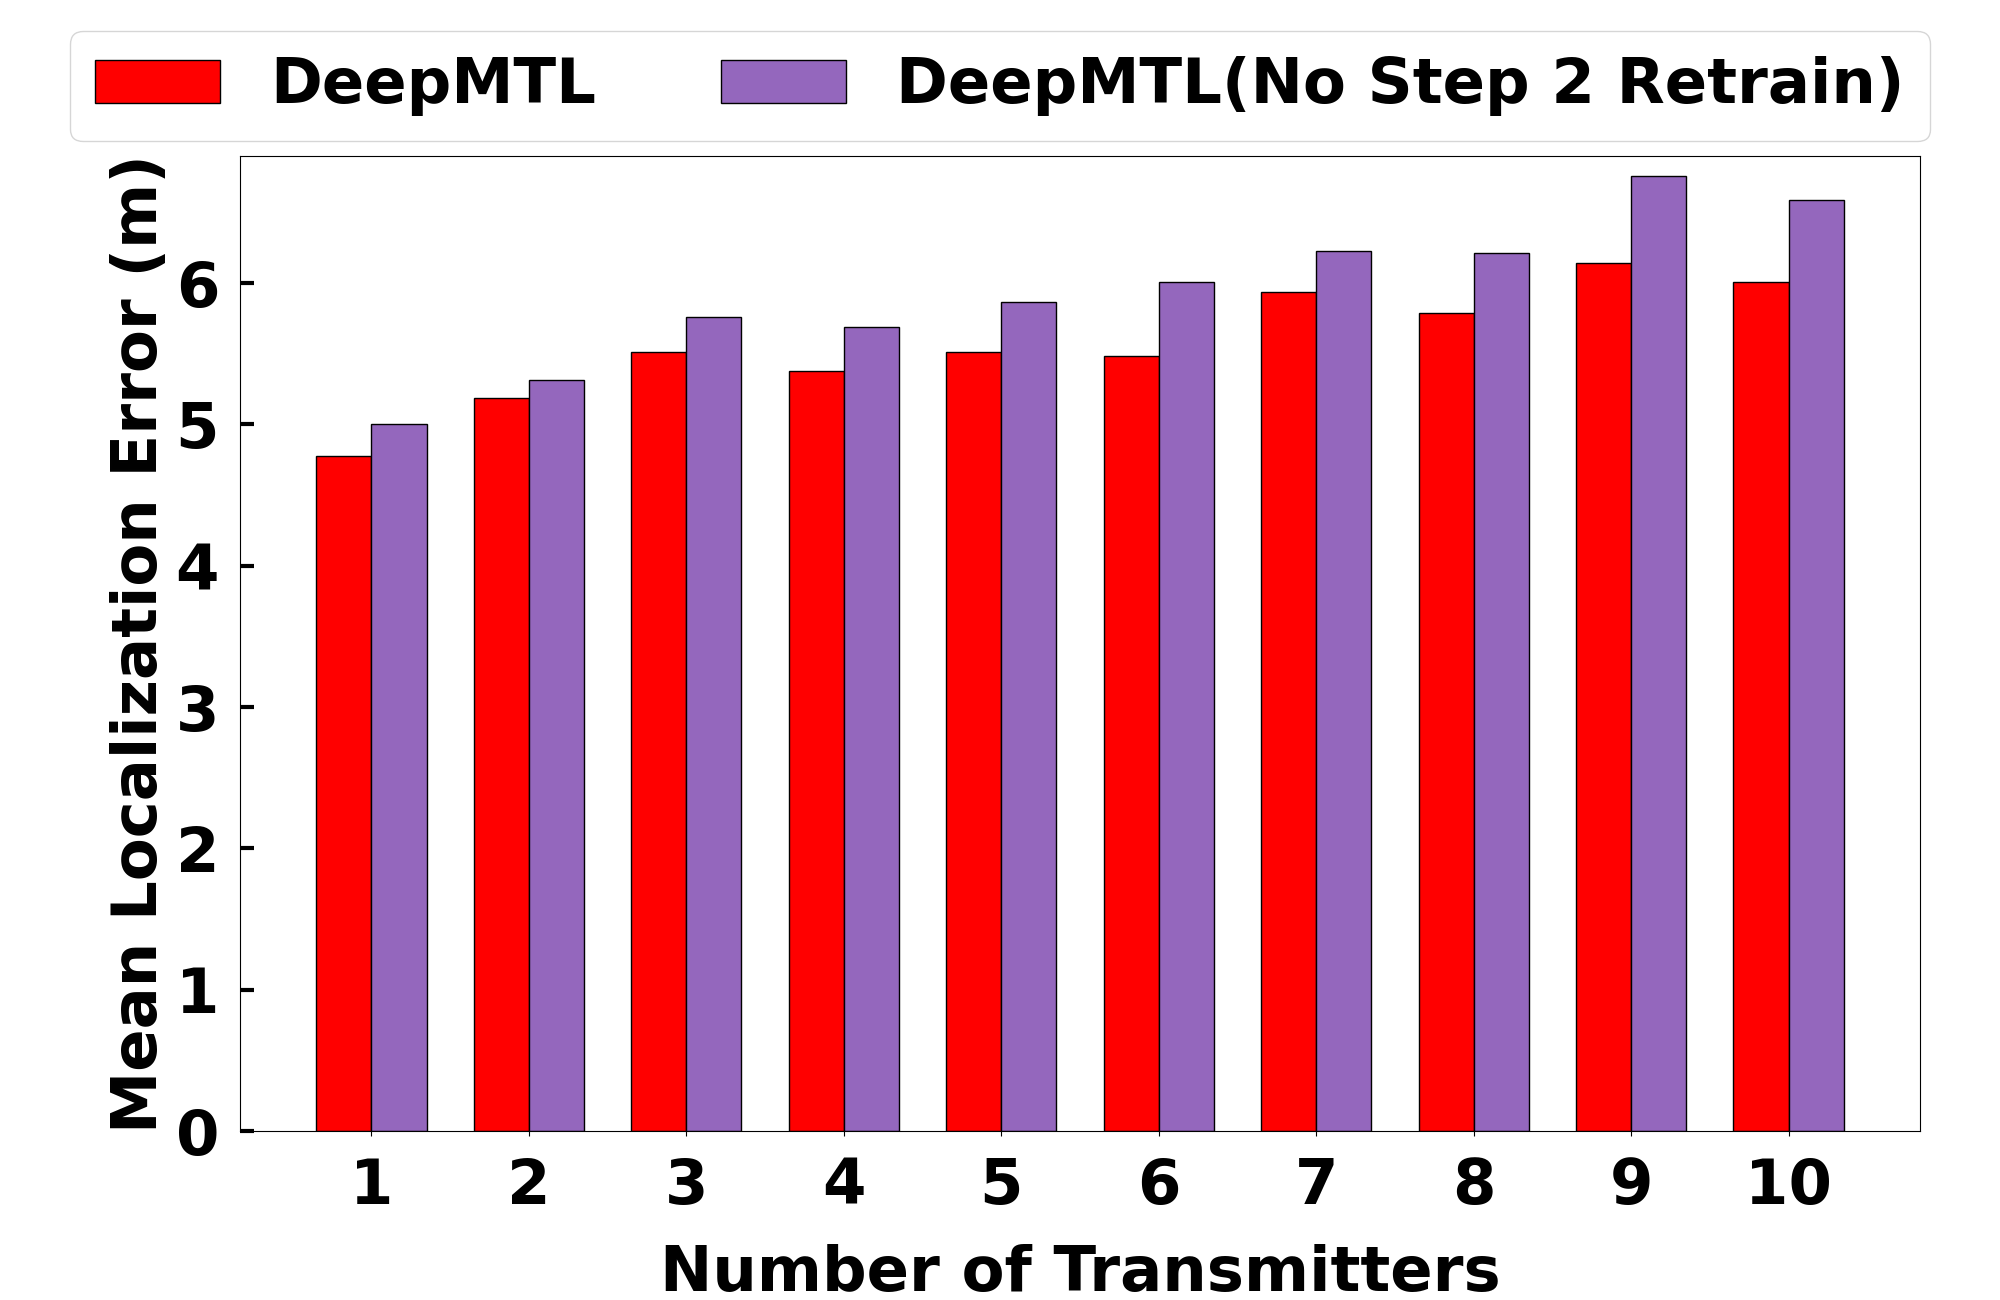
\includegraphics[width=\textwidth]{chapters/wowmom-pmc/figures/noretrain-splat-error-vary_numintru.png}
        \caption{First step trained in SPLAT! data, while second the step trained in log-distance data. Tested on the SPLAT! data.}
        \label{fig:notrain-splat}
    \end{subfigure}
    \caption{Localization error for varying number of transmitters when the first and second step of \our are trained on different training dataset.}
    \label{fig:notrain}
\end{figure*}

\begin{figure*}[t!]
    \centering
    \begin{subfigure}[t]{0.48\textwidth}
        \centering
        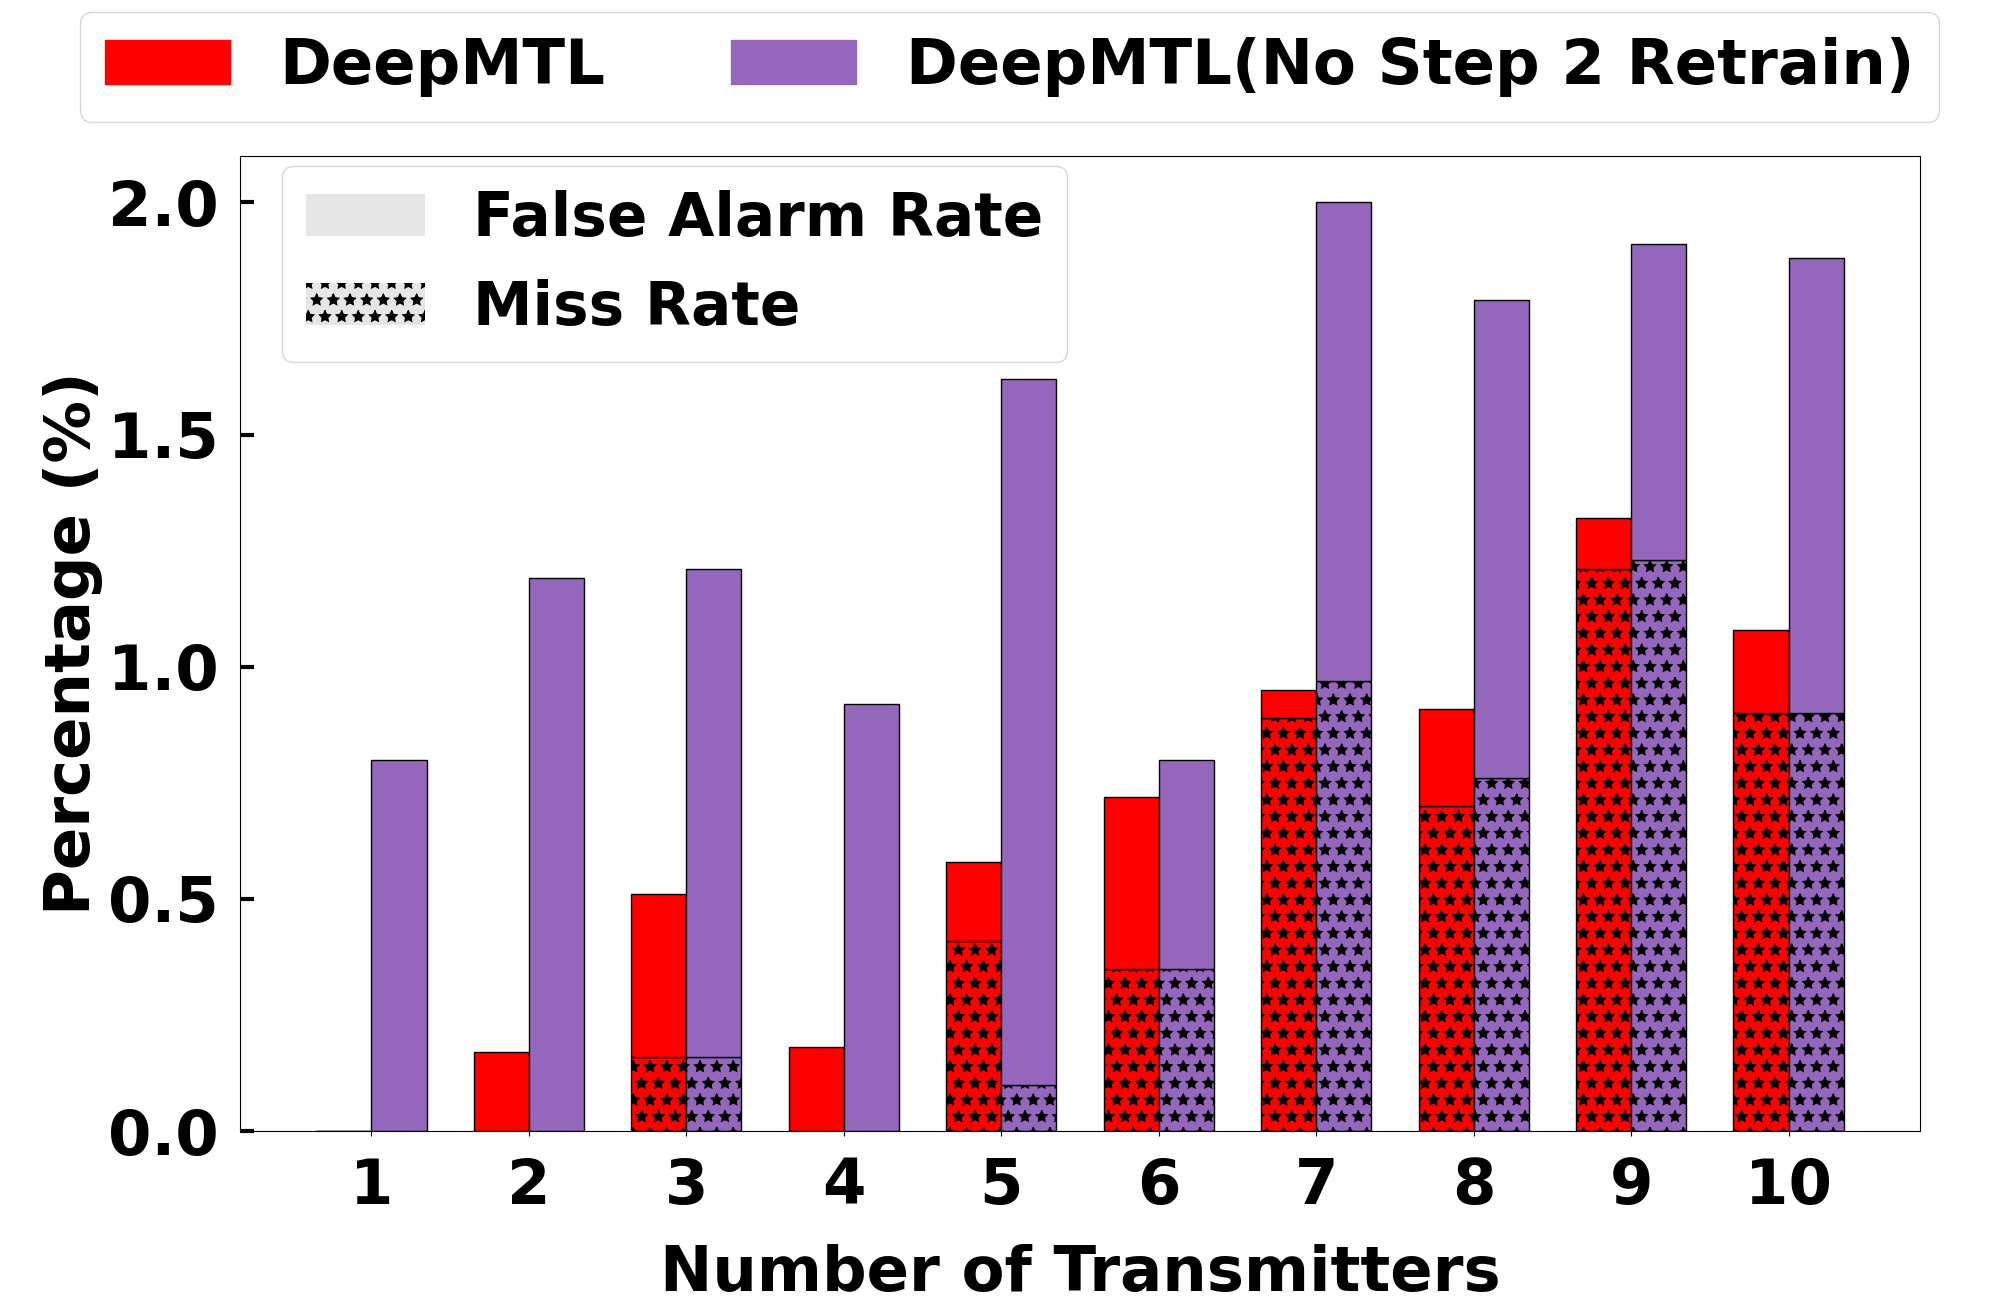
\includegraphics[width=\textwidth]{chapters/wowmom-pmc/figures/noretrain-logdistance-missfalse-vary_numintru.png}
        \caption{First step trained in log-distance data, while second step trained in SPLAT! data. Tested on the log-distance data.}
        \label{fig:notrain-logdist-missfalse}
    \end{subfigure}%
    ~ 
    \begin{subfigure}[t]{0.48\textwidth}
        \centering
        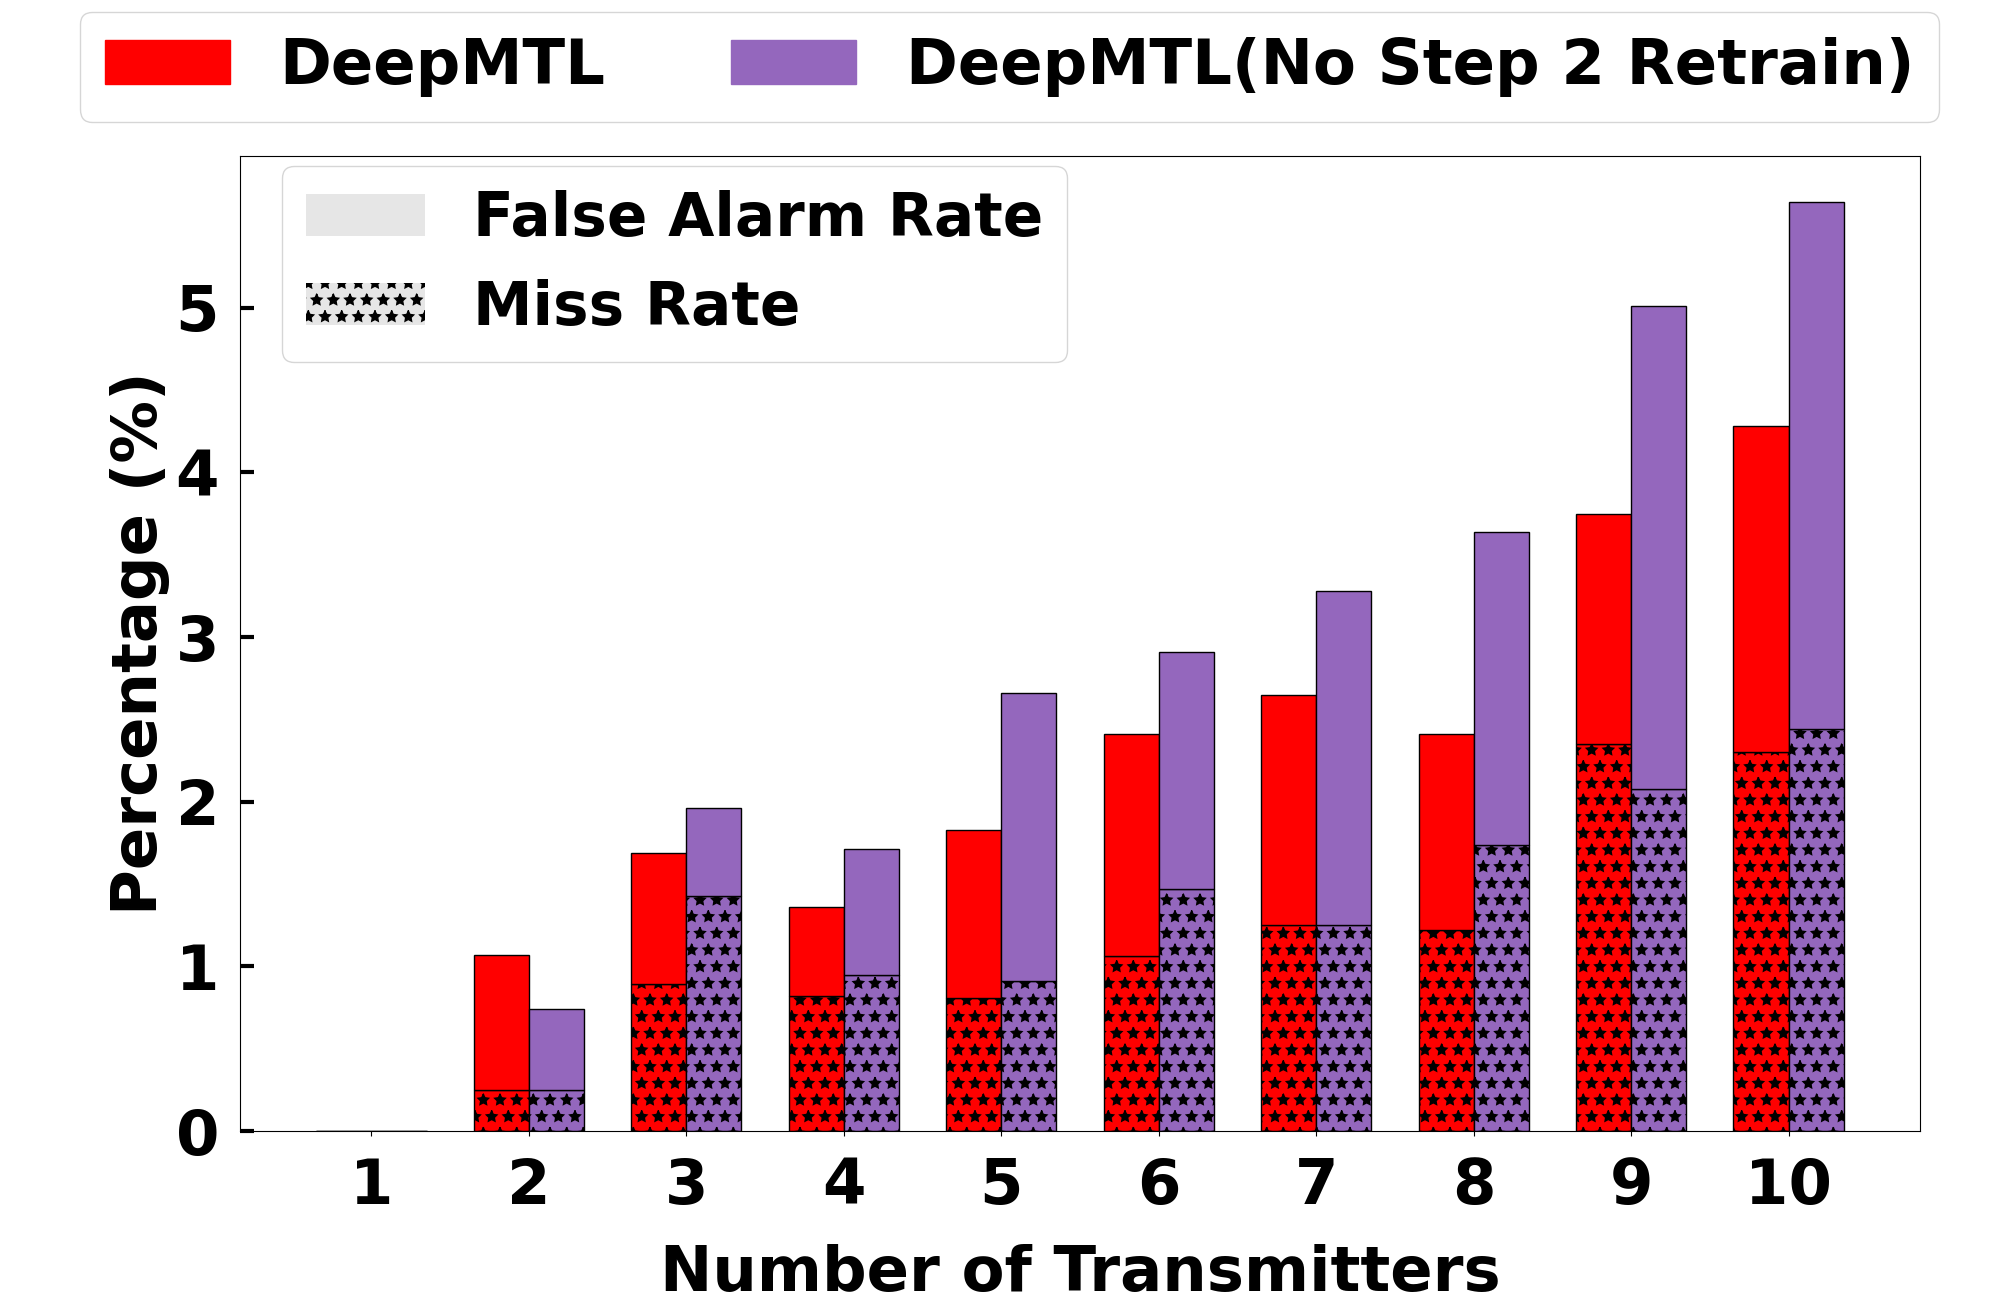
\includegraphics[width=\textwidth]{chapters/wowmom-pmc/figures/noretrain-splat-missfalse-vary_numintru.png}
        \caption{First step trained in SPLAT! data, while second step trained in log-distance! data. Tested on the SPLAT! data.}
        \label{fig:notrain-splat-missfalse}
    \end{subfigure}
    \caption{The miss rate and false alarm rate for varying number of transmitters when the first and second step of \our are trained on different training dataset.}
    \label{fig:notrain-missfalse}
\end{figure*}

We demonstrate transfer learning (generalizability) by showing that the second step in \our does not need to be retrained for different radio frequency propagation models and terrains.
In the previous experiments, the two steps of \our are both trained in the same setting, either log-distance or SPLAT!.
We do the following two combinations to show that the second step does not need to retrain:
\begin{enumerate}
    \item The first step is trained in the log-distance setting and the second step is trained in the SPLAT! setting. Tested on the log-distance data.
    \item The first step is trained in the SPLAT! setting and the second step is trained in the log-distance setting. Tested on the SPLAT! data.
\end{enumerate}
In both combinations, the second step \yolocust is trained on a different dataset compared to the first step \imgimg. 
Fig.~\ref{fig:notrain-logdist} shows that the localization error increases one-third in the first combination compared to the case where both the first and second steps are trained on log-distance dataset. 
Fig.~\ref{fig:notrain-splat} shows that the localization error increases only five percent in the second combination compared to the case where both the first and second steps are trained on SPLAT! dataset.
The miss rate and false alarm rate for both combinations also increase minimally, i.e. the summation of miss rate and false alarm rate only increases around 1\% in absolute value. See Fig.~\ref{fig:notrain-missfalse}.
This implies that the second step of \our, \yolocust, is general and does not need to retrain for different radio frequency propagation models and terrains.
This is because the first step \imgimg is translating sensor readings images from different geographical areas to the same Gaussian peaks.
The first step \imgimg still needs to be retrained for different situations to translate the sensor readings to the peaks.


\subsection{Localize Intruders in the Presence of Authorized Users}
\label{subsec:authorzedeval}

The previous experiment setting is based on the assumption that all transmitters we are localizing are intruders.
Different than the previous setting, here, we put five authorized users and they are spread out in the field, so those five will not interfere with each other.
This is the more general version of the \mtl problem, where there are some authorized users in the background.
Fig.~\ref{fig:authorized_error} shows the localization error of two approaches localizing intruders in the presence of five authorized users with a varying number of intruders.
It is observed that the first approach, localize then remove authorized users, has a ten to twenty percent smaller localization error compared to the second approach, subtract authorized user power then localize.
This is due to the inaccuracy of power subtraction from the \subtract.
Fig.~\ref{fig:authorized_missfalse} shows the miss and false alarm of two approaches localizing intruders in the presence of five authorized users with a varying number of intruders.
It is observed that the second approach, subtract authorized TX power then localize, is having a high false alarm when the number of intruders is three or less.
So for \subtract, subtracting the power of five background authorized users from six transmitters (five out of six transmitters are authorized users, one intruder) is relatively more difficult than subtracting the power of five authorized users from nine users (five out of nine transmitters are authorized users, four intruders). 
Also statistically, getting one false alarm when there are one intruder and five authorized users is 100\% false alarm rate, while getting one false alarm when there are two intruders and five authorized users is only 50\% false alarm rate (the denominator is the number of intruders).
Thus, the false alarm rate for one and two number of intruders looks to differ a lot, but in reality, the false alarm cases do not differ a lot).
When the number of intruders is three or four, the two approaches are comparable. But when the number of intruders is larger than four, the second approach is having a lower miss and false alarm rate.
In summary, the two approaches both have their strengths.
The main advantage for the second approach is that the sum of miss rate and false alarm rate is lower when the number of intruders is large.

\begin{figure}[t]
    \centering
    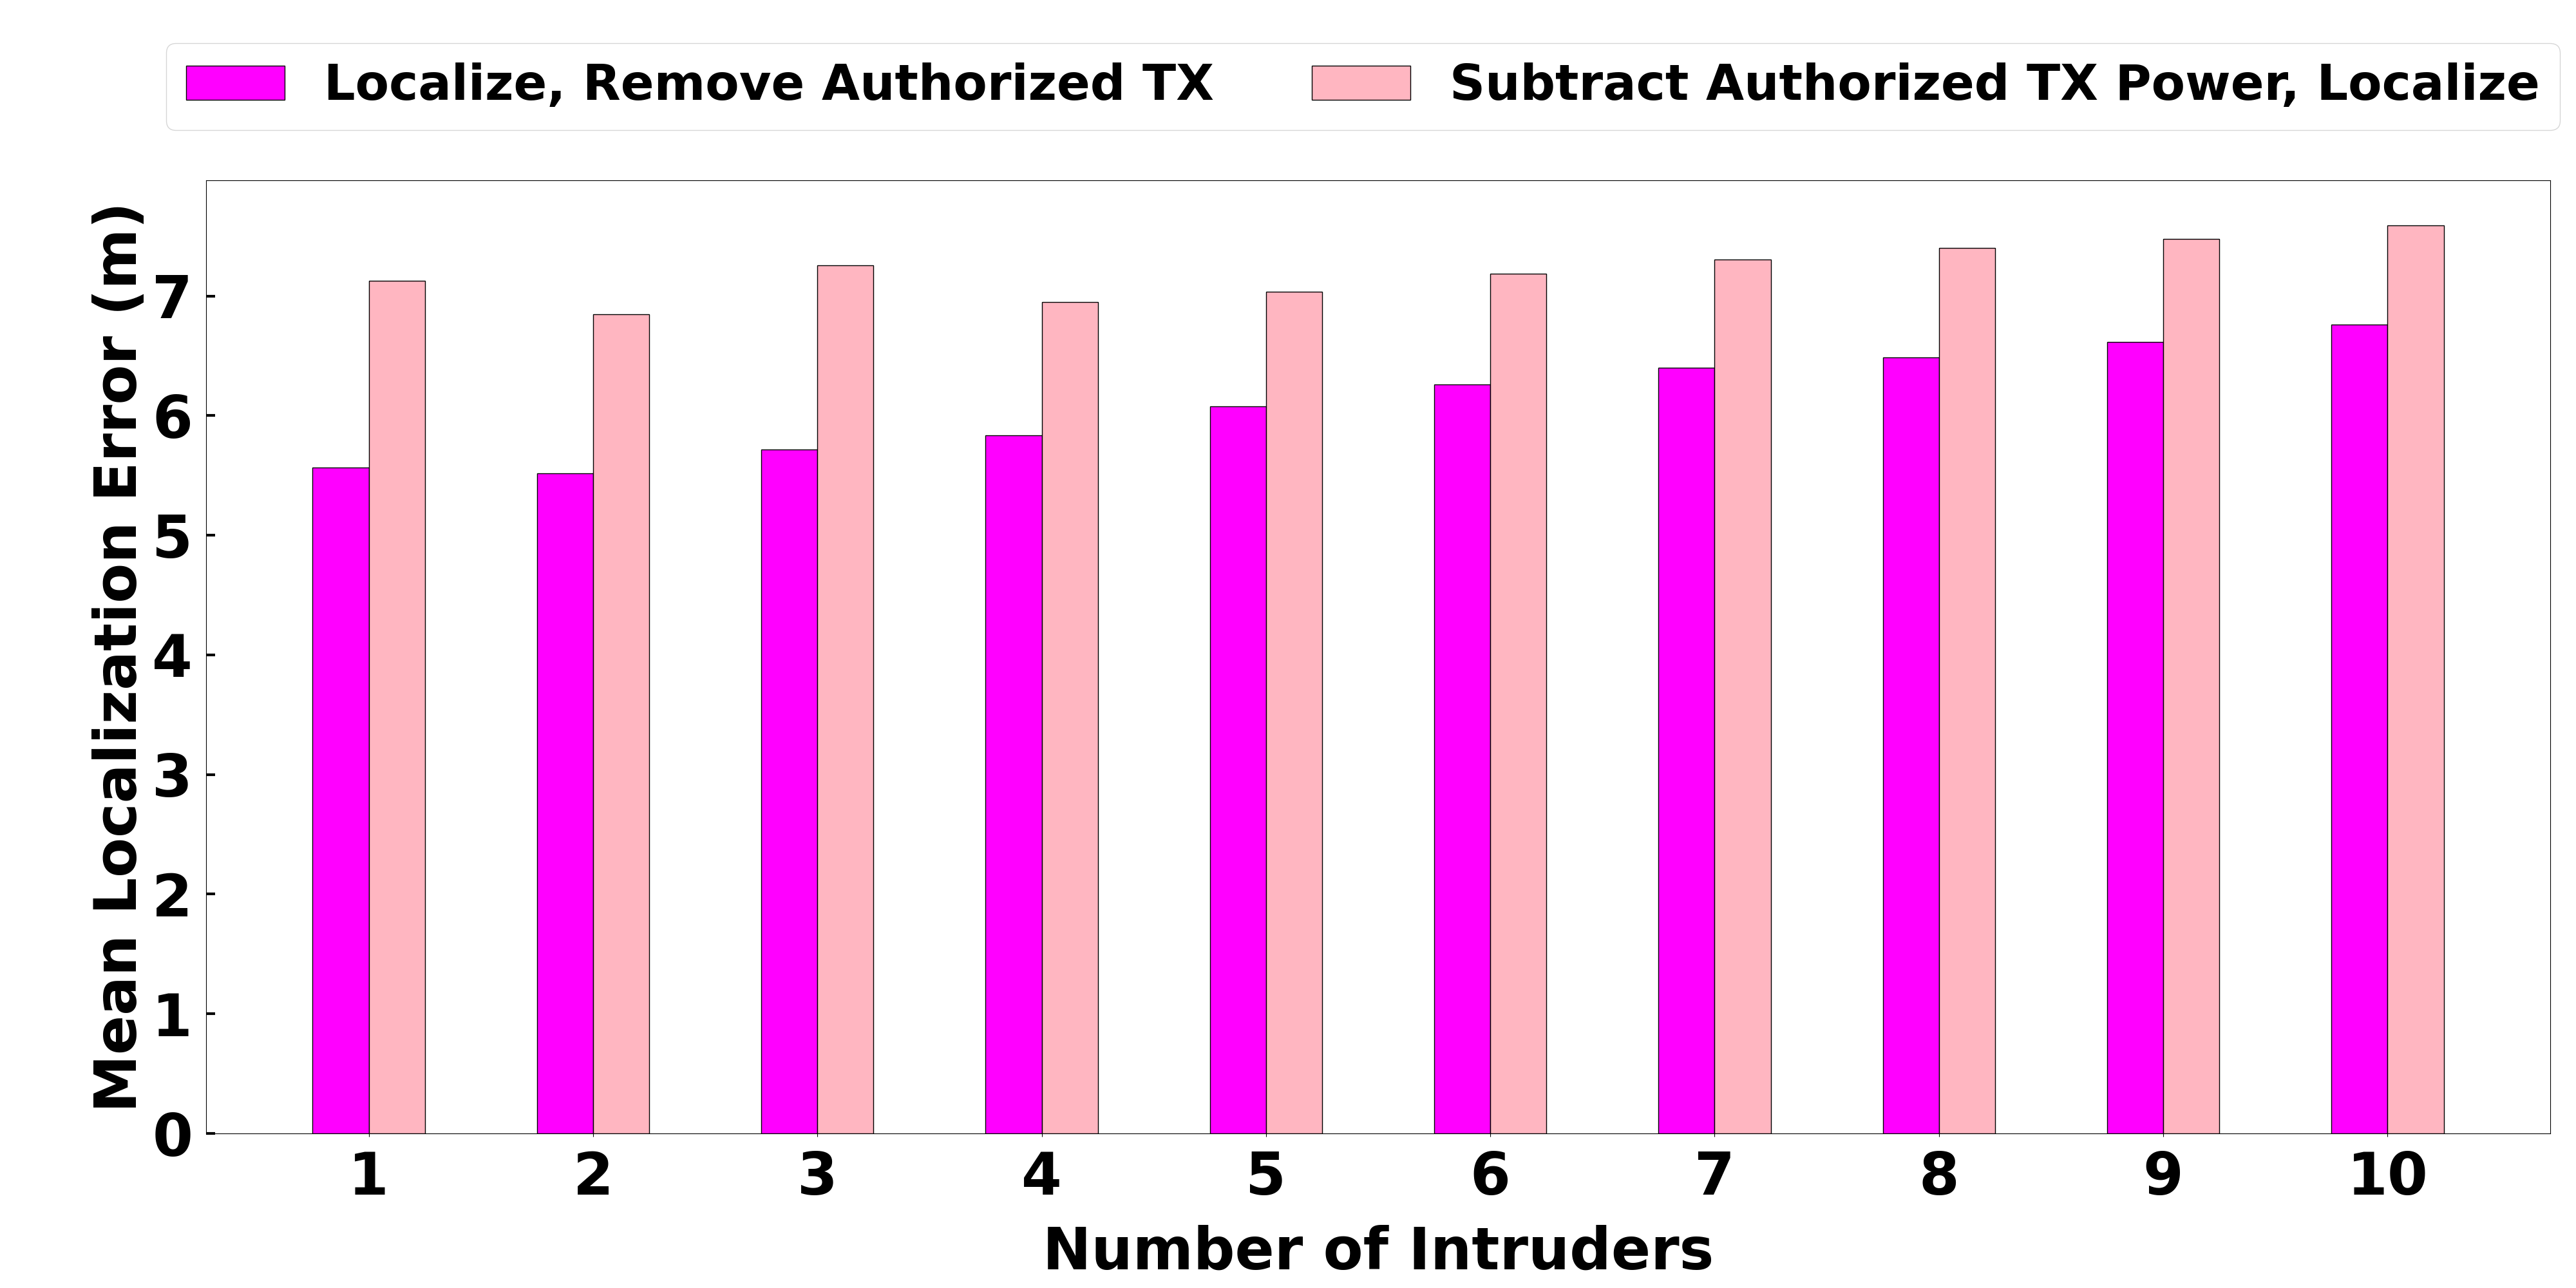
\includegraphics[width=0.75\textwidth]{chapters/wowmom-pmc/figures/splat-error-authorized-varyintru.png}
    \caption{The localization error of two approaches in the presence of five authorized users with varying number of intruders.}
    \label{fig:authorized_error}
\end{figure}

\begin{figure}[t]
    \centering
    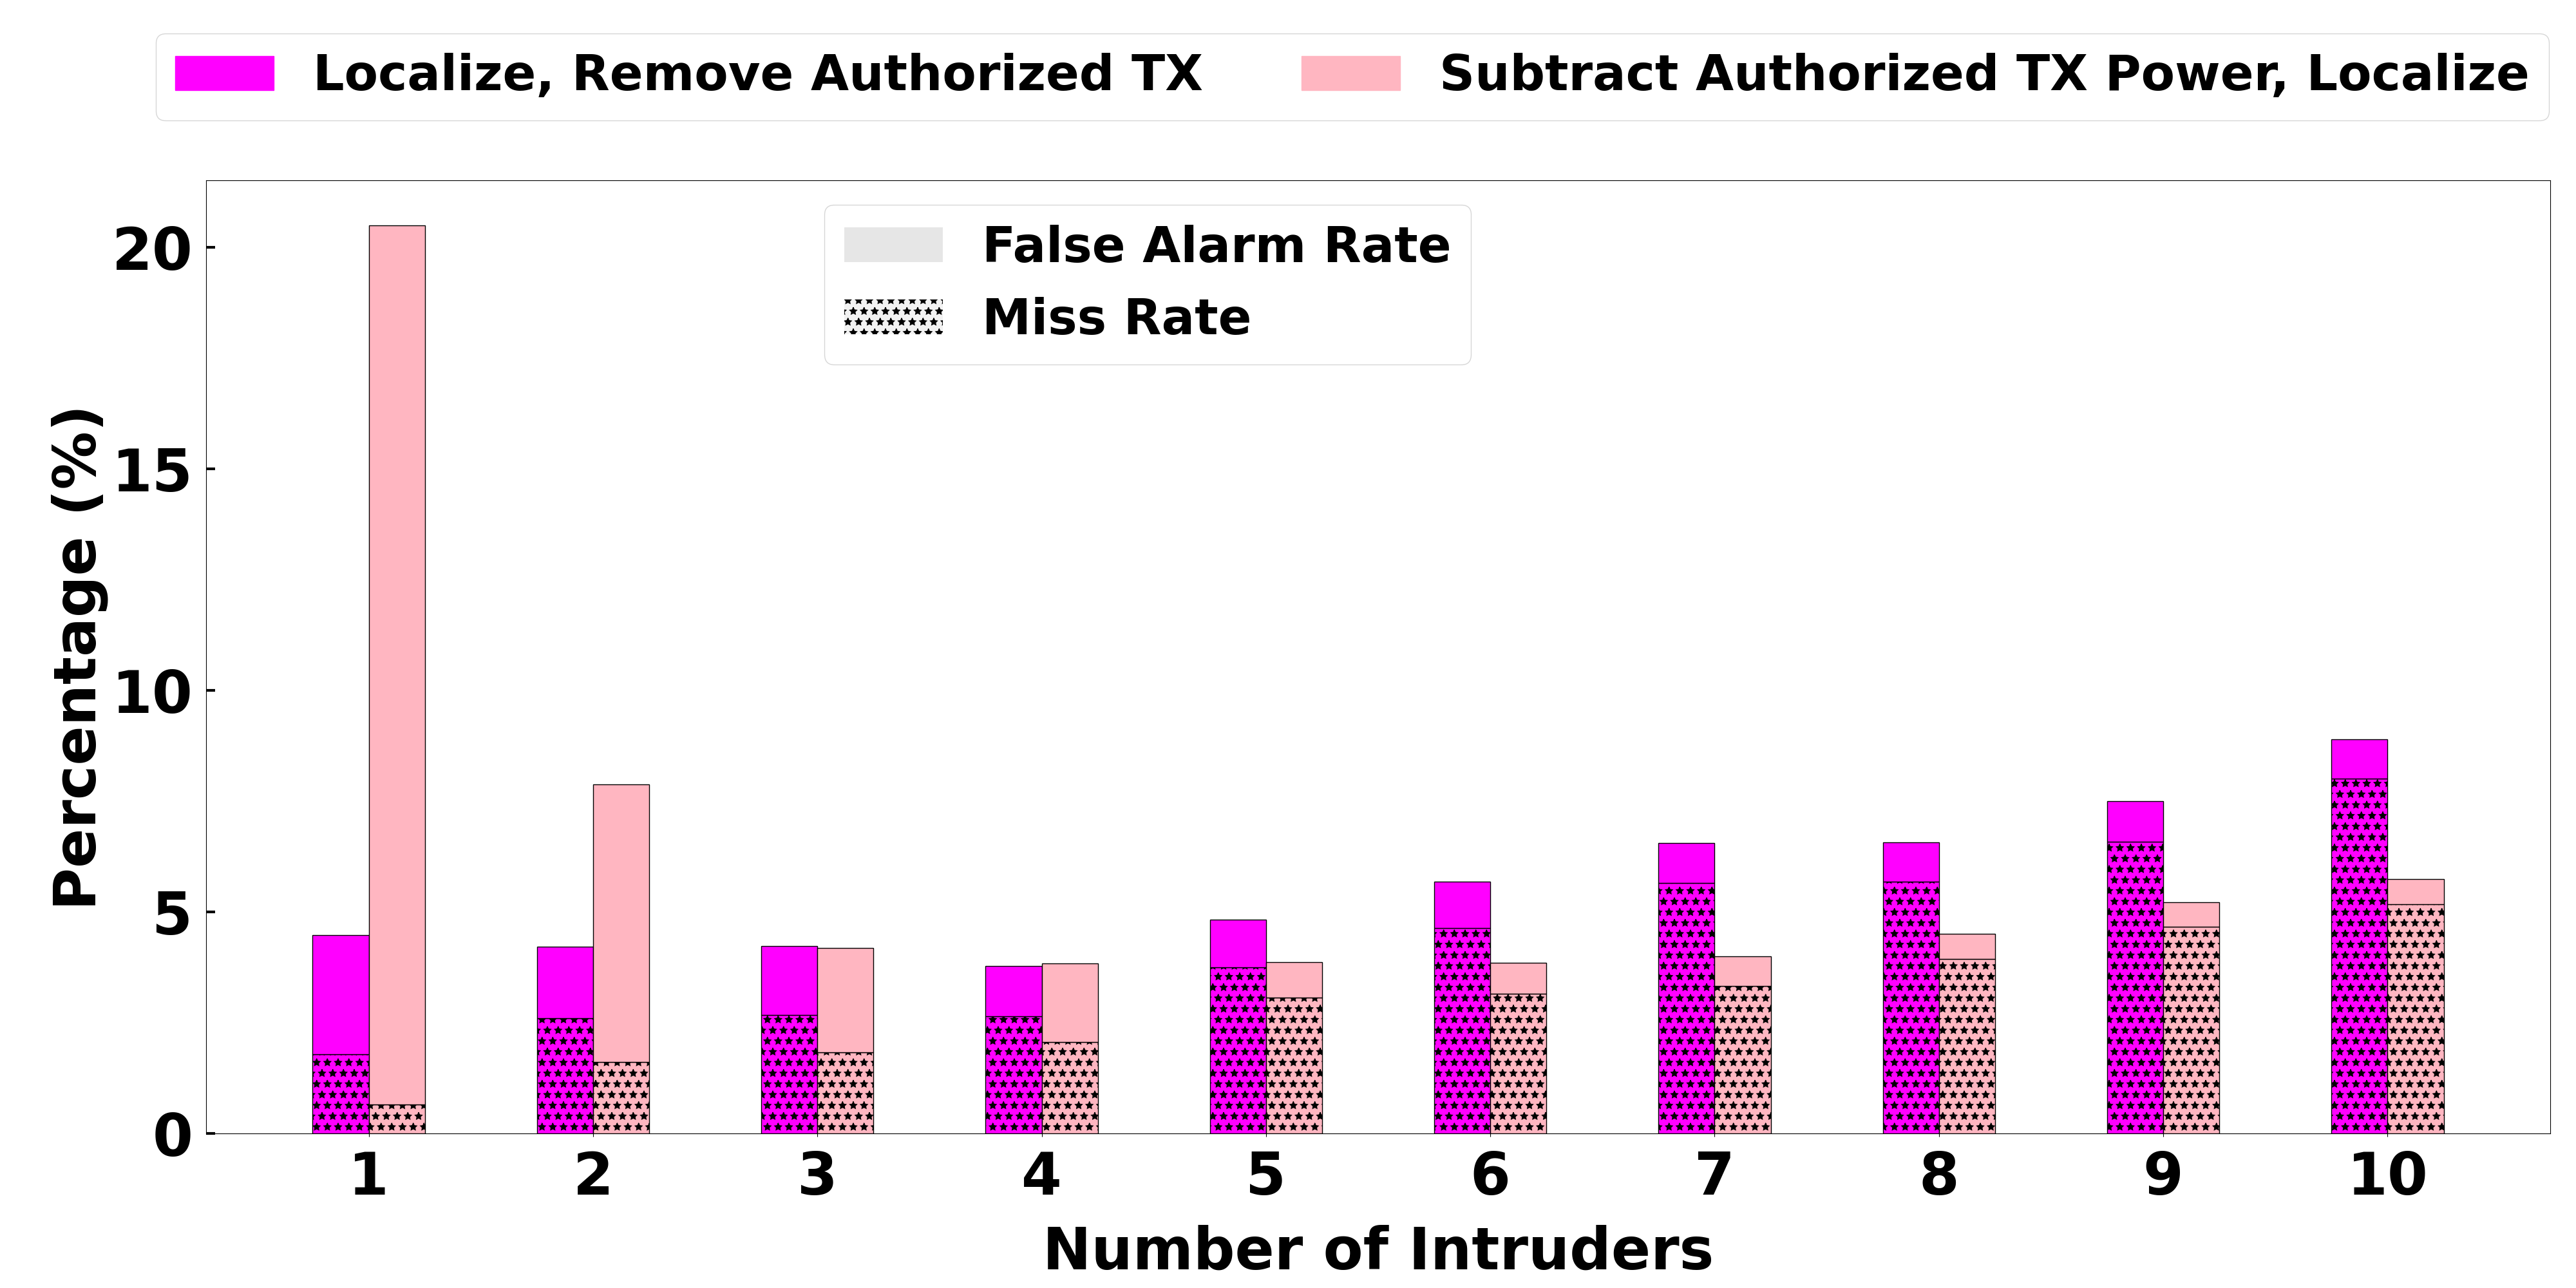
\includegraphics[width=0.75\textwidth]{chapters/wowmom-pmc/figures/splat-missfalse-authorized-varyintru.png}
    \caption{The miss and false alarm of two localization approaches in the presence of 5 authorized users with varying number of intruders.}
    \label{fig:authorized_missfalse}
\end{figure}




\subsection{Power Estimation Evaluation}
\label{subsec:powereval}
In this subsection, we evaluate the transmitter power estimation performance.
In all experiments, the power range is 5 dB.
The power error is presented in absolute value.
A power error of 0.5 dB implies a relative power error of 10\%.
First, we compare the single transmitter power estimation between \map and \power, and then compare the multiple transmitter power estimation between \map, \power with error correction, and \power with error correction.

\begin{figure}
    \centering
    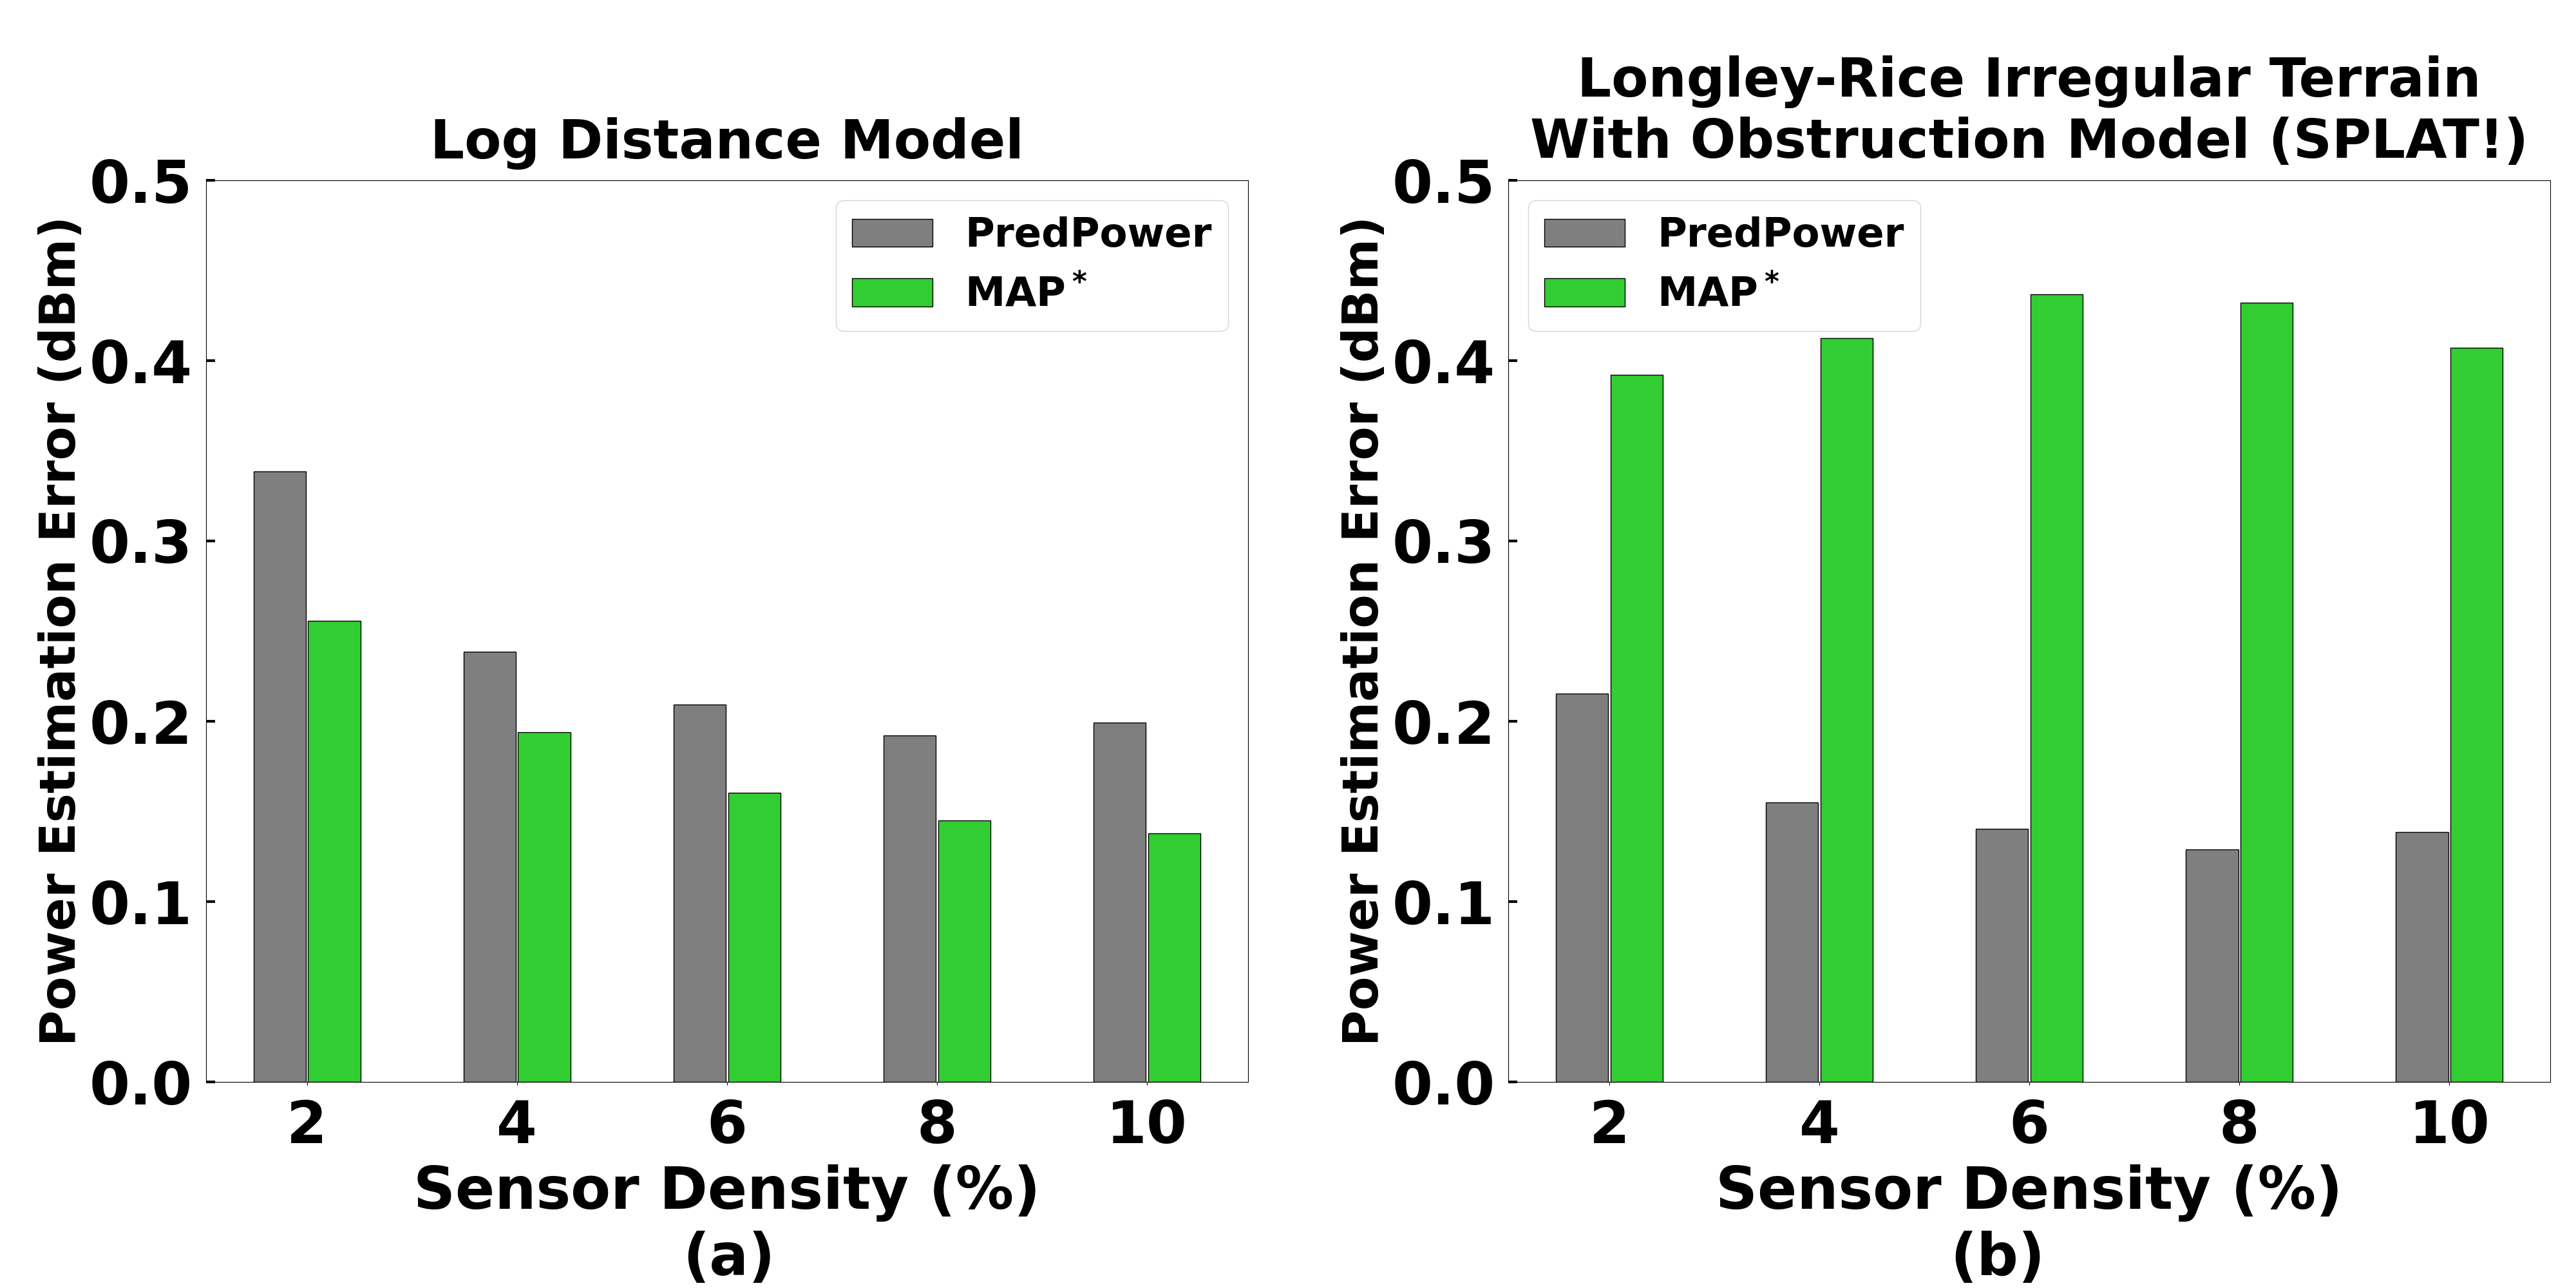
\includegraphics[width=0.75\textwidth]{chapters/wowmom-pmc/figures/powererror_varysensor.png}
    \caption{The single transmitter power estimation error of \power and \map in two propagation models, (a) Log-distance model and (b) Longley--Rice Irregular Terrain with Obstruction Model (SPLAT!), for varying sensor densities.}
    \label{fig:singleTXpower}
\end{figure}

Figure~\ref{fig:singleTXpower}(a) shows the performance of single transmitter power estimation in the log-distance propagation model scenario with varying sensor density.
In this case, \map has a 10 to 20 percent smaller power estimation error.
Figure~\ref{fig:singleTXpower}(b) shows the performance of single transmitter power estimation in the SPLAT! model with varying sensor density.
In this case, \power is significantly lower in power error.
So in average, \power outperforms \map in single transmitter power estimation.
We can also conclude that for \power, a higher sensor density will decrease the power estimation error. \
While a 2\% of sensor density will lead to a higher error, a sensor density of 6\% is enough to give relatively good results.

For multiple transmitter power estimation, we compare three methods in two propagation models and show that \power with error correction has the best performance among the three methods.
\power without error correction is expected to perform the worst and it suggests that the post-processing error correction stage for \power is important and works well.
%%%
\begin{figure}[t]
    \centering
    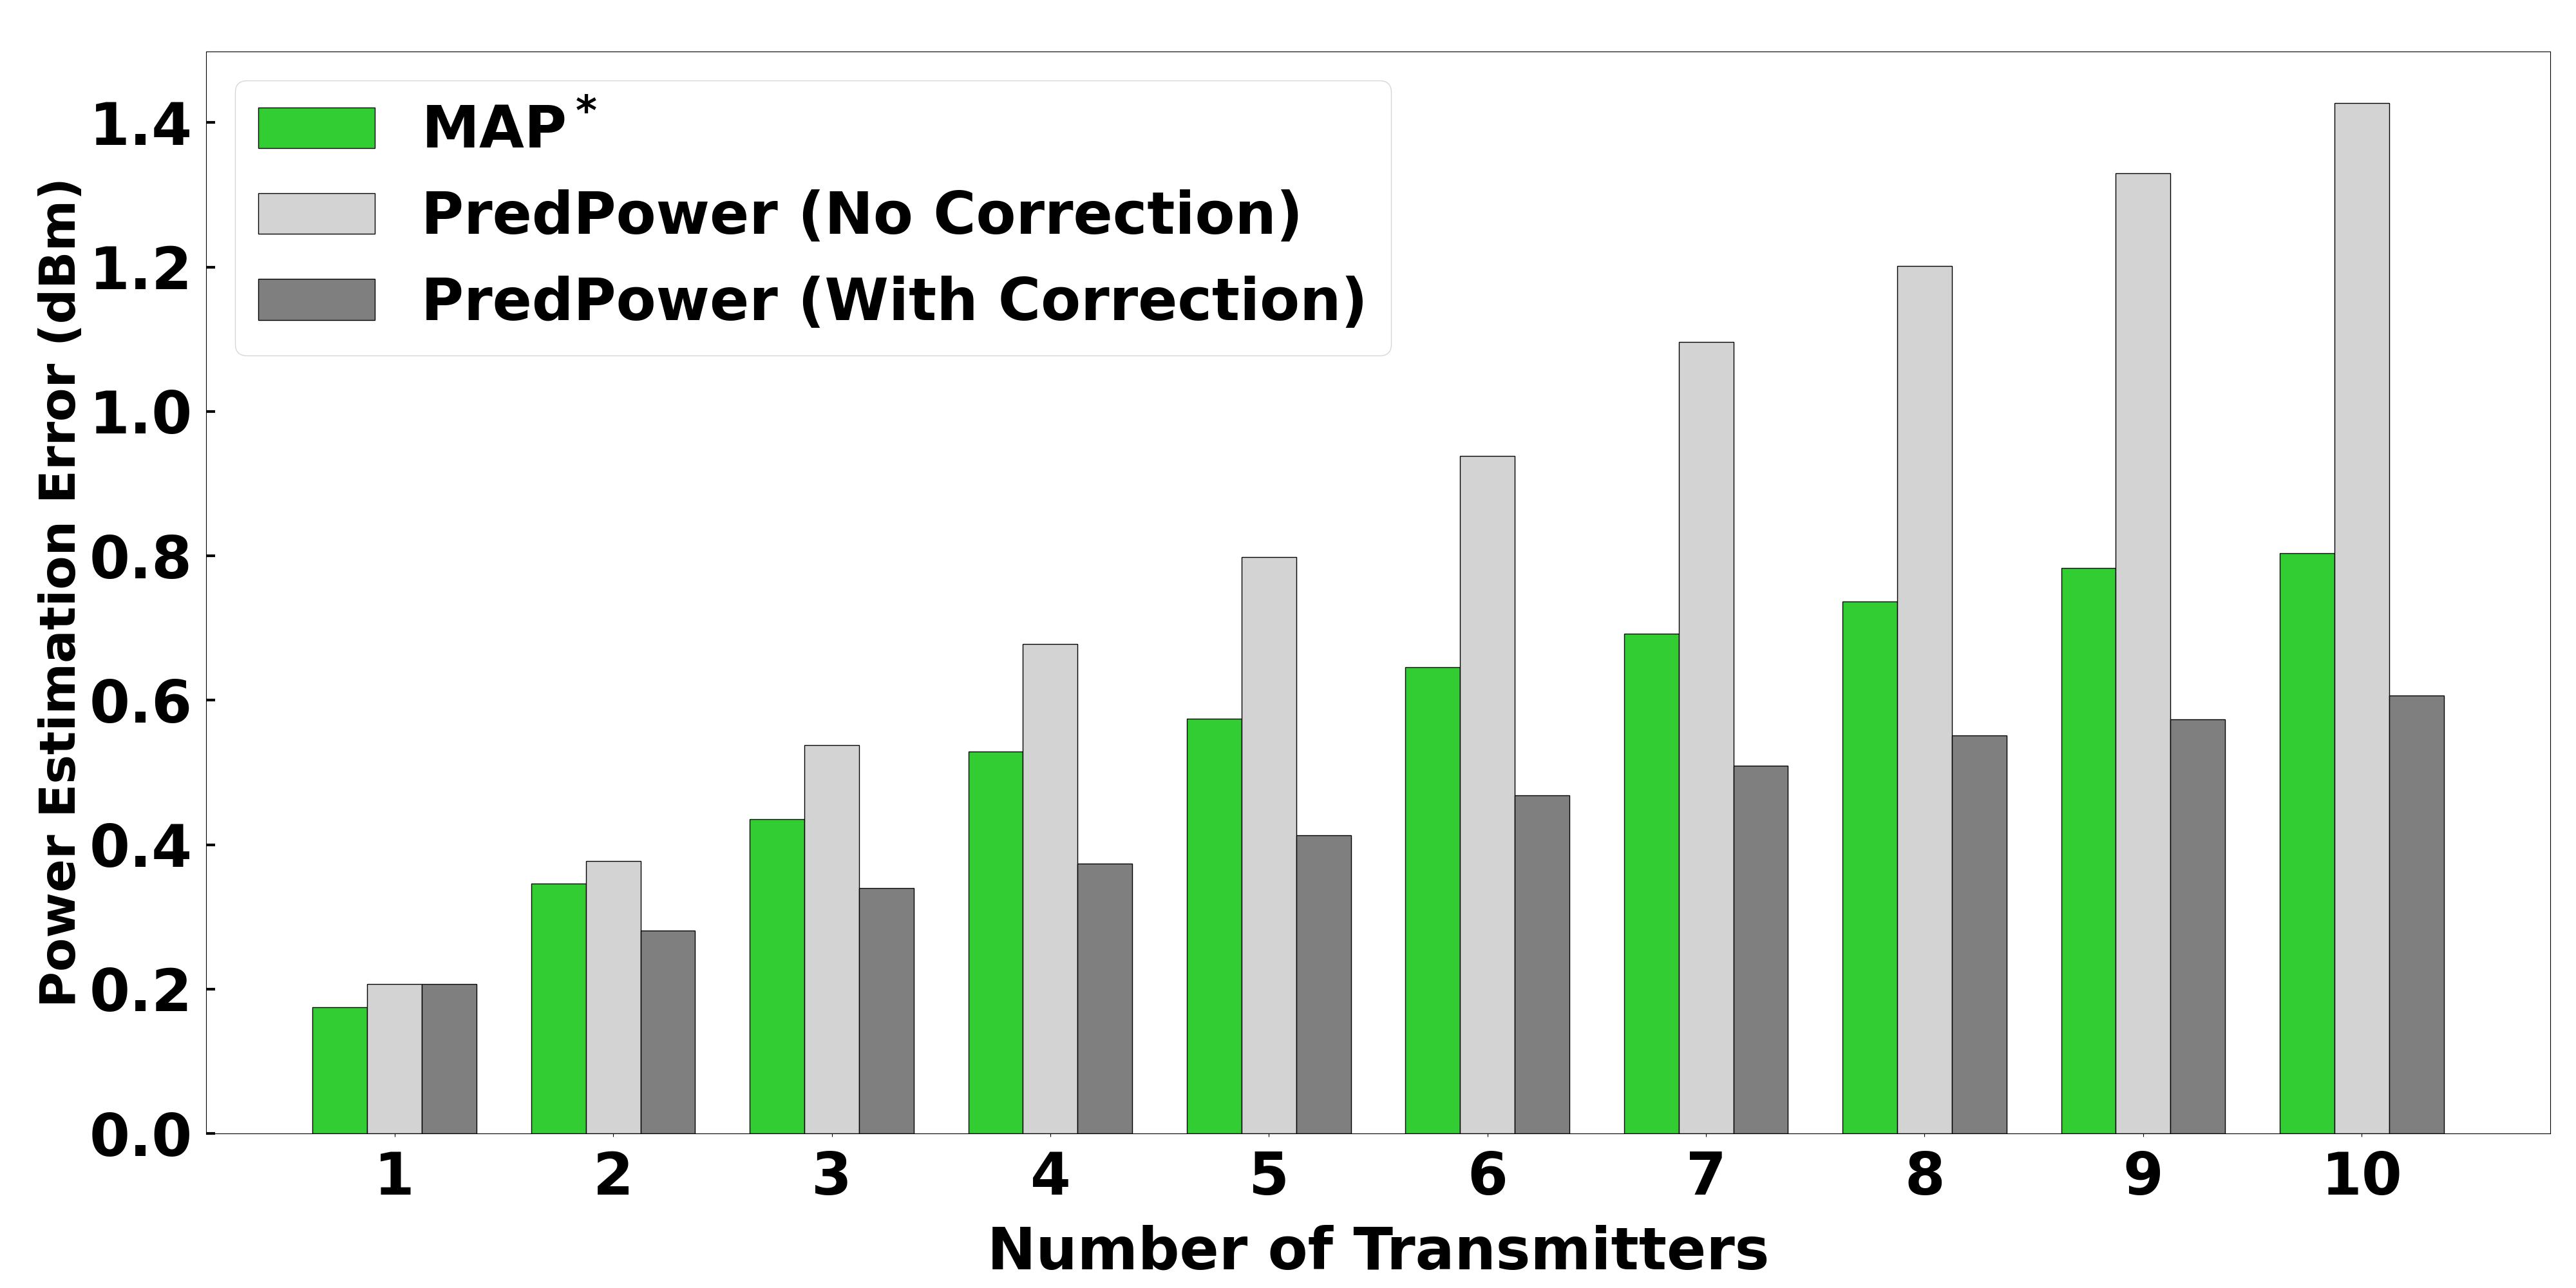
\includegraphics[width=0.75\textwidth]{chapters/wowmom-pmc/figures/logdist-powererror_varyintru.png}
    \caption{The transmitter power estimation error of \map, \power with and without correction in Log-distance model for varying number of intruders}
    \label{fig:logdistance-multiTXpower}
\end{figure}
\begin{figure}[t]
    \centering
    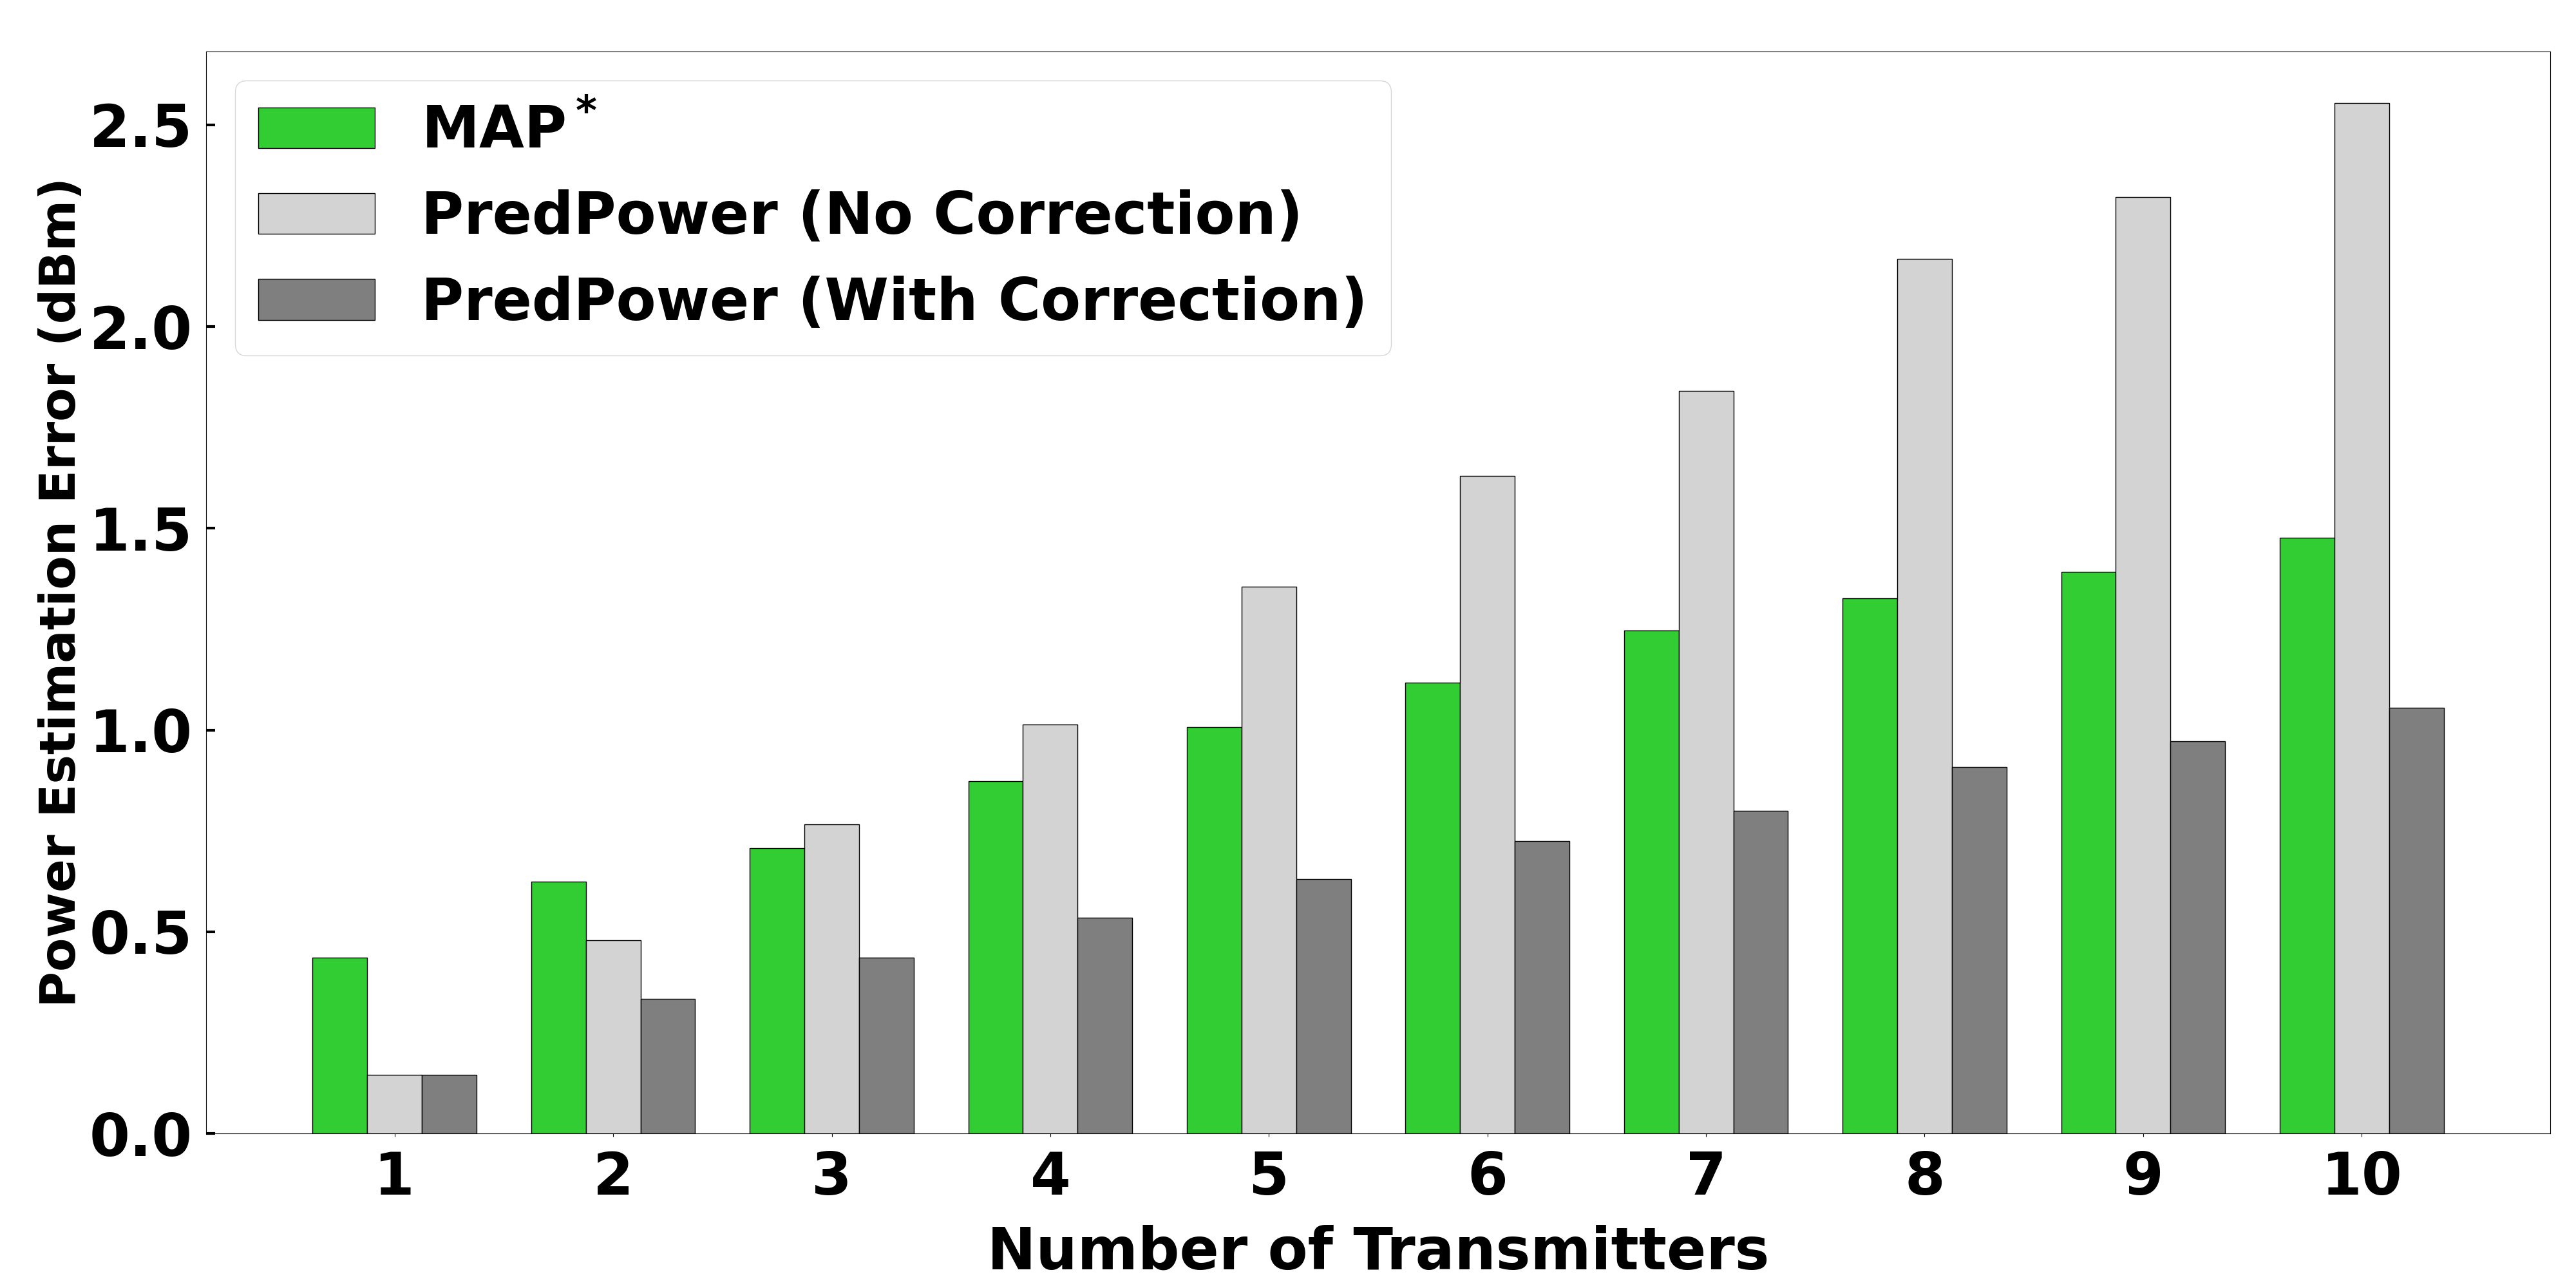
\includegraphics[width=0.75\textwidth]{chapters/wowmom-pmc/figures/splat-powererror_varyintru.png}
    \vspace{-0.1in}
    \caption{The transmitter power estimation error of \map,  \power with and without correction in Longley--Rice Irregular Terrain with Obstruction Model (SPLAT!) for varying number of intruders.}
    \label{fig:splat-multiTXpower}
\end{figure}
%%%
Figure~\ref{fig:logdistance-multiTXpower} shows the power estimation error of three methods with a varying number of transmitters while the sensor density is 6\%.
In this figure, \map is the best only when the number of transmitters is one (which is consistent with Fig~\ref{fig:singleTXpower}(a)).
Also the number of transmitters is one is the only case when \power with correction and without correction has the same performance.
This is also expected because there is no need to error correction when there is only one transmitter in the area.
In all other cases, we see that \power with error correction is the best, \power without error correction  is the worst, and \map is in the middle.
In Figure~\ref{fig:splat-multiTXpower}, which shows experiment results running in the SPLAT! propagation model, we see a similar pattern compared to Figure~\ref{fig:logdistance-multiTXpower}.
The difference is that \power with error correction is always the best and the power error is larger than the log-distance model scenario.
For example in Figure~\ref{fig:logdistance-multiTXpower}, the power estimation error for \power with error correction goes up to 0.6 dB, where as in Figure~\ref{fig:splat-multiTXpower}, the error goes up to 1 dB.







\subsection{Evaluation over Testbed Data}
\label{subsec:ipsn}
In this subsection, we show that our \our performs well in real-world collected data.
For this, we repurpose our testbed data from~\cite{ipsn20-mtl} as described below. We start with describing our testbed data from~\cite{ipsn20-mtl}.

\para{Testbed Data.}
In \cite{ipsn20-mtl}, we conducted a testbed in an outdoor parking area of $32m\times 32m$ large.\footnote{Dataset publicly available at: \url{https://github.com/Wings-Lab/IPSN-2020-data}}
Each grid cell has a size of $3.2m \times 3.2m$, with the grid size being $10\times 10$.
We place a total of 18 sensors on the ground.
The sensors consist of Odroid-C2 (a single-board computer) connected to an RTL-SDR dongle and the RTL-SDR connects to dipole antennas.
The transmitters are USRP or HackRF connecting to a laptop.
We collect raw Inphase-Quadrature (I/Q) samples from the RTL-SDR at the 915 MHz ISM band.
We perform FFT on the I/Q samples with a bin size of 256 samples to get the signal power values, and then utilize the mean and standard deviation of the power at frequency 915 MHz reported from each of the sensors.

\para{Transforming the Data from $10 \times 10$ to $100 \times 100$ Grid.}
Note that \our's input requires a $100\times 100$ input, while the above data is over a
 $10\times 10$ grid. Also, the sensor density in the above data is 18\%, while we desire a sensor
 density of around 4-6\% to have a fair comparison with our simulation based evaluations in previous subsections. To achieve these objectives, we transform the above $10 \times 10$ data to a $100 \times 100$ grid data in two steps as follows.
% So, the second goal is to transform the sensor density to fall in the middle of the sensor density ranged used in the simulated based evaluations, which is 1\% to 10\%, for a fair comparison.
% Duplication and increasing granularity are two methods we use to transform the testbed data.
% If we only duplicate the $10\times10$ grid a hundred times to $100\times100$, then the sensor density will remain at 18\%, which is too high.
% If we only increase the granularity to $100\times100$, then the sensor density will drop to 0.18\%, which is too low.
%Thus, we use a combination of the two methods to satisfy the two goals, as described in the following two steps.}
\begin{enumerate}
    \item Increase the data granularity from $10 \times 10$ to $20\times 20$, by dividing each cell into $2 \times 2$ cells; we randomly pick one of these four smaller cells to represent the original cell (i.e., to place the sensor if it existed in the original cell). See the red-bordered boxes in Fig.~\ref{fig:testbed}(a)-(b). We refer to the full $20 \times 20$ grid as a \emph{tile}.
    \item Now, we duplicate the $20\times20$ tile $25$ times using a $5 \times 5$ pattern to generate a  $100 \times 100$ grid. See Fig.~\ref{fig:testbed}(b)-(c).
\end{enumerate}
The above steps effectively increase the area from the original $32m\times32m$ to $160m\times160m$. 
Note that the first step above only splits each original cell into four smaller cells without increasing the whole area size.
The $100\times100$ grid will have a sensor density of 4.5\% and each grid cell represents an area of $1.6m\times1.6m$.



%\blue{Note that the grid size is the only relevance during the grid transformation, not the area that the grid represents.
%However, after transforming the $10\times10$ grid into a $100\times100$ grid, the new grid will represent a different area.
% A tile's area is $32m\times32m$ large, which is the same as the original $10\times10$ grid. 
% But after duplicating to 25 tiles, the new $100\times100$ grid will represents a larger area of $160m\times160m$.
% The new $100\times100$ size grid will have a sensor density of 4.5\% and each grid cell represents an area of $1.6m\times1.6m$.}

We note that the second duplication step can introduce inaccurate sensor readings at the tile's ``edges", due to 
any transmitters from adjoining tiles. To circumvent this issue, we place {\em transmitters} only within the internal
$10 \times 10$ cells of each $20 \times 20$ tile (i.e., avoid placing a transmitter on the five-cell edge of each tile). This
yields a total of 2500 potential positions to place a transmitter in the final $100 \times 100$ grid. 
With the above setting, we generate training and testing datasets consisting of 25,000 and 12,500 samples respectively.
% The transmitters, however, cannot be placed at every possible location.
% For every tile, the transmitters will not be located at the edges.
% Because if so, there will be no RSSI observation data for the sensors at the edge of neighbor tiles.
% The edge's width equals to five cells. 
% When a transmitter is inside a tile, only the sensors inside the same tile will receive some signals from that transmitter (the sensors at the neighbor tile's edge will be ignored).
% \eat{Also, the increase of granularity (step 1) leads to only every one in four cells are legit sensor locations, these legit sensor locations will also be the legit transmitter locations.
% So for each tile, the legit cell locations for a transmitter is $(20-5\times2)^2 = 100$.
% Given 25 tiles, the total legit cell locations for a placing a transmitter is $100\times25=2500$.
% For multiple transmitters, they are randomly picked from these 2500 grid cells (a transmitter's location is still continuous inside the grid cell).
% A sensor receives an aggregated signal power from multiple transmitters.
%Thus, we can generate a $100\times100$ size input data that can be used by \our from a much smaller data of size $10\times10$ with a combination of granularity increase and duplication.}

\begin{figure}[t]
    \centering
    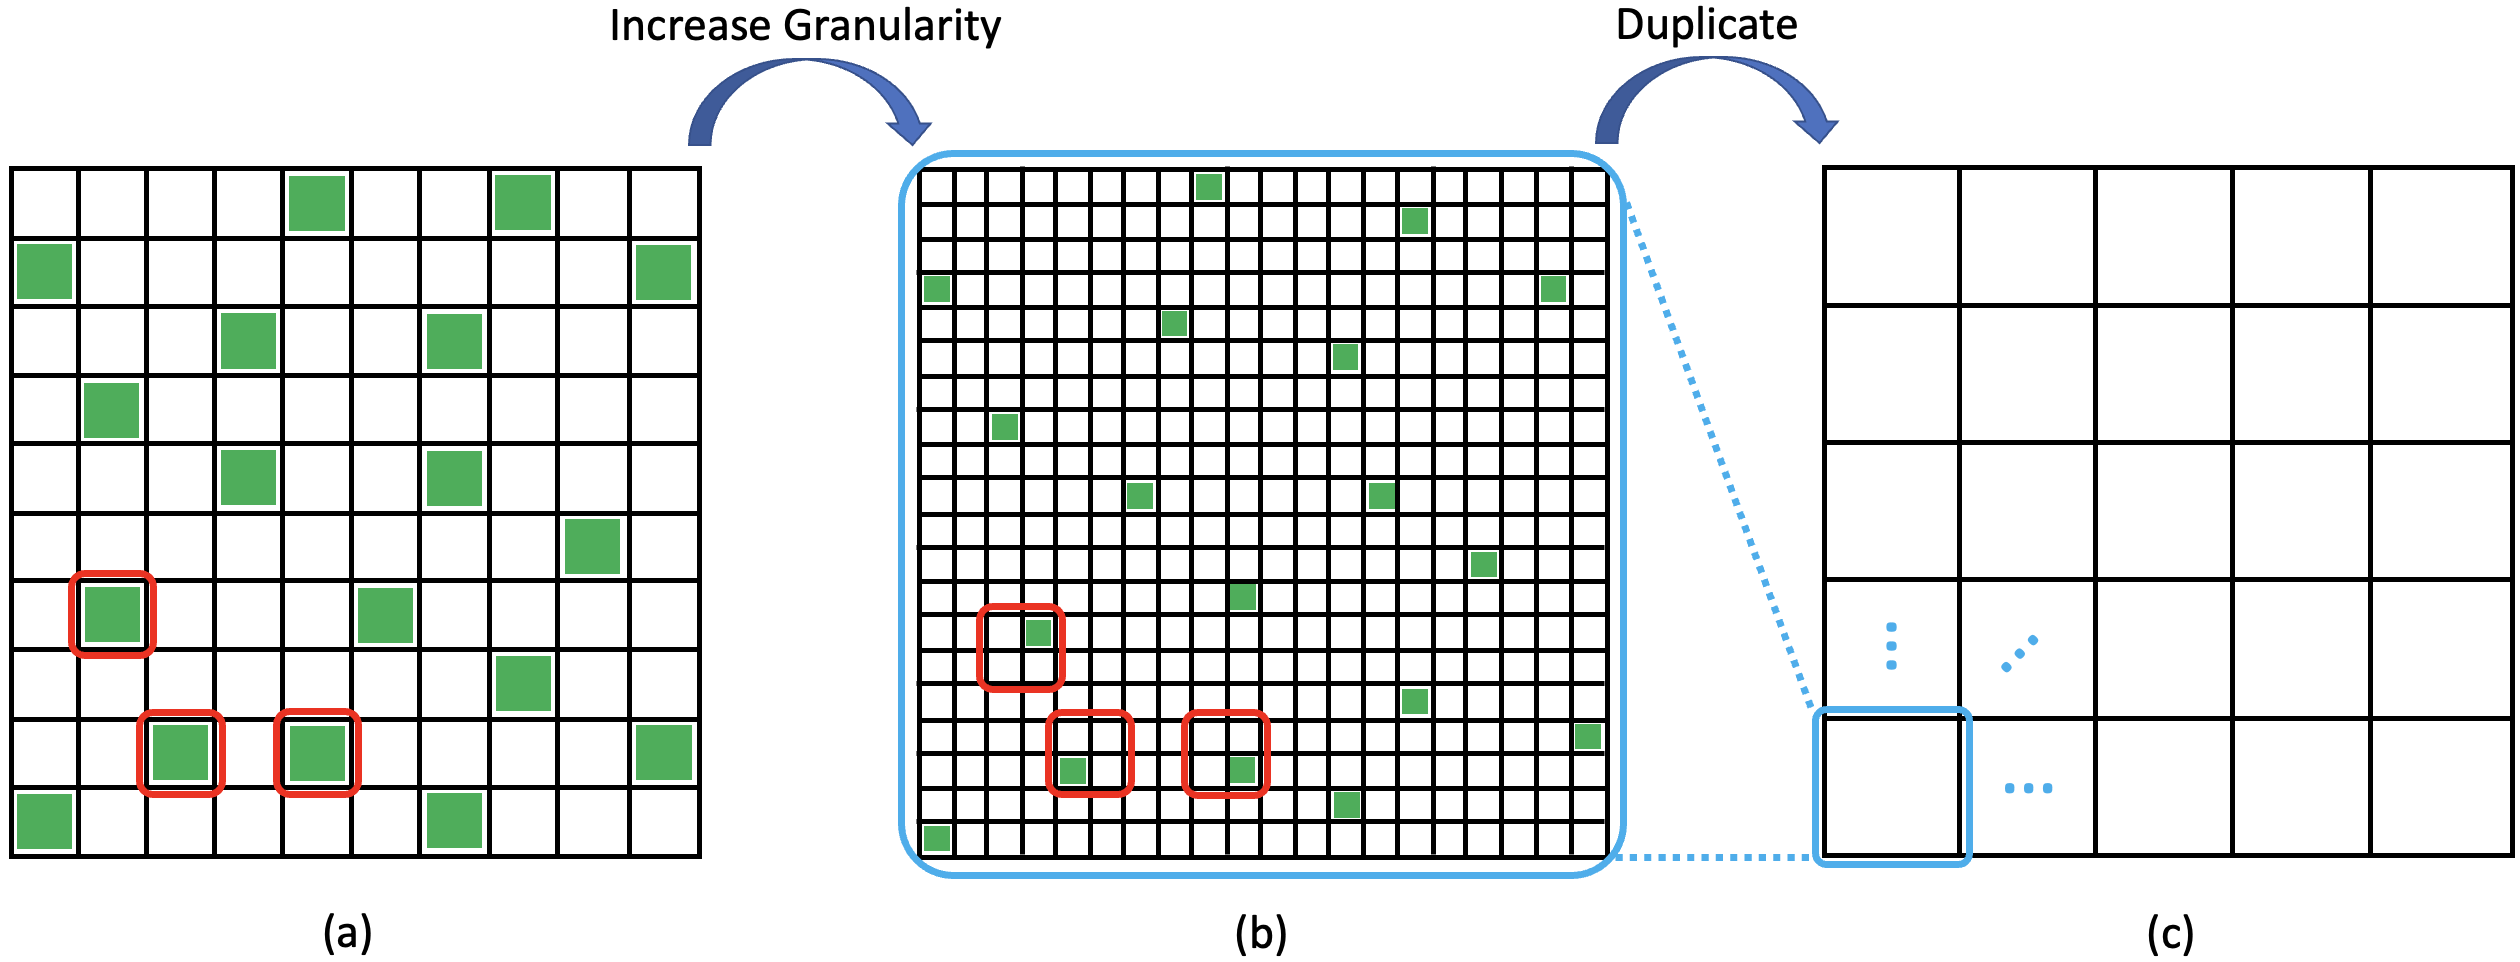
\includegraphics[width=0.98\textwidth]{chapters/wowmom-pmc/figures/testbed.png}
    \caption{(a). The original $10\times10$ testbed grid with 18 sensors (green cells) representing a $32m \times 32m$ area. (b). The $20\times20$ grid (a tile) obtained by replacing each original cell by $2 \times 2$ smaller cells; a sensor, if present in the original cell, is placed in a random cell within the  $2\times2$ grid (see the green cells). (c). The final $100\times100$ grid obtained by duplicating the $20\times20$ tile 25 times using a $5\times5$ pattern. The final geographic area is $160m\times160m$.}
    \label{fig:testbed}
\end{figure}

\begin{figure}
    \centering
    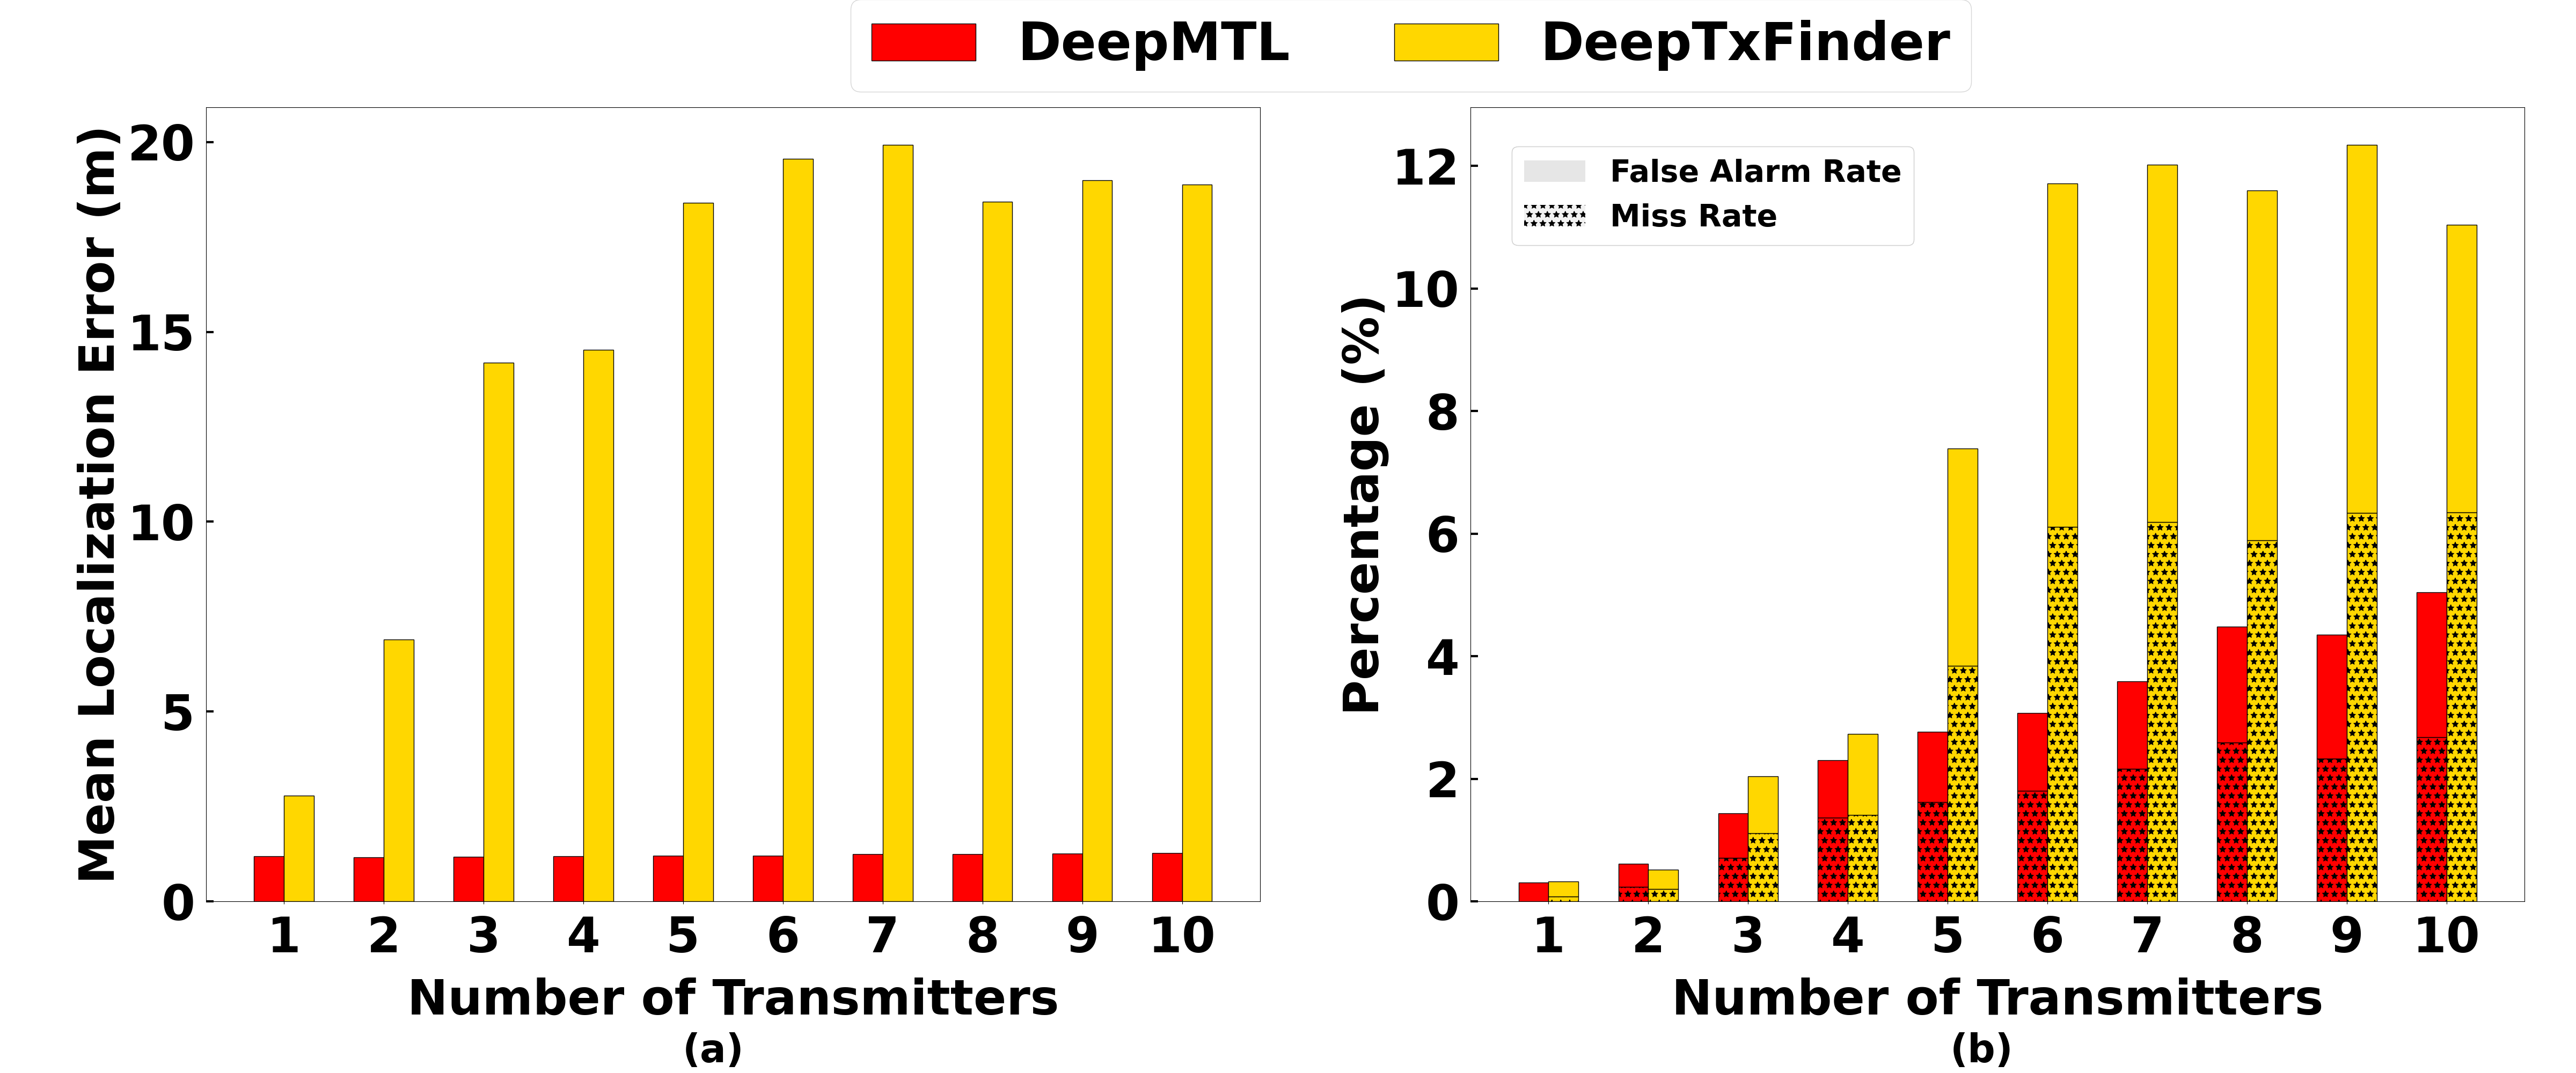
\includegraphics[width=0.95\textwidth]{chapters/wowmom-pmc/figures/ipsn_testbed-error_false_miss_vary_numintru.png}
    \caption{The localization error (a), false alarm rate and miss rate (b) of \our and \deeptx in a real world collected data for varying number of intruders.}
    \label{fig:ipsn}
\end{figure}

\para{Testbed Results.}
The performance of \our on this real world based data is shown in Fig.~\ref{fig:ipsn}.
Compared to \deeptx, \our is significantly better in localization error and false alarm rate and miss rate in almost all cases, which aligns to the results in the previous subsections based on data generated from either log-distance model or SPLAT!.
The localization error of \our in Fig.~\ref{fig:ipsn}(a) is around 1.3 meters.
The error increases mildly with the increase in the number of transmitters.
The localization error in the testbed data is smaller compared to both log-distance data results (Fig.~\ref{fig:logdist-error-vary_numintru}) and SPLAT! data results (Fig.~\ref{fig:splat-error-vary_numintru}).
This is because a grid cell here is representing a smaller area.
In the log-distance data, the localization error is roughly one-fourth the side length of the grid cell. 
In the SPLAT! data result, the localization error is roughly half the side length of its grid length.
In the testbed data, the localization is roughly eighty percent the side length of a grid cell.
So the localization error in the testbed data is the highest relative to the length of a grid cell it represents.
The sum of false alarm rate and miss rate is 3\% when the number of transmitters is five and is 5\% when the number of transmitters is ten.
The results are a little bit worse than the results in the SPLAT! data (Fig.~\ref{fig:splat-missfalse-vary-numintru}), where the sum is 2\% for five transmitters and 4\% for ten transmitters.

